\documentclass{scalatekids-article}
\usepackage[italian]{babel}
\usepackage{tocloft}
\cftsetindents{paragraph}{4em}{5em}
\cftsetindents{subparagraph}{5em}{6em}
\begin{document}
\lfoot{Specifica Tecnica 2.0.0}
\newgeometry{top=3.5cm}
\begin{titlepage}
  \begin{center}
    \begin{center}
      
\includegraphics[width=10cm]{sklogo.png}
    \end{center}
    \vspace{1cm}
    \begin{Huge}
      \begin{center}
        \textbf{Specifica Tecnica}
      \end{center}
    \end{Huge}
    \vspace{11pt}
    \bgroup
    \def\arraystretch{1.0}
    \begin{tabular}{r|l}
      \multicolumn{2}{c}{\textbf{Informazioni sul documento}} \\
      \hline
      \setbox0=\hbox{0.0.1\unskip}\ifdim\wd0=0pt
      \\
      \else
      \textbf{Versione} & 2.0.0\\
      \fi
      \textbf{Redazione} & \multiLineCell[t]{Alberto De Agostini\\Andrea Giacomo Baldan\\Davide Trevisan\\Francesco Agostini\\Giacomo Vanin\\Marco Boseggia}\\
      \textbf{Verifica} & \multiLineCell[t]{Alberto De Agostini\\Andrea Giacomo Baldan\\Davide Trevisan\\Michael Munaro}\\
      \textbf{Approvazione} & \multiLineCell[t]{Marco Boseggia}\\
      \textbf{Uso} & Esterno\\
      \textbf{Lista di Distribuzione} & \multiLineCell[t]{ScalateKids\\Prof. Tullio Vardanega\\Prof. Riccardo Cardin}\\
    \end{tabular}
    \egroup
    \vspace{22pt}
  \end{center}
\end{titlepage}
\restoregeometry
\clearpage
\pagenumbering{Roman}
\setcounter{page}{1}
\begin{flushleft}
  \vspace{0cm}
  {\large\bfseries Diario delle modifiche \par}
\end{flushleft}
\vspace{0cm}
\begin{center}
  \begin{longtable}{| l | l | l | l | p{5cm} |}
    \hline
    Versione & Autore & Ruolo & Data & Descrizione \\
    \hline
    1.4.0 & & & 2016-05-03 & Verifica sezione 4.25 e relative sotto-sezioni\\
    \hline
    1.3.1 & & & 2016-05-02 & Incremento sezione 4.25 e relative sotto-sezioni\\
    \hline
    1.3.0 & & & 2016-04-30 & Verifica sezione 4.24 e relative sotto-sezioni\\
    \hline
    1.2.1 & & & 2016-04-29 & Incremento sezione 4.24 e relative sotto-sezioni\\
    \hline
    1.2.0 & & & 2016-04-28 & Verifica sezione 4.23 e relative sotto-sezioni\\
    \hline
    1.1.0 & & & 2016-04-28 & Verifica sezione 4.22 e sotto-sezione 4.22.4\\
    \hline
    1.0.2 & & & 2016-04-28 & Incremento sezione 4.23 e relative sotto-sezioni\\
    \hline
    1.0.1 & & & 2016-04-27 & Incremento sezione Driver 4.22 e sotto-sezione 4.22.4\\
    \hline
    1.0.0 & Marco Boseggia & Responsabile & 2016-04-08 & Approvazione documento\\
    \hline
    0.8.0 & Andrea Giacomo Baldan & Verificatore & 2016-04-03 & Verifica appendice\\
    \hline
    0.7.1 & Giacomo Vanin & Progettista & 2016-04-03 & Stesura appendice documento\\
    \hline
    0.7.0 & Alberto De Agostini & Verificatore & 2016-04-02 & Verifica tracciamenti (sezione 9)\\
    \hline
    0.6.1 & Francesco Agostini & Progettista & 2016-04-02 & Stesura sezione 9 comprensivo di tutto il tracciamento\\
    \hline
    0.6.0 & Andrea Giacomo Baldan & Verificatore & 2016-04-01 & Verifica sezioni 7 e 8 \\
    \hline
    0.5.2 & Alberto De Agostini & Progettista & 2016-03-31 & Stesura sezione 8\\
    \hline
    0.5.1 & Alberto De Agostini & Progettista & 2016-03-30 & Stesura sezione 7 e sottosezioni\\
    \hline
    0.5.0 & Andrea Giacomo Baldan & Verificatore & 2016-03-28 & Verifica sezione 6 e sottosezioni\\
    \hline
    0.4.1 & Davide Trevisan & Progettista & 2016-03-27 & Stesura sezione 6 e sottosezioni\\
    \hline
    0.4.0 & Michael Munaro & Verificatore & 2016-03-25 & Verifica sezione 5\\
    \hline
    0.3.1 & Giacomo Vanin & Progettista & 2016-03-24 & Stesura sezione 5\\
    \hline
    0.3.0 & Alberto De Agostini & Verificatore & 2016-03-22 & Verifica sezioni da 4.6 a 4.13\\
    \hline
    0.2.2 & Marco Boseggia & Progettista & 2016-03-22 & Stesura sezioni 4.10 4.11 4.12 4.13\\
    \hline
    0.2.1 & Marco Boseggia & Progettista & 2016-03-21 & Stesura sezioni 4.6 4.7 4.8 4.9\\
    \hline
    0.2.0 & Michael Munaro & Verificatore & 2016-03-21 & Verifica sottosezioni 3.1 3.2 4.1 4.2 4.3 4.4 4.5\\
    \hline
    0.1.2 & Andrea Giacomo Baldan & Progettista & 2016-03-17 & Stesura sottosezioni 4.1 4.2 4.3 4.4 4.5\\
    \hline
    0.1.1 & Andrea Giacomo Baldan & Progettista & 2016-03-17 & Stesura sottosezioni 3.1 3.2\\
    \hline
    0.1.0 & Michael Munaro & Verificatore & 2016-03-16 & Verifica sezioni 1 e 2\\
    \hline
    0.0.2 & Marco Boseggia & Progettista & 2016-02-26 & Stesura sezioni 1 e 2\\
    \hline
    0.0.1 & Andrea Giacomo Baldan & Amministratore & 2016-02-26 & Creazione scheletro del documento\\
    \hline
  \end{longtable}
\end{center}
\newpage
\tableofcontents
\newpage
\pagenumbering{arabic}

\section{Sommario}

\subsection{Scopo del documento}

Il seguente documento ha lo scopo di descrivere la progettazione ad alto livello
che il gruppo \textit{ScalateKids} ha scelto per il
progetto \textbf{Actorbase}.\\  Sarà descritta l'\gloss{architettura} generale
del progetto, in particolare  la scelta dei \gloss{design pattern} e delle
componenti che andranno a comporre il software.

\prodPurpose

\glossExpl

\subsection{Riferimenti}

\subsubsection{Normativi}

\begin{itemize}

\item\textbf{Capitolato d'appalto C1:} \textit{Actorbase: a NoSQL DB based on the Actor model;}\\
  \url{http://www.math.unipd.it/~tullio/IS-1/2015/Progetto/C1.pdf}
\item\textbf{Norme di Progetto:}
  \href{run:../Interni/NormeDiProgetto\_v3.0.0.pdf}{Norme di Progetto v3.0.0.}
\end{itemize}

\subsubsection{Informativi}

\begin{itemize}
\item\textbf{Piano di Progetto:} \href{run:./PianoDiProgetto\_v3.0.0.pdf}{Piano di Progetto v3.0.0}
\item\textbf{Dispense fornite dall'insegnamento Ingegneria del Software mod.A:}\\
  \url{http://www.math.unipd.it/~tullio/IS-1/2015/}
\item\textbf{Documentazione di \gloss{Akka} su \gloss{Scala}:}
  \url{http://doc.akka.io/docs/akka/2.4.2/scala.html}
\item\textbf{SBT\ -\ Scala build tool:}
  \url{http://www.scala-sbt.org/index.html}
\item\textbf{Scala Pickling\ -\ Fast, Customizable, Boilerplate-Free Serialization for Scala:} Libreria di serializzazione e deserializzazione
  multiformato, pieno supporto \gloss{JSON} (JavaScript Object Notation) e
  serializzazione in binario \url{http://lampwww.epfl.ch/~hmiller/pickling}
\item\textbf{Spray\ -\ an open-source toolkit for building REST/HTTP-based integration layers on top of Scala and Akka}:
  Libreria per la gestione di richieste \gloss{HTTP}(HyperText Transfert Protocol) in modo asincrono, basata sul modello ad
  attori offerto dalla libreria Akka. \url{http://spray.io/}
\item\textbf{REST\ -\ Representational State Transfer:} Architettura software
  per sistemmi di \gloss{ipertesto} distribuiti, rappresenta un sistema di
  localizzazione e richiesta risorse \gloss{stateless}, poggia su \gloss{HTTP}
  come protocollo di comunicazione \url{https://en.wikipedia.org/wiki/Representational_state_transfer}
\end{itemize}

\newpage

\section{Tecnologie utilizzate}

In questa sezione saranno descritte le tecnologie scelte per lo sviluppo del
progetto \textbf{Actorbase} e le motivazioni che ci hanno spinto a sceglierle.

\subsection{Akka}

La scelta della libreria \gloss{Akka} è stata dettata dal capitolato, tuttavia
l'avremmo scelta comunque per i seguenti motivi:
\begin{itemize}
\item\textbf{Implementazione del \gloss{modello ad attori}:} \gloss{Akka}
  rende semplice la creazione e l'utilizzo degli \gloss{attori}. Grazie a ciò è
  possibile creare facilmente architetture ad eventi estremamente concorrenti e
  viene naturale la distribuibilità del progetto e l'asincronia tra i processi;
\item\textbf{Tolleranza agli errori:} \gloss{Akka} implementa un sistema di
  gerarchia di supervisori. Questa gerarchia consente ai supervisori di un
  \gloss{attore}, nel caso in cui quest'ultimo lanci un'eccezione, di mandarlo
  in \gloss{crash} e farlo poi ripartire. In questo modo il sistema è resiliente
  agli errori;
\item\textbf{Persistenza:} Ogni messaggio ricevuto da ciascun \gloss{attore}
  può essere salvato in maniera tale che al riavvio esso possa riprendere dallo
  stato precedente al suo spegnimento.
\end{itemize}

\subsection{Scala}

Il capitolato richiede l'utilizzo di un linguaggio di programmazione a scelta
tra \gloss{Scala} e \gloss{Java}. Abbiamo scelto \gloss{Scala} per i seguenti
motivi:

\begin{itemize}
\item\textbf{\gloss{Programmazione funzionale}:} Questa tecnica di
  programmazione evita che ci siano degli effetti collaterali tra funzioni,
  rendendole quindi \gloss{thread-safe};
\item\textbf{Implementazione di Akka:} \gloss{Akka} risulta più
  facilmente implementabile in \gloss{Scala} che in \gloss{Java}. Questo perché
  la \gloss{programmazione funzionale} con i suoi paradigmi si integra meglio
  con il \gloss{modello ad attori};
\item\textbf{Implementazione di DSL:} Scala si presta alla creazione di \gloss{DSL}
  in maniera nativa, sia di tipo esterno che di tipo interno, senza necessariamente
  utilizzare librerie esterne o appoggiarsi a framework appositi;
\item\textbf{Integrazione con librerie Java:} In Scala è possibile usufruire di molte
  librerie sviluppate in ambiente Java in quanto utilizza lo stesso modello di compilazione
  generando dei \gloss{file} in \gloss{bytecode}.
\end{itemize}

Tuttavia presenta alcuni svantaggi:

\begin{itemize}
\item\textbf{Curva di apprendimento:} Scala introduce paradigmi di programmazione funzionale
  applicati al paradigma ad oggetti, inoltre ha una sintassi molto espressiva e questo può
  rallentare significativamente il processo di apprendimento per i neofiti;
\item\textbf{Librerie Java:} La possibilità di usufruire di molte librerie Java, pur essendo
  considerato positivo, ha anche il lato negativo di doversi appoggiare a documentazioni specifiche
  per linguaggio Java, e questo può portare a difficili comprensioni del comportamento della libreria
  in Scala, specie nel caso in cui la compatibilità non sia al 100\%.
\end{itemize}

\subsection{sbt}

Sbt (Simple Build Tool) è un ambiente di \gloss{build} simile alla controparte Java \gloss{Maven} o
\gloss{Ant}. Fornito di \gloss{console} e strumenti di compilazione ed
esecuzione per progetti Scala, è stato scelto per i seguenti vantaggi:
\begin{itemize}
\item Semplice configurazione mediante file;
\item \gloss{REPL} Scala integrata;
\item Facilmente integrabile all'interno di \gloss{IDE} e editor;
\item Gestione semplificata delle dipendenze;
\item Gestione semplificata del processo di \gloss{build}.
\end{itemize}

\section{Descrizione architettura}

\subsection{Metodo e formalismo di specifica}

L'esposizione dell'architettura segue la metodologia \gloss{top-down},
descrivendo l'architettura iniziando dalle componenti generali e scendendo
nel dettaglio. Seguirà quindi la descrizione dei \gloss{package} seguiti dalla descrizione
in dettaglio delle classi e interfacce che vi appartengono, specificando
per ognuna la funzione e le relazioni in ingresso ed uscita. Il formalismo
cromatico utilizzato sarà conforme a quanto specificato in \textit{Norme Di Progetto}.\\
Successivamente si illustreranno i \gloss{Design Pattern} e la loro applicazione
all'interno delle componenti, con un approfondimento del loro funzionamento
in \hyperref[sec:appendice]{appendice A}.\\
Nel trattare le componenti, si chiarisce che sono da intendersi come \gloss{package}
e i due termini verranno quindi usati come sinonimi.\\

\subsection{Architettura generale}

Macroscopicamente il sistema si suddivide in due componenti principali,
assimilabili ad un paradigma \gloss{Client}-\gloss{Server}, il sistema ad attori dove risiedono
la struttura della base di dati ed un \gloss{server} TCP (Transmission Control Protocol)
pronto a ricevere comandi dall'esterno rappresentano la componente \gloss{server}, la
Command Line Interface (\gloss{CLI}) rappresenta la componente \gloss{client} mediante la quale
è possibile inviare comandi al sistema e ricevere l'output prodotto da essi.
Essa farà uso della componente \gloss{driver} per comunicare con il sistema lato
\gloss{server} mediante il protocollo di comunicazione testuale \hyperref[sec:RESP]{RESP}.\\

\begin{figure}[H]
  \begin{center}
    \includegraphics[width=0.2\textwidth,keepaspectratio]{RP/RP-ClientServer.png}
    \caption{Diagramma architettura concettuale}
  \end{center}
\end{figure}

\subsection{Protocollo di comunicazione Client-Server}
\label{sec:HTTP}

\textbf{Actorbase} è stato concepito come sistema \gloss{RESTful} con
possibilità di utilizzo come \gloss{web-service}. La connessione è quindi di
tipo Stateless, in quanto ogni richiesta non ha nulla a che fare con lo storico
di richieste precedenti.

\section{Componenti}

L'architettura principale del progetto è stata suddivisa in tre macro-componenti, rispettivamente
\textbf{cli}, \textbf{driver} e \textbf{actorsystem}; contenute all'interno del package
generale \textbf{actorbase}.

\subsection{actorbase}
\label{sec:actorbase}

\begin{figure}[H]
  \begin{center}
    \includegraphics[width=0.9\textwidth,keepaspectratio]{RQ/Architettura-AltoLivello.png}
    \caption{Diagramma componenti principali}
  \end{center}
\end{figure}

\subsubsection{Descrizione}

La componente principale rappresentata dal package globale \textbf{actorbase}.

\subsubsection{Package contenuti}

\begin{itemize}
\item \hyperref[sec:actorbase::cli]{actorbase::cli};
\item \hyperref[sec:actorbase::driver]{actorbase::driver};
\item \hyperref[sec:actorbase::actorsystem]{actorbase::actorsystem}.
\end{itemize}

Rappresentano le tre macro-componenti del sistema.

%%%%%%%%%%%%%%%%%%%%%%%%%%%%%%%%%%%%%%%%%%%%%%%%%%%%%%%%%%%%%%%%%%%%
% ACTORSYSTEM PARTE                           %
%%%%%%%%%%%%%%%%%%%%%%%%%%%%%%%%%%%%%%%%%%%%%%%%%%%%%%%%%%%%%%%%%%%%

\subsection{actorbase::actorsystem} %TODO da fare actorsystem
\label{sec:actorbase::actorsystem}

\begin{figure}[H]
  \begin{center}
    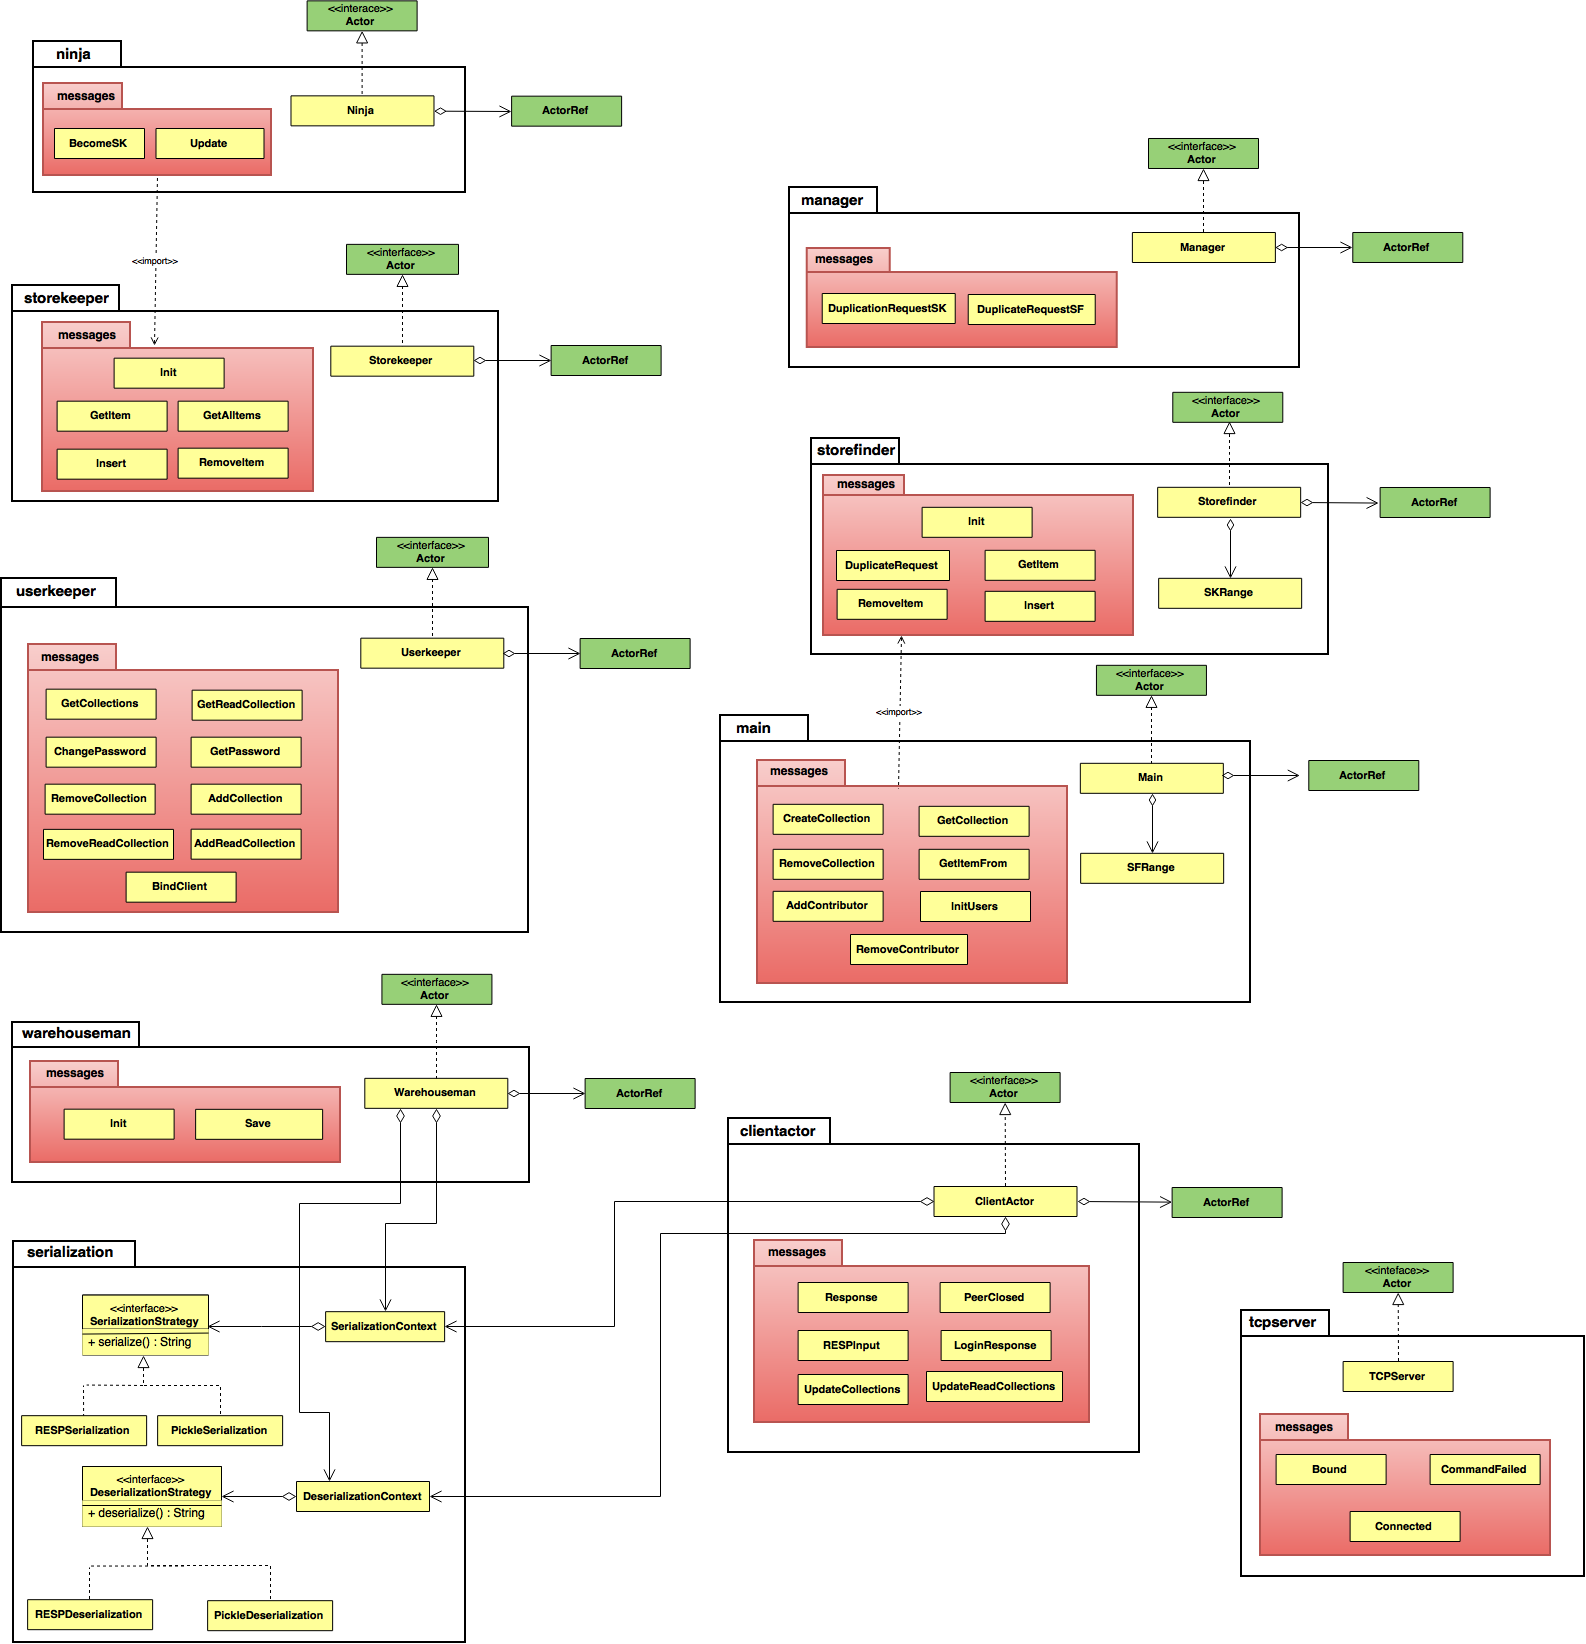
\includegraphics[width=0.9\textwidth,keepaspectratio]{RQ/Actorsystem.png}
    \caption{Actorsystem, visione generale}
  \end{center}
\end{figure}

\subsubsection{Descrizione}

\gloss{Package} che raggruppa tutte le componenti del sistema che
rappresentano il \gloss{server}.

\subsubsection{Package contenuti}

\begin{itemize}
\item \hyperref[sec:actorbase::actorsystem::clientactor]{actorbase::actorsystem::clientactor};
\item \hyperref[sec:actorbase::actorsystem::httpserver]{actorbase::actorsystem::httpserver};
\item \hyperref[sec:actorbase::actorsystem::storefinder]{actorbase::actorsystem::storefinder};
\item \hyperref[sec:actorbase::actorsystem::storekeeper]{actorbase::actorsystem::storekeeper};
\item \hyperref[sec:actorbase::actorsystem::userfinder]{actorbase::actorsystem::userfinder};
\item \hyperref[sec:actorbase::actorsystem::userkeeper]{actorbase::actorsystem::userkeeper};
\item \hyperref[sec:actorbase::actorsystem::warehouseman]{actorbase::actorsystem::warehouseman};
\item \hyperref[sec:actorbase::actorsystem::manager]{actorbase::actorsystem::manager};
\item \hyperref[sec:actorbase::actorsystem::main]{actorbase::actorsystem::main};
\item \hyperref[sec:actorbase::actorsystem::serialization]{actorbase::actorsystem::utils}.
\end{itemize}

\subsubsection{Interazioni con altre componenti}

\begin{itemize}
\item \hyperref[sec:actorbase::driver]{actorbase::driver};
\item Akka.
\end{itemize}


\subsection{actorbase::actorsystem::utils}
\label{sec:actorbase::actorsystem::utils}

\begin{figure}[H] %TODO aggiungere immagine
  \begin{center}
    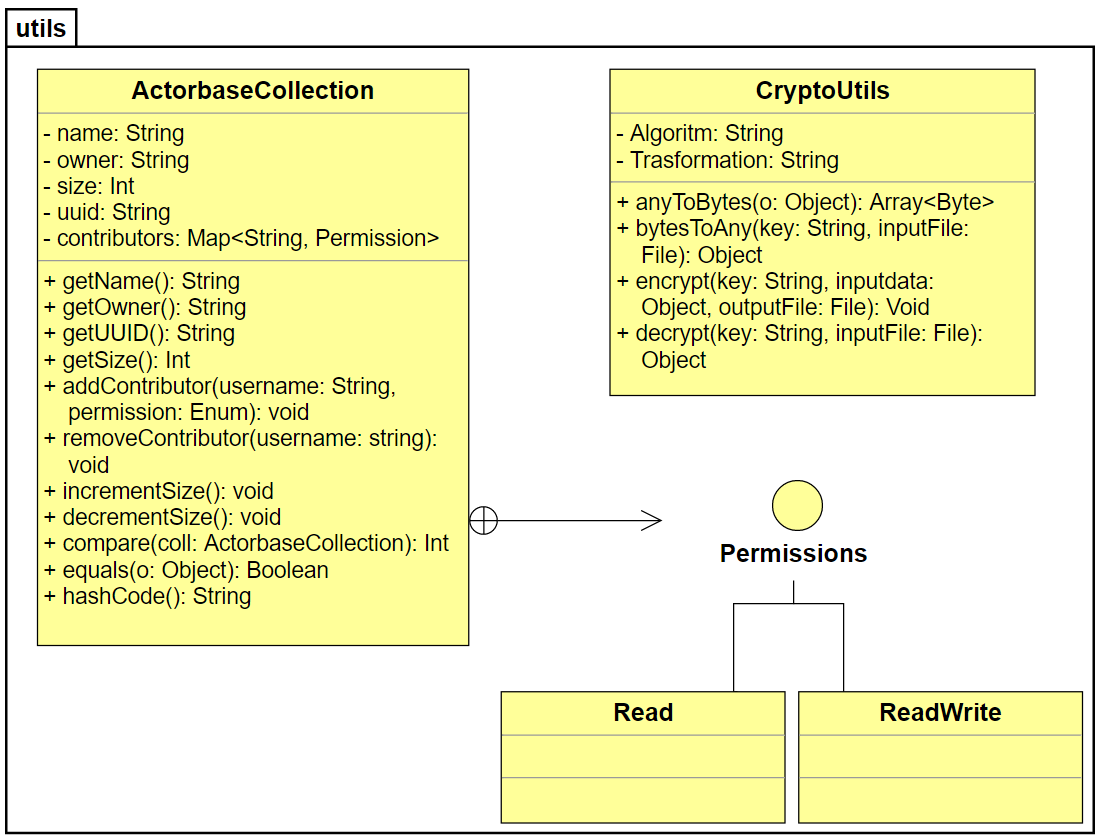
\includegraphics[width=1.0\textwidth,keepaspectratio]{RQ/utils.png}
    \caption{Package actorsystem::utils}
  \end{center}
\end{figure}

\subsubsection{Descrizione}
\gloss{Package} contenente diverse classi di utilità.

\subsubsection{Interazioni con altre componenti}

\begin{itemize}
\item \hyperref[sec:actorbase::actorsystem::storekeeper]{actorbase::actorsystem::storekeeper};
\item \hyperref[sec:actorbase::actorsystem::storefinder]{actorbase::actorsystem::storefinder};
\item \hyperref[sec:actorbase::actorsystem::userkeeper]{actorbase::actorsystem::userkeeper};
\item \hyperref[sec:actorbase::actorsystem::warehouseman]{actorbase::actorsystem::warehouseman};
\item \hyperref[sec:actorbase::actorsystem::main]{actorbase::actorsystem::main};
\item \hyperref[sec:actorbase::actorsystem::clientactor]{actorbase::actorsystem::clientactor}.
\end{itemize}

\subsubsection{Classi}

%%%%%%%%%%%%%%%%%%%%%%%%%%%%%%%%%%%%%%%%%%%%%%%%%%%%%%%%%%%%%%%%%%%%%%%%%
%%%%%%%%%%%%%%%%%%%%%%%%%%%%%%%%%%%%%%%%%%%%%%%%%%%%%%%%%%%%%%%%%%%%%%%%%

\paragraph{KeyRange}
\label{sec:actorbase::actorsystem::utils::KeyRange}

\subparagraph{Descrizione}
Classe atta a modellare un intervallo di chiavi.\\Viene utilizzata da diversi
attori.

\subparagraph{Utilizzo}
Viene utilizzata da diversi attori del sistema. Questa classe espone metodi
getter, un metodo compare e un metodo per controllare se una determinata
stringa fa parte di questo intervallo di chiavi.

\subparagraph{Realizza}
\begin{itemize}
\item trait scala.math.Ordered.orderingToOrdered
\end{itemize}

\subparagraph{Interazioni con altre classi}

\begin{itemize}
\item \hyperref[sec:actorbase::actorsystem::storekeeper::Storekeeper]{actorbase::actorsystem::storekeeper::Storekeeper};
\item \hyperref[sec:actorbase::actorsystem::storefinder::Storefinder]{actorbase::actorsystem::storefinder::Storefinder};
\item \hyperref[sec:actorbase::actorsystem::main::Main]{actorbase::actorsystem::main::Main}.
\end{itemize}

%%%%%%%%%%%%%%%%%%%%%%%%%%%%%%%%%%%%%%%%%%%%%%%%%%%%%%%%%%%%%%%%%%%%%%%%%
%%%%%%%%%%%%%%%%%%%%%%%%%%%%%%%%%%%%%%%%%%%%%%%%%%%%%%%%%%%%%%%%%%%%%%%%%

\paragraph{CollectionRange}
\label{sec:actorbase::actorsystem::utils::CollectionRange}

\subparagraph{Descrizione}
Classe atta a modellare un intervallo di chiavi di una specifica collezione.

\subparagraph{Utilizzo}
Viene utilizzata da diversi attori del sistema. Questa classe espone metodi
getter, un metodo per il confronto della collezione, un meotodo per il
confronto del range delle chiavi e un metodo compare.

\subparagraph{Realizza}
\begin{itemize}
\item trait scala.math.Ordered.orderingToOrdered
\end{itemize}

\subparagraph{Interazioni con altre classi}

\begin{itemize}
\item \hyperref[sec:actorbase::actorsystem::storefinder::Storefinder]{actorbase::actorsystem::storefinder::Storefinder};
\item \hyperref[sec:actorbase::actorsystem::main::Main]{actorbase::actorsystem::main::Main}.
\end{itemize}

%%%%%%%%%%%%%%%%%%%%%%%%%%%%%%%%%%%%%%%%%%%%%%%%%%%%%%%%%%%%%%%%%%%%%%%%%
%%%%%%%%%%%%%%%%%%%%%%%%%%%%%%%%%%%%%%%%%%%%%%%%%%%%%%%%%%%%%%%%%%%%%%%%%

\paragraph{CryptoUtils}
\label{sec:actorbase::actorsystem::utils::CryptoUtils}

\subparagraph{Descrizione}
Classe atta a criptare e decriptare i dati per il salvataggio e la lettura dei dati su disco.

\subparagraph{Utilizzo}
Viene utilizzata dall'attore di tipo \gloss{Warehouseman} per il salvataggio e la lettura del database su disco.

\subparagraph{Interazioni con altre classi}

\begin{itemize}
\item \hyperref[sec:actorbase::actorsystem::warehouseman::Warehouseman]{actorbase::actorsystem::warehouseman::Warehouseman}.
\end{itemize}

%%%%%%%%%%%%%%%%%%%%%%%%%%%%%%%%%%%%%%%%%%%%%%%%%%%%%%%%%%%%%%%%%%%%%%%%%%%%%%
%%%%%%%%%%%%%%%%%%%%%%%%%%%%%%%%%%%%%%%%%%%%%%%%%%%%%%%%%%%%%%%%%%%%%%%%%%%%%%

\paragraph{ActorbaseCollection}
\label{sec:actorbase::actorsystem::utils::ActorbaseCollection}

\subparagraph{Descrizione}
Classe atta a modellare una collezione del sistema actorbase.

\subparagraph{Utilizzo}
Viene utilizzata da diversi attori del sistema. Questa classe espone metodi
getter e un meotodo per il confronto con un altro oggetto ActorbaseCollection.

\subparagraph{Realizza}
\begin{itemize}
\item trait scala.math.Ordered
\end{itemize}

\subparagraph{Interazioni con altre classi}

\begin{itemize}
\item \hyperref[sec:actorbase::actorsystem::storekeeper::Storekeeper]{actorbase::actorsystem::storekeeper::Storekeeper};
\item \hyperref[sec:actorbase::actorsystem::storefinder::Storefinder]{actorbase::actorsystem::storefinder::Storefinder};
\item \hyperref[sec:actorbase::actorsystem::userkeeper::Userkeeper]{actorbase::actorsystem::userkeeper::Userkeeper};
\item \hyperref[sec:actorbase::actorsystem::main::Main]{actorbase::actorsystem::main::Main};
\item \hyperref[sec:actorbase::actorsystem::clientactor::ClientActor]{actorbase::actorsystem::clientactor::ClientActor}.
\end{itemize}

%%%%%%%%%%%%%%%%%%%%%%%%%%%%%%%%%%%%%%%%%%%%%%%%%%%%%%%%%%%%%%%%%%%%%%%%%
%%%%%%%%%%%%%%%%%%%%%%%%%%%%%%%%%%%%%%%%%%%%%%%%%%%%%%%%%%%%%%%%%%%%%%%%%
%%%%%%%%%%%%%%%%%%%%%%%%%%%%%%%%%%%%%%%%%%%%%%%%%%%%%%%%%%%%%%%%%%%%%%%%%

\subsection{actorbase::actorsystem::clientactor}
\label{sec:actorbase::actorsystem::clientactor}

\begin{figure}[H]
  \begin{center}
    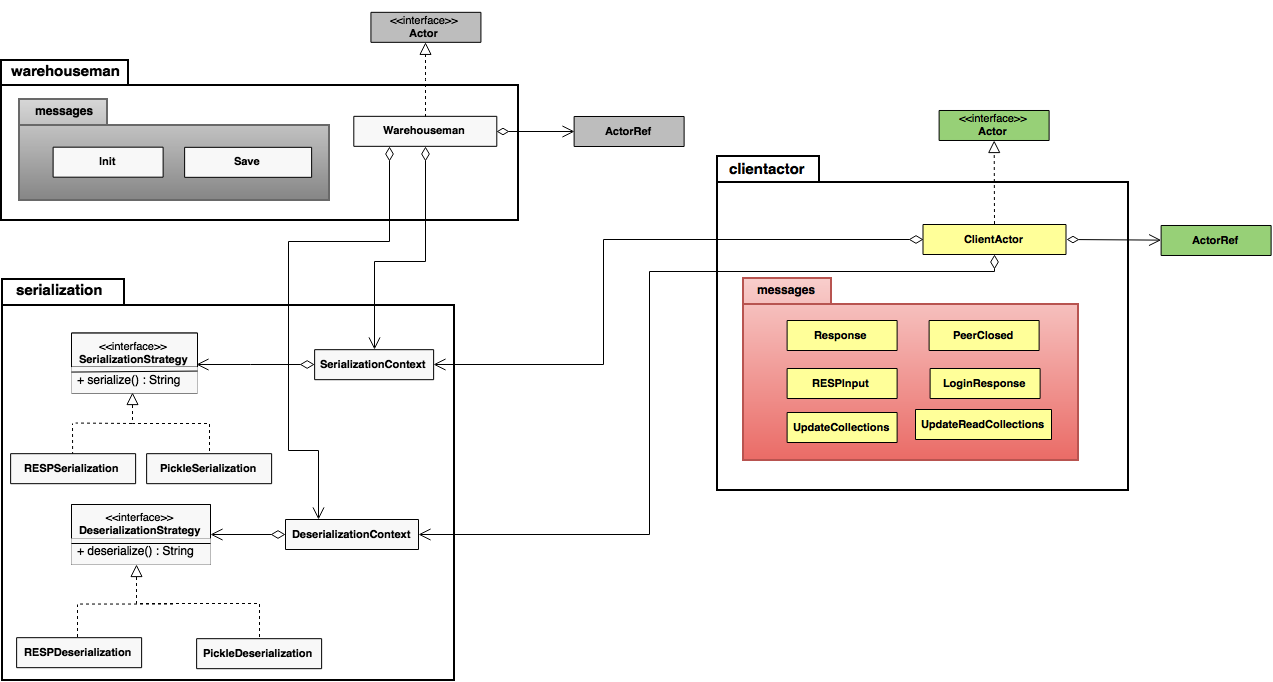
\includegraphics[width=1.0\textwidth,keepaspectratio]{RQ/Clientactor.png}
    \caption{ACtorsystem: package Clientactor}
  \end{center}
\end{figure}

\subsubsection{Descrizione}

\gloss{Package} per l'\gloss{attore} con cui si interfaccerà il \gloss{driver}.

\subsubsection{Package contenuti}

\begin{itemize}
\item \hyperref[sec:actorbase::actorsystem::clientactor::messages]{actorbase::actorsystem::clientactor::messages}.
\end{itemize}

\subsubsection{Interazioni con altre componenti}

\begin{itemize}
\item \hyperref[sec:actorbase::actorsystem::httpserver]{actorbase::actorsystem::\allowbreak{}httpserver};
\item \hyperref[sec:actorbase::driver::client::ActorbaseClient]{actorbase::driver::\allowbreak{}client::\allowbreak{}ActorbaseClient};
\item spray.json;
\item spray.routing;
\item akka.actor;
\item com.github.t3hnar.bcrypt.
\end{itemize}

\subsubsection{Classi}

\paragraph{actorbase::actorsystem::clientactor::Authenticator}
\label{sec:actorbase::actorsystem::clientactor::Authenticator}

\subparagraph{Descrizione}

Classe astratta usata per effettuare la validazione di un login.

\subparagraph{Utilizzo}

Questa classe viene usata dalla classe che la realizza per effettuare il controllo
delle credenziali di login.

\paragraph{actorbase::actorsystem::clientactor::CollectionApi}
\label{sec:actorbase::actorsystem::clientactor::CollectionApi}

\subparagraph{Descrizione}

Classe astratta usata per analizzare le route che richiedono operazioni su collezioni.

\subparagraph{Utilizzo}

Questa classe viene usata dalla classe che la realizza per effettuare l'analisi
delle route che richiedono operazioni su collezioni.

\subparagraph{Interazioni con altre classi}

\begin{itemize}
\item \item \hyperref[sec:actorbase::actorsystem::utils::ActorbaseCollection]{actorbase::actorsystem::utils::ActorbaseCollection};
\item spray.routing.
\end{itemize}

\paragraph{actorbase::actorsystem::clientactor::ItemApi}
\label{sec:actorbase::actorsystem::clientactor::ItemApi}

\subparagraph{Descrizione}

Classe astratta usata per analizzare le route che richiedono operazioni su item.

\subparagraph{Utilizzo}

Questa classe viene usata dalla classe che la realizza per effettuare l'analisi
delle route che richiedono operazioni su item.

\subparagraph{Interazioni con altre classi}

\begin{itemize}
\item spray.routing.
\end{itemize}

\paragraph{actorbase::actorsystem::clientactor::UserApi}
\label{sec:actorbase::actorsystem::clientactor::UserApi}

\subparagraph{Descrizione}

Classe astratta usata per analizzare le route che richiedono operazioni su utenti.

\subparagraph{Utilizzo}

Questa classe viene usata dalla classe che la realizza per effettuare l'analisi
delle route che richiedono operazioni su utenti.

\subparagraph{Interazioni con altre classi}

\begin{itemize}
\item spray.routing.
\end{itemize}

\paragraph{actorbase::actorsystem::clientactor::ClientActor} %TODO da fare
\label{sec:actorbase::actorsystem::clientactor::ClientActor}

\subparagraph{Descrizione}

Classe che rappresenta l'\gloss{attore} con cui si interfaccia il \gloss{driver} dopo
la connessione.

\subparagraph{Utilizzo}

Questo \gloss{attore} riceve le richieste da \hyperref[sec:actorbase::driver::client::Connection]{actorbase::driver::client::Connection}
e si occupa di inviare messaggi al \hyperref[sec:actorbase::actorsystem::main::Main]{Main}. \\
Questa classe inoltre si occupa di capire che tipo di richiesta è stata fatta dal \gloss{driver} basandosi sulla route di quest'ultima.

\subparagraph{Classi ereditate}

\begin{itemize}

\item akka::actor::Actor;
\item \hyperref[com::actorbase::actorsystem::clientactor::Authenticator]{com::actorbase::actorsystem::clientactor::Authenticator};
\item \hyperref[com::actorbase::actorsystem::clientactor::CollectionApi]{com::actorbase::actorsystem::clientactor::CollectionApi};
\item \hyperref[com::actorbase::actorsystem::clientactor::RestApi]{com::actorbase::actorsystem::clientactor::RestApi};.

\end{itemize}

\subparagraph{Interazioni con altre classi}

\begin{itemize}
\item \hyperref[sec:actorbase::actorsystem::httpserver::HTTPServer]{actorbase::actorsystem::\allowbreak{}httpserver::\allowbreak{}HTTPServer};
\item \hyperref[sec:actorbase::driver::client::ActorbaseClient]{actorbase::driver::\allowbreak{}client::\allowbreak{}ActorbaseClient}.
\end{itemize}

\subsection{actorbase::actorsystem::clientactor::messages}
\label{sec:actorbase::actorsystem::clientactor::messages}

\begin{figure}[H]
  \begin{center}
    \includegraphics[width=0.6\textwidth,keepaspectratio]{RQ/classiDiag/messages-client.png}
    \caption{Actorsystem: package messages del clientactor}
  \end{center}
\end{figure}

\subsubsection{Descrizione}

\gloss{Package} che contiene tutti i messaggi che possono essere ricevuti dal
\hyperref[sec:actorbase::actorsystem::clientactor::ClientActor]{ClientActor}.

\subsubsection{Classi}

\paragraph{actorbase::actorsystem::clientactor::messages::Response}
\label{sec:actorbase::actorsystem::clientactor::messages::Response}

\subparagraph{Descrizione}

Messaggio che rappresenta la risposta da parte del \gloss{server} da inoltrare
al \gloss{driver}.

\subparagraph{Utilizzo}

Quando \hyperref[sec:actorbase::actorsystem::clientactor::ClientActor]{actorbase::actorsystem::clientactor::ClientActor}
riceve questo messaggio il contenuto di quest'ultimo viene
mandato a \hyperref[sec:actorbase::driver::client::ActorbaseClient]{actorbase::driver::\allowbreak{}client::\allowbreak{}ActorbaseClient}.

\subparagraph{Interazioni con altre classi}

\begin{itemize}
\item spray.json.
\end{itemize}

\paragraph{actorbase::actorsystem::clientactor::messages::MapResponse}
\label{sec:actorbase::actorsystem::clientactor::messages::MapResponse}

\subparagraph{Descrizione}

Messaggio che rappresenta la risposta da parte del \gloss{server} ad una ricerca da inoltrare
al \gloss{driver}.

\subparagraph{Utilizzo}

Quando \hyperref[sec:actorbase::actorsystem::clientactor::ClientActor]{ClientActor}
riceve questo messaggio il contenuto di quest'ultimo viene
mandato a \hyperref[sec:actorbase::driver::client::ActorbaseClient]{actorbase::driver::\allowbreak{}client::\allowbreak{}ActorbaseClient}.

\subparagraph{Interazioni con altre classi}

\begin{itemize}
\item spray.json.
\end{itemize}

%%%%%%%%%%%%%%%%%%%%%%%%%%%%%%%%%%%%%%%%%%%%%%%%%%%%%%%%%%%%%%%%%%%%%%%%%
%%%%%%%%%%%%%%%%%%%%%%%%%%%%%%%%%%%%%%%%%%%%%%%%%%%%%%%%%%%%%%%%%%%%%%%%%
%%%%%%%%%%%%%%%%%%%%%%%%%%%%%%%%%%%%%%%%%%%%%%%%%%%%%%%%%%%%%%%%%%%%%%%%%

\subsection{actorbase::actorsystem::httpserver} %TODO da ricontrollare
\label{sec:actorbase::actorsystem::httpserver}

\begin{figure}[H]
  \begin{center}
    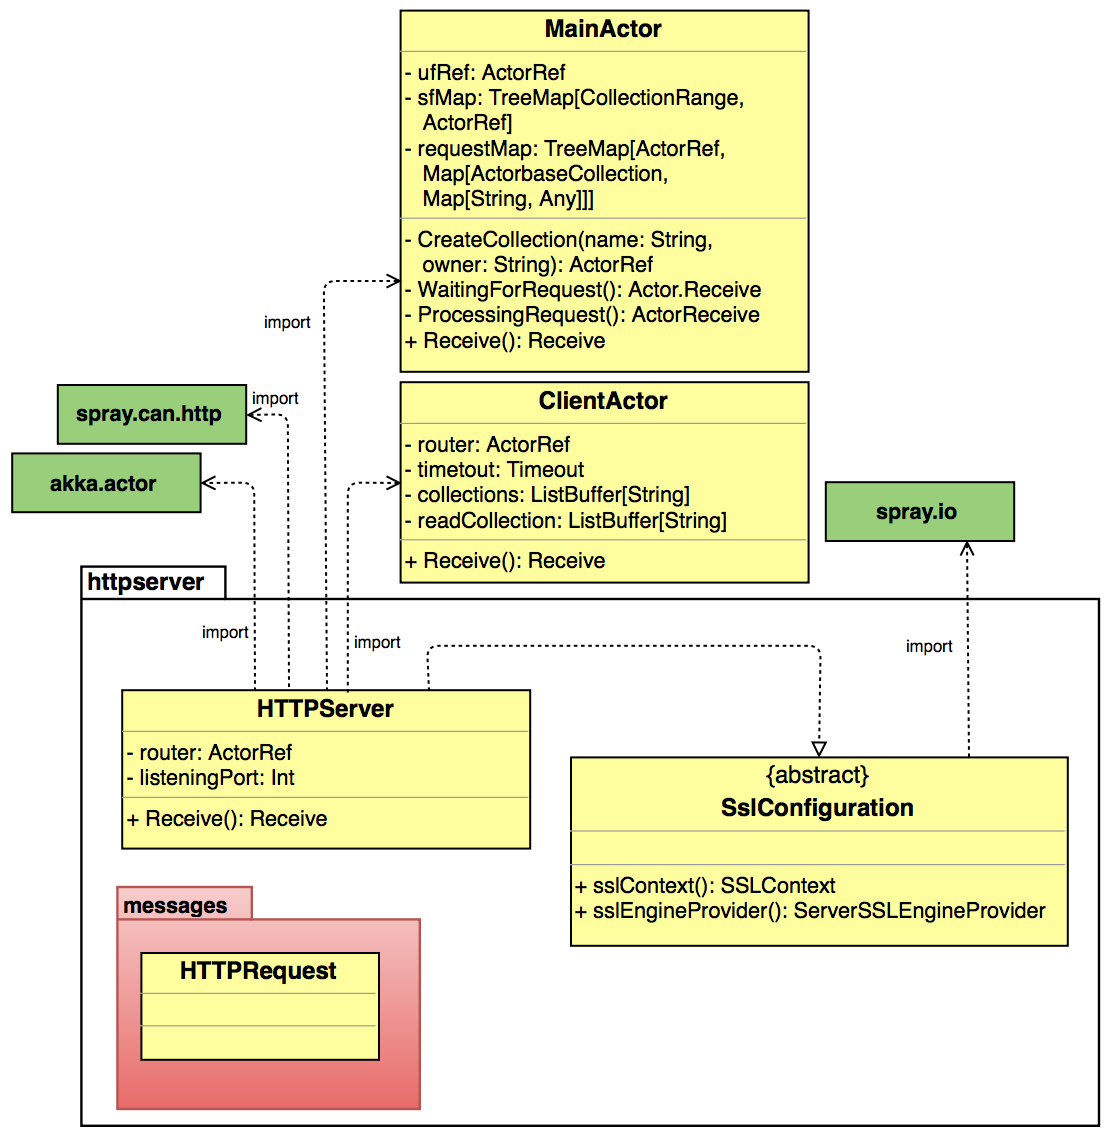
\includegraphics[width=0.5\textwidth,keepaspectratio]{RQ/httpserver.png}
    \caption{httpserver, visione generale del package}
  \end{center}
\end{figure}

\subsubsection{Descrizione}
\gloss{Package} per l'\gloss{attore} con cui si interfaccerà il \gloss{driver} per la connessione iniziale.

\subsubsection{Package contenuti}
\begin{itemize}
\item \hyperref[sec:actorbase::actorsystem::httpserver::messages]{actorbase::actorsystem::httpserver::messages}.
\end{itemize}

\subsubsection{Interazioni con altre componenti}
\begin{itemize}
\item \hyperref[sec:actorbase::actorsystem::clientactor]{actorbase::actorsystem::clientactor};
\item \hyperref[sec:actorbase::actorsystem::main]{actorbase::actorsystem::main}.
\end{itemize}

\subsubsection{Classi}

\paragraph{actorbase::actorsystem::httpserver::HTTPServer}
\label{sec:actorbase::actorsystem::httpserver::HTTPServer}

\subparagraph{Descrizione}
Classe che rappresenta l'\gloss{attore} con cui si interfaccia il \gloss{driver} per
istanziare la connessione.

\subparagraph{Utilizzo}

Questo \gloss{attore} riceve la richiesta di connessione da
\hyperref[sec:actorbase::driver::client::ActorbaseClient]{ActorbaseClient}
e si occupa di associare al \gloss{client} un \gloss{attore} di tipo
\hyperref[sec:actorbase::actorsystem::clientactor::ClientActor]{ClientActor}
per continuare le comunicazioni.

\subparagraph{Classi ereditate}
\begin{itemize}
\item \hyperref[sec:actorbase::actorsystem::httpserver::SslConfiguration]{actorbase::actorsystem::httpserver::SslConfiguration};
\item akka::actor::Actor.
\end{itemize}

\subsubsection{Interazioni con altre componenti}
\begin{itemize}
\item \hyperref[sec:actorbase::actorsystem::clientactor::ClientActor]{actorbase::actorsystem::clientactor::ClientActor};
\item \hyperref[sec:actorbase::actorsystem::main::Main]{actorbase::actorsystem::main::Main}.
\end{itemize}

\paragraph{actorbase::actorsystem::httpserver::SslConfiguration}
\label{sec:actorbase::actorsystem::httpserver::SslConfiguration}

\subparagraph{Descrizione}
Classe che contiene metodi di utilità per applicare algoritmi di crittografia
ssl.

\subparagraph{Utilizzo}
Questa classe verrà utilizzata per applicare la crittografia SSL.

%%%%%%%%%%%%%%%%%%%%%%%%%%%%%%%%%%%%%%%%%%%%%%%%%%%%%%%%%%%%%%%%%%%%%%%%%
%%%%%%%%%%%%%%%%%%%%%%%%%%%%%%%%%%%%%%%%%%%%%%%%%%%%%%%%%%%%%%%%%%%%%%%%%
%%%%%%%%%%%%%%%%%%%%%%%%%%%%%%%%%%%%%%%%%%%%%%%%%%%%%%%%%%%%%%%%%%%%%%%%%

\subsection{actorbase::actorsystem::warehouseman} %TODO DA FARE
\label{sec:actorbase::actorsystem::warehouseman}

\begin{figure}[H]
  \begin{center}
    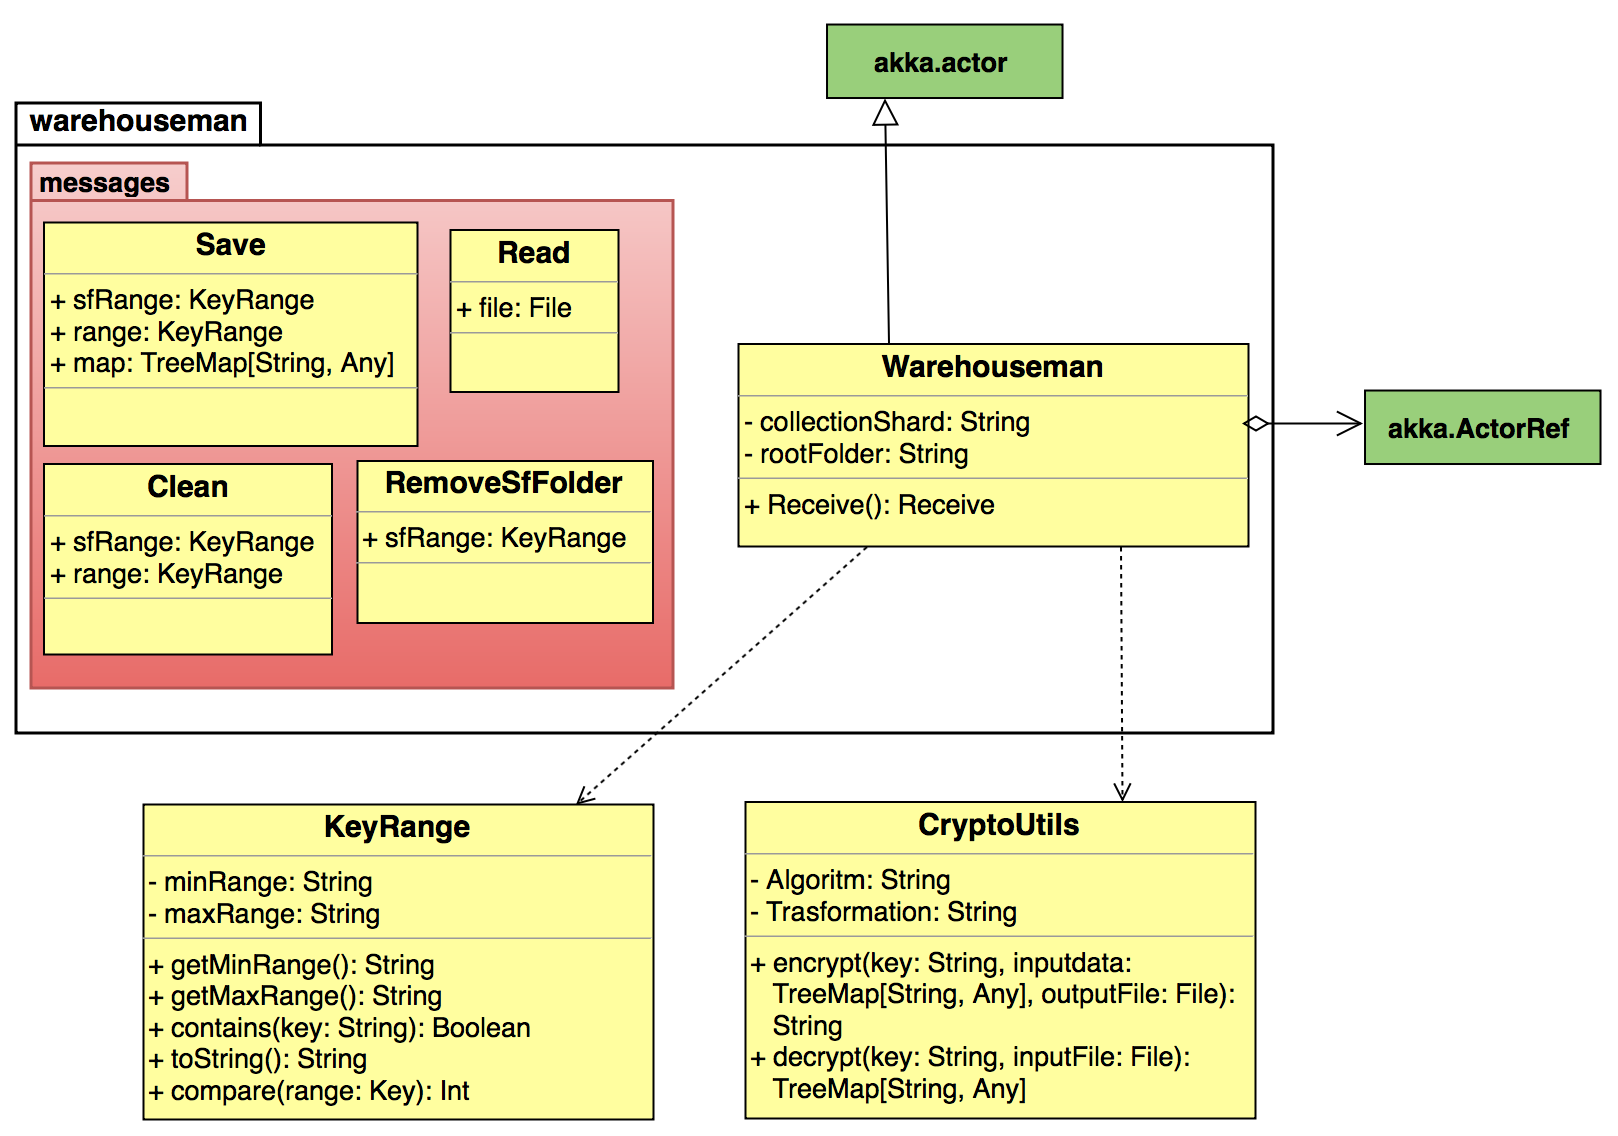
\includegraphics[width=1.0\textwidth,keepaspectratio]{RQ/Warehouseman.png}
    \caption{warehouseman, visione generale del package}
  \end{center}
\end{figure}

\subsubsection{Descrizione}

\gloss{Package} che rappresenta l'\gloss{attore} che si occuperà della
\gloss{persistenza} su disco dei dati.

\subsubsection{Package contenuti}

\begin{itemize}

\item \hyperref[sec:actorbase::actorsystem::warehouseman::messages]{actorbase::actorsystem::warehouseman::messages}.

\end{itemize}

\subsubsection{Interazioni con altre componenti}
\begin{itemize}
\item \hyperref[sec:actorbase::actorsystem::utils]{actorbase::actorsystem::utils};
\item \hyperref[sec:actorbase::actorsystem::storekeeper]{actorbase::actorsystem::storekeeper};
\item \hyperref[sec:actorbase::actorsystem::storefinder]{actorbase::actorsystem::storefinder}.
\end{itemize}

\subsubsection{Classi}

\paragraph{actorbase::actorsystem::warehouseman::Warehouseman}
\label{sec:actorbase::actorsystem::warehouseman::Warehouseman}

\subparagraph{Descrizione}
Classe che rappresenta un \gloss{attore} di tipo \gloss{Warehouseman}.

\subparagraph{Utilizzo}
Questa classe viene utilizzata per effettuare il salvataggio su filesystem del
\gloss{database} e per caricare i dati da filesystem.

\subparagraph{Classi ereditate}
\begin{itemize}
\item akka::actor::Actor.
\end{itemize}

\subparagraph{Interazioni con altre classi}
\begin{itemize}
\item \hyperref[sec:actorbase::actorsystem::utils::CryptoUtils]{actorbase::actorsystem::CryptoUtils};
\item \hyperref[sec:actorbase::actorsystem::utils::KeyRange]{actorbase::actorsystem::utils::KeyRange};
\item \hyperref[sec:actorbase::actorsystem::storekeeper::Storekeeper]{actorbase::actorsystem::storekeeper::Storekeeper};
\item \hyperref[sec:actorbase::actorsystem::storefinder::Storefinder]{actorbase::actorsystem::storefinder::Storefinder}.
\end{itemize}

\subsection{actorbase::actorsystem::warehouseman::messages}
\label{sec:actorbase::actorsystem::warehouseman::messages}

\begin{figure}[H]
  \begin{center}
    \includegraphics[width=0.6\textwidth,keepaspectratio]{RQ/classiDiag/messages-ware.png}
    \caption{Actorsystem: package messages del warehouseman}
  \end{center}
\end{figure}

\subsubsection{Descrizione}

\gloss{Package} che racchiude tutti i messaggi che gli attori di tipo
\gloss{Warehouseman} possono ricevere.

\subsubsection{Interazioni con altre componenti}
\begin{itemize}
\item \hyperref[sec:actorbase::actorsystem::utils]{actorbase::actorsystem::utils}.
\end{itemize}

\paragraph{actorbase::actorsystem::warehouseman::messages::Save}
\label{sec:actorbase::actorsystem::warehouseman::messages::Save}

\subparagraph{Descrizione}

Messaggio che porta al salvataggio dei dati su disco.

\subparagraph{Utilizzo}

Quando \hyperref[sec:actorbase::actorsystem::warehouseman::Warehouseman]{actorbase::actorsystem::warehouseman::Warehouseman}
riceve questo messaggio salverà i dati su disco sfruttando
\hyperref[sec:actorbase::actorsystem::serialization::SerializationContext]{actorbase::actorsystem::utils::CryptoUtils}.

\subparagraph{Interazioni con altre classi}
\begin{itemize}
\item \hyperref[sec:actorbase::actorsystem::utils::KeyRange]{actorbase::actorsystem::utils::KeyRange}.
\end{itemize}

\paragraph{actorbase::actorsystem::warehouseman::messages::Clean}
\label{sec:actorbase::actorsystem::warehouseman::messages::Clean}

\subparagraph{Descrizione}

Messaggio che porta alla cancellazione dal filesystem di alcuni dati.

\subparagraph{Utilizzo}

Quando \hyperref[sec:actorbase::actorsystem::warehouseman::Warehouseman]{actorbase::actorsystem::warehouseman::Warehouseman}
riceve questo messaggio rimuoverà i dati dal filesystem.

\subparagraph{Interazioni con altre classi}
\begin{itemize}
\item \hyperref[sec:actorbase::actorsystem::utils::KeyRange]{actorbase::actorsystem::utils::KeyRange}.
\end{itemize}

\paragraph{actorbase::actorsystem::warehouseman::messages::RemoveSfFolder}
\label{sec:actorbase::actorsystem::warehouseman::messages::RemoveSfFolder}

\subparagraph{Descrizione}

Messaggio che porta alla rimozione di una cartella da disco.

\subparagraph{Utilizzo}

Quando \hyperref[sec:actorbase::actorsystem::warehouseman::Warehouseman]{actorbase::actorsystem::warehouseman::Warehouseman}
riceve questo messaggio rimuoverà i dati da disco.

\subparagraph{Interazioni con altre classi}
\begin{itemize}
\item \hyperref[sec:actorbase::actorsystem::utils::KeyRange]{actorbase::actorsystem::utils::KeyRange}.
\end{itemize}

\paragraph{actorbase::actorsystem::warehouseman::messages::Read}
\label{sec:actorbase::actorsystem::warehouseman::messages::Read}

\subparagraph{Descrizione}

Messaggio che porta alla lettura di dati da disco.

\subparagraph{Utilizzo}

Quando \hyperref[sec:actorbase::actorsystem::warehouseman::Warehouseman]{actorbase::actorsystem::warehouseman::Warehouseman}
riceve questo messaggio leggerà i dati da disco sfruttando
\hyperref[sec:actorbase::actorsystem::utils::CryptoUtils]{actorbase::actorsystem::utils::CryptoUtils}.

%%%%%%%%%%%%%%%%%%%%%%%%%%%%%%%%%%%%%%%%%%%%%%%%%%%%%%%%%%%%%%%%%%%%%%%%%
%%%%%%%%%%%%%%%%%%%%%%%%%%%%%%%%%%%%%%%%%%%%%%%%%%%%%%%%%%%%%%%%%%%%%%%%%
%%%%%%%%%%%%%%%%%%%%%%%%%%%%%%%%%%%%%%%%%%%%%%%%%%%%%%%%%%%%%%%%%%%%%%%%%

\subsection{actorbase::actorsystem::main} %TODO DA controllare e finire
\label{sec:actorbase::actorsystem::main}

\begin{figure}[H]
  \begin{center}
    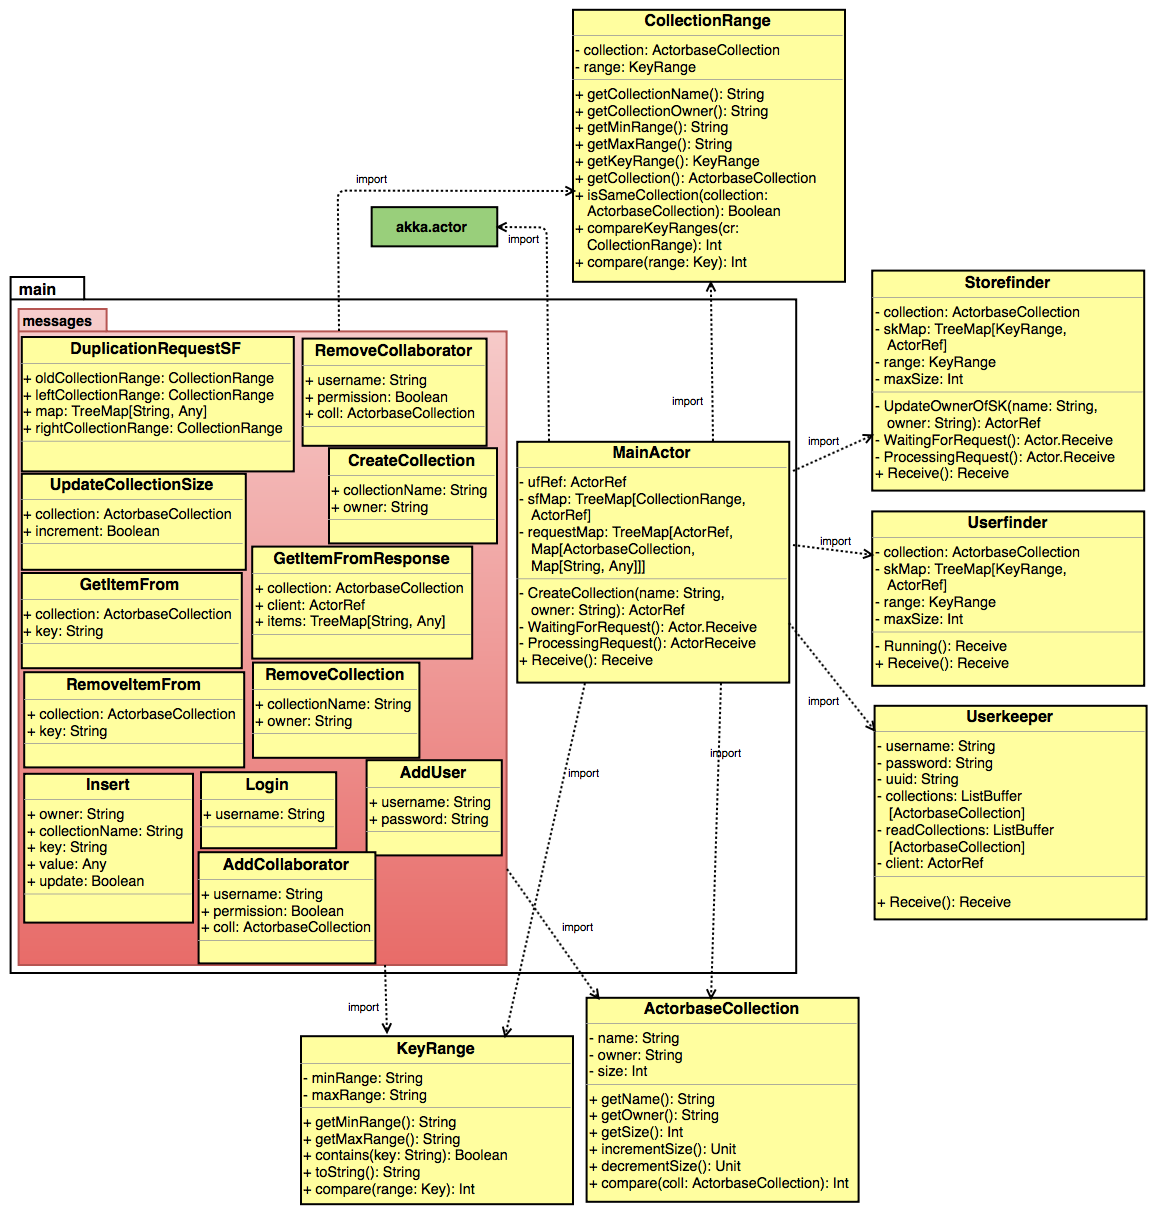
\includegraphics[width=0.8\textwidth,keepaspectratio]{RQ/Main.png}
    \caption{Package dell'attore di tipo Main}
  \end{center}
\end{figure}

\subsubsection{Descrizione}
\gloss{Package} che rappresenta l'\gloss{attore} che si occuperà di gestire le
richieste al \gloss{server}.

\subsubsection{Package contenuti}
\begin{itemize}
\item \hyperref[sec:actorbase::actorsystem::main::messages]{actorbase::actorsystem::main::messages}.
\end{itemize}

\subsubsection{Interazioni con altre componenti}
\begin{itemize}
\item \hyperref[sec:actorbase::actorsystem::httpserver]{actorbase::actorsystem::httpserver};
\item \hyperref[sec:actorbase::actorsystem::utils]{actorbase::actorsystem::utils};
\item \hyperref[sec:actorbase::actorsystem::storefinder]{actorbase::actorsystem::storefinder};
\item \hyperref[sec:actorbase::actorsystem::userkeeper]{actorbase::actorsystem::userkeeper};
\item \hyperref[sec:actorbase::actorsystem::userfinder]{actorbase::actorsystem::userfinder}.
\end{itemize}

\subsubsection{Classi}

\paragraph{actorbase::actorsystem::main::Main}
\label{sec:actorbase::actorsystem::main::Main}

\subparagraph{Descrizione}
Classe che rappresenta un \gloss{attore} di tipo \gloss{Main}.

\subparagraph{Utilizzo}
Questa classe viene utilizzata per gestire le richieste ricevute al
\gloss{server}.

\subparagraph{Classi ereditate}
\begin{itemize}
\item akka::actor::Actor.
\end{itemize}

\subparagraph{Interazioni con altre classi}
\begin{itemize}
\item \hyperref[sec:actorbase::actorsystem::httpserver::HTTPServer]{actorbase::actorsystem::httpserver::HTTPServer};
\item \hyperref[sec:actorbase::actorsystem::utils::KeyRange]{actorbase::actorsystem::utils::KeyRange};
\item \hyperref[sec:actorbase::actorsystem::utils::CollectionRange]{actorbase::actorsystem::utils::CollectionRange};
\item \hyperref[sec:actorbase::actorsystem::utils::ActorbaseCollection]{actorbase::actorsystem::utils::ActorbaseCollection};
\item \hyperref[sec:actorbase::actorsystem::storefinder::Storefinder]{actorbase::actorsystem::storefinder::Storefinder};
\item \hyperref[sec:actorbase::actorsystem::userkeeper::Userkeeper]{actorbase::actorsystem::userkeeper::Userkeeper};
\item \hyperref[sec:actorbase::actorsystem::userfinder::Userfinder]{actorbase::actorsystem::userfinder::Userfinder}.
\end{itemize}

\subsection{actorbase::actorsystem::main::messages}
\label{sec:actorbase::actorsystem::main::messages}

\begin{figure}[H]
  \begin{center}
    \includegraphics[width=0.6\textwidth,keepaspectratio]{RQ/classiDiag/messages-main.png}
    \caption{Actorsystem: package messages del main}
  \end{center}
\end{figure}

\subsubsection{Descrizione}
\gloss{Package} che racchiude tutti i messaggi che gli attori di tipo
\gloss{Main} possono ricevere.

\subsubsection{Interazioni con altre componenti}
\begin{itemize}
\item \hyperref[sec:actorbase::actorsystem::utils]{actorbase::actorsystem::utils}.
\end{itemize}

\subsubsection{Classi}

\paragraph{actorbase::actorsystem::main::messages::AddUser}
\label{sec:actorbase::actorsystem::main::messages::AddUser}

\subparagraph{Descrizione}
Messaggio che porta alla creazione di un \gloss{utente}.\\Viene ricevuto
quando un amministratore di actorbase aggiunge un utente al sistema.

\subparagraph{Utilizzo}
Quando \hyperref[sec:actorbase::actorsystem::main::Main]{actorbase::actorsystem::main::Main}
riceve questo messaggio inoltra la richiesta di aggiunta utente allo
Userfinder di cui ha riferimento.

\paragraph{actorbase::actorsystem::main::messages::Login}
\label{sec:actorbase::actorsystem::main::messages::Login}

\subparagraph{Descrizione}
Messaggio che indica una richiesta di autenticazione al sistema.

\subparagraph{Utilizzo}
Quando \hyperref[sec:actorbase::actorsystem::main::Main]{actorbase::actorsystem::main::Main}
riceve questo messaggio manderà un messaggio di tipo GetPasswordOf
all'attore di tipo \hyperref[sec:actorbase::actorsystem::userfinder::Userfinder]{Userfinder} di cui ha riferimento.

\paragraph{actorbase::actorsystem::main::messages::Insert}
\label{sec:actorbase::actorsystem::main::messages::Insert}

\subparagraph{Descrizione}
Messaggio che indica una richiesta di inserimento di un item.

\subparagraph{Utilizzo}

Quando \hyperref[sec:actorbase::actorsystem::main::Main]{Main}
riceve questo messaggio inoltrerà il messaggio allo \hyperref[sec:actorbase::actorsystem::storefinder::Storefinder]{Storefinder}
che si occupa del range di chiavi che contiene la chiave inserita.

\paragraph{actorbase::actorsystem::main::messages::RemoveItemFrom}
\label{sec:actorbase::actorsystem::main::messages::RemoveItemFrom}

\subparagraph{Descrizione}
Messaggio che indica una richiesta di rimozione di un item.

\subparagraph{Utilizzo}
Quando \hyperref[sec:actorbase::actorsystem::main::Main]{Main}
riceve questo messaggio inoltrerà il messaggio allo \hyperref[sec:actorbase::actorsystem::storefinder::Storefinder]{Storefinder}
che si occupa del range di chiavi che contiene la chiave inserita.

\paragraph{actorbase::actorsystem::main::messages::GetItemFrom}
\label{sec:actorbase::actorsystem::main::messages::GetItemFrom}

\subparagraph{Descrizione}

Messaggio che indica una richiesta di ricerca di un \gloss{item} da una \gloss{collezione}.

\subparagraph{Utilizzo}

Quando \hyperref[sec:actorbase::actorsystem::main::Main]{Main}
riceve questo messaggio cercherà gli attori di tipo
\hyperref[sec:actorbase::actorsystem::storefinder::Storefinder]{Storefinder}
corrispondenti alla \gloss{collezione} su cui effettuare la ricerca
e inoltrerà lui la richiesta dell'\gloss{item} con la chiave da cercare.

\paragraph{actorbase::actorsystem::main::messages::GetItemFromResponse}
\label{sec:actorbase::actorsystem::main::messages::GetItemFromResponse}

\subparagraph{Descrizione}

Messaggio che serve per comporre l'intera collezione da restituire all'utente

\subparagraph{Utilizzo}

Quando \hyperref[sec:actorbase::actorsystem::main::Main]{Main}
riceve questo messaggio cercherà gli attori di tipo
\hyperref[sec:actorbase::actorsystem::storefinder::Storefinder]{Storefinder}
corrispondenti alla \gloss{collezione} su cui effettuare la ricerca
e inoltrerà lui la richiesta dell'\gloss{item} con la chiave da cercare.

\paragraph{actorbase::actorsystem::main::messages::CreateCollection}
\label{sec:actorbase::actorsystem::main::messages::CreateCollection}

\subparagraph{Descrizione}
Messaggio che indica una richiesta di creazione di una \gloss{collezione}.

\subparagraph{Utilizzo}
Quando \hyperref[sec:actorbase::actorsystem::main::Main]{Main}
riceve questo messaggio provvederà a creare uno \hyperref[sec:actorbase::actorsystem::storefinder::Storefinder]{Storefinder} adibito
alla gestione della collezione e aggiornerà la propria struttura dati
aggiungendo questo riferimento.

\paragraph{actorbase::actorsystem::main::messages::RemoveCollection}
\label{sec:actorbase::actorsystem::main::messages::RemoveCollection}

\subparagraph{Descrizione}
Messaggio che indica una richiesta di rimozione di una \gloss{collezione}.

\subparagraph{Utilizzo}
Quando \hyperref[sec:actorbase::actorsystem::main::Main]{Main}
riceve questo messaggio provvederà a terminare gli attori storefinder
che rappresentano la collezione da rimuovere.

\paragraph{actorbase::actorsystem::main::messages::AddContributor}
\label{sec:actorbase::actorsystem::main::messages::AddContributor}

\subparagraph{Descrizione}

Messaggio che indica una richiesta di aggiunta di un collaboratore ad una
\gloss{collezione}.

\subparagraph{Utilizzo}

Quando \hyperref[sec:actorbase::actorsystem::main::Main]{Main}
riceve questo messaggio inoltrerà la richiesta all'attore
\hyperref[sec:actorbase::actorsystem::userfinder::Userfinder]{Userfinder}.

\paragraph{actorbase::actorsystem::main::messages::RemoveContributor}
\label{sec:actorbase::actorsystem::main::messages::RemoveContributor}

\subparagraph{Descrizione}

Messaggio che indica una richiesta di rimozione di un collaboratore da una
\gloss{collezione}.

\subparagraph{Utilizzo}

Quando \hyperref[sec:actorbase::actorsystem::main::Main]{Main}
riceve questo messaggio inoltrerà la richiesta all'attore \hyperref[sec:actorbase::actorsystem::userfinder::Userfinder]{Userfinder}.

\paragraph{actorbase::actorsystem::main::messages::Ack}
\label{sec:actorbase::actorsystem::main::messages::Ack}

\subparagraph{Descrizione}

Messaggio che indica il completamento della richiesta precedente; \hyperref[sec:actorbase::actorsystem::main::Main]{Main} torna nello stato waitingForRequests.

\subparagraph{Utilizzo}

Quando \hyperref[sec:actorbase::actorsystem::main::Main]{Main}
riceve questo messaggio cambia il suo contesto passando a waitingForRequests.

\paragraph{actorbase::actorsystem::main::messages::DuplicationRequestSF}
\label{sec:actorbase::actorsystem::main::messages::DuplicateRequestSF}

\subparagraph{Descrizione}

Messaggio che indica l'avvenuto duplicamento di uno \hyperref[sec:actorbase::actorsystem::storefinder::Storefinder]{Storefinder}.

\subparagraph{Utilizzo}
Quando \hyperref[sec:actorbase::actorsystem::main::Main]{Main}
riceve questo messaggio provvederà a aggiornare la propria struttura dati
contenente la mappatura degli \hyperref[sec:actorbase::actorsystem::storefinder::Storefinder]{Storefinder}.

\subparagraph{Interazioni con altre classi}
\begin{itemize}
\item \hyperref[sec:actorbase::actorsystem::utils::KeyRange]{actorbase::actorsystem::utils::KeyRange};
\item \hyperref[sec:actorbase::actorsystem::utils::CollectionRange]{actorbase::actorsystem::utils::CollectionRange}.
\end{itemize}

\paragraph{actorbase::actorsystem::main::messages::UpdateCollectionSize}
\label{sec:actorbase::actorsystem::main::messages::UpdateCollectionSize}

\subparagraph{Descrizione}

Messaggio che incrementa il numero delle coppie chiave-valore alla collezione

\subparagraph{Utilizzo}

Quando \hyperref[sec:actorbase::actorsystem::main::Main]{Main}
riceve questo messaggio provvederà ad inoltrare allo \hyperref[sec:actorbase::actorsystem::userfinder::Userfinder]{Userfinder} l'incremento della collezione.

\subparagraph{Interazioni con altre classi}
\begin{itemize}
\item \hyperref[sec:actorbase::actorsystem::utils::ActorbaseCollection]{actorbase::actorsystem::utils::ActorbaseCollection}.
\end{itemize}

%%%%%%%%%%%%%%%%%%%%%%%%%%%%%%%%%%%%%%%%%%%%%%%%%%%%%%%%%%%%%%%%%%%%%%%%
%%%%%%%%%%%%%%%%%%%%%%%%%%%%%%%%%%%%%%%%%%%%%%%%%%%%%%%%%%%%%%%%%%%%%%%%
%%%%%%%%%%%%%%%%%%%%%%%%%%%%%%%%%%%%%%%%%%%%%%%%%%%%%%%%%%%%%%%%%%%%%%%%

\subsection{actorbase::actorsystem::userfinder} %TODO da fare qualcosa, tipo l'immagine
\label{sec:actorbase::actorsystem::userfinder}

\begin{figure}[H]
  \begin{center}
    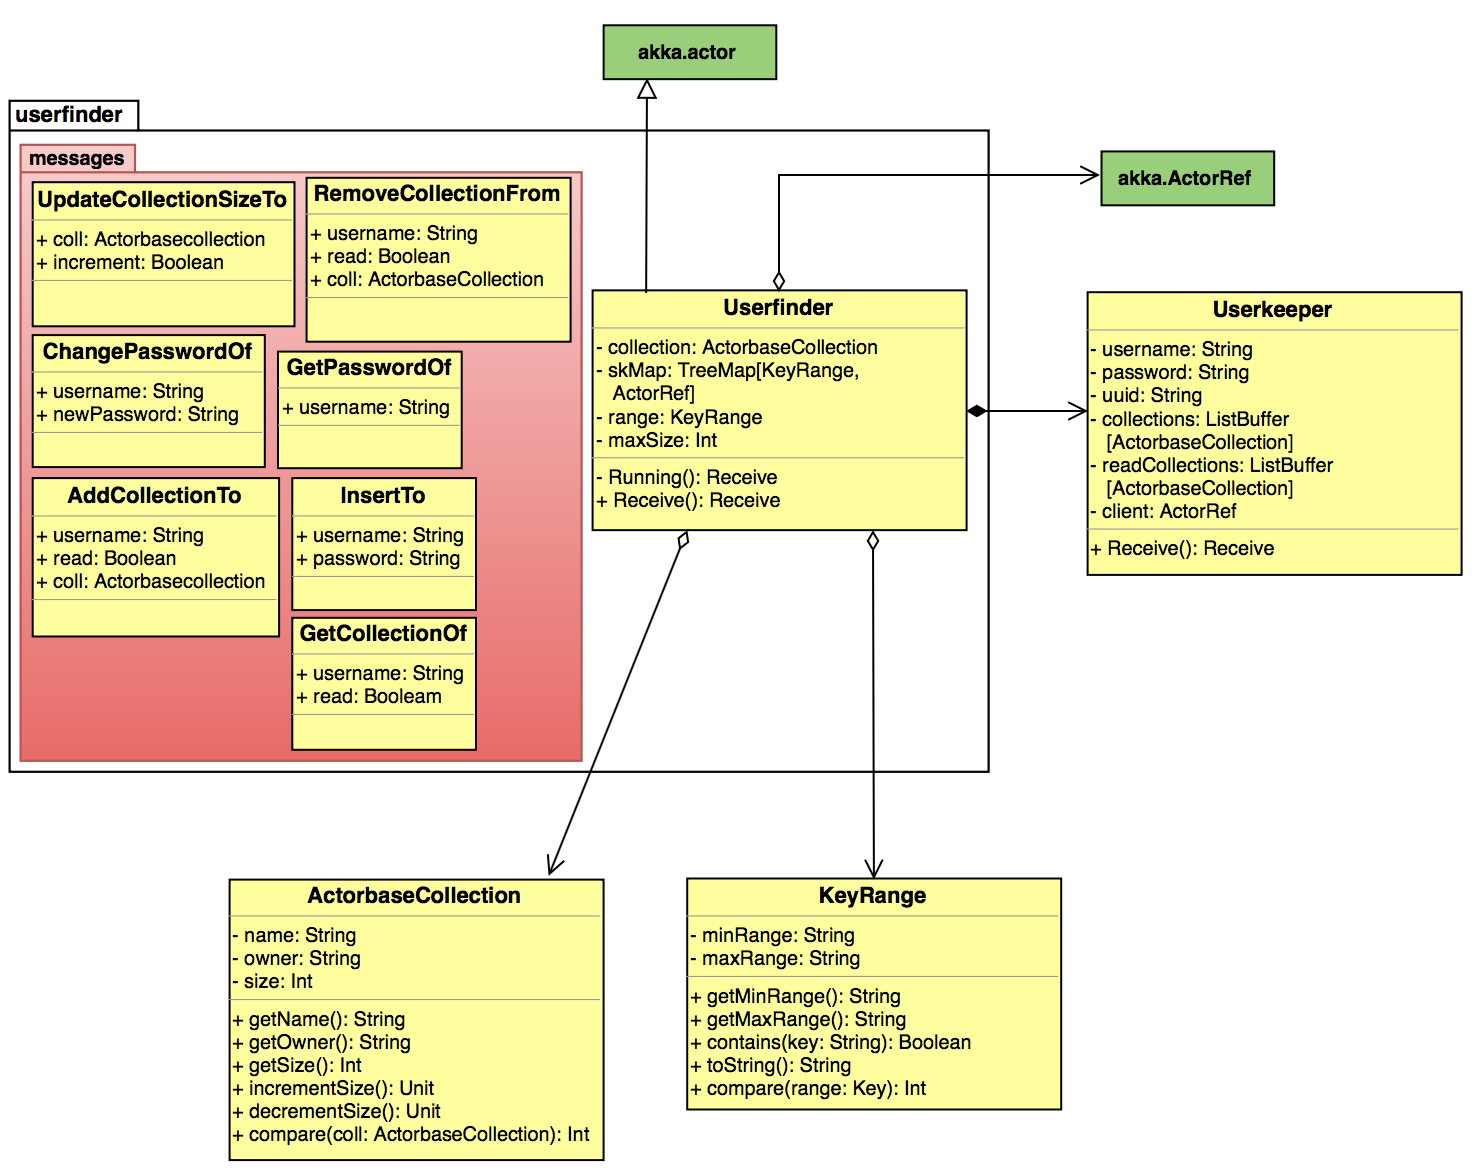
\includegraphics[width=0.8\textwidth,keepaspectratio]{RQ/userfinder.png}
    \caption{Userfinder, visione generale del package}
  \end{center}
\end{figure}

\subsubsection{Descrizione}
Classe che rappresenta un \gloss{attore} di tipo \gloss{Userfinder}.

\subsubsection{Package contenuti}
\begin{itemize}
\item \hyperref[sec:actorbase::actorsystem::userfinder::messages]{actorbase::actorsystem::userfinder::messages}.
\end{itemize}

\subsubsection{Interazioni con altre componenti}
\begin{itemize}
\item \hyperref[sec:actorbase::actorsystem::main]{actorbase::actorsystem::main};
\item \hyperref[sec:actorbase::actorsystem::utils]{actorbase::actorsystem::utils};
\item \hyperref[sec:actorbase::actorsystem::userkeeper]{actorbase::actorsystem::userkeeper}.
\end{itemize}

\subsubsection{Classi}

\paragraph{actorbase::actorsystem::userfinder::Userfinder}
\label{sec:actorbase::actorsystem::userfinder::Userfinder}

\subparagraph{Descrizione}
Classe che rappresenta un \gloss{attore} di tipo \gloss{Userfinder}.

\subparagraph{Utilizzo}
Questa classe viene utilizzata per tener traccia degli attori di tipo
\hyperref[sec:actorbase::actorsystem::userkeeper::Userkeeper]{actorbase::actorsystem::userkeeper::Userkeeper}.

\subparagraph{Classi ereditate}
\begin{itemize}
\item akka::actor::Actor.
\end{itemize}

\subparagraph{Interazioni con altre classi}
\begin{itemize}
\item \hyperref[sec:actorbase::actorsystem::main::Main]{actorbase::actorsystem::main::Main};
\item \hyperref[sec:actorbase::actorsystem::utils::KeyRange]{actorbase::actorsystem::utils::KeyRange};
\item \hyperref[sec:actorbase::actorsystem::utils::ActorbaseCollection]{actorbase::actorsystem::utils::ActorbaseCollection};
\item \hyperref[sec:actorbase::actorsystem::userkeeper::Userkeeper]{actorbase::actorsystem::userkeeper::Userkeeper}.
\end{itemize}

\subsection{actorbase::actorsystem::userfinder::messages}
\label{sec:actorbase::actorsystem::userfinder::messages}

\begin{figure}[H]
  \begin{center}
    \includegraphics[width=0.6\textwidth,keepaspectratio]{RQ/classiDiag/messages-uf.png}
    \caption{Actorsystem: package messages dello userfinder}
  \end{center}
\end{figure}

\subsubsection{Descrizione}
\gloss{Package} che contiene tutti i messaggi che possono essere ricevuti da
\hyperref[sec:actorbase::actorsystem::userfinder::Userfinder]{actorbase::actorsystem::userfinder::Userfinder}.


\subsubsection{Interazioni con altre componenti}
\begin{itemize}
\item \hyperref[sec:actorbase::actorsystem::utils]{actorbase::actorsystem::utils}.
\end{itemize}

\subsubsection{Classi}

\paragraph{actorbase::actorsystem::userfinder::messages::GetPasswordOf}
\label{sec:actorbase::actorsystem::userfinder::messages::GetPasswordOf}

\subparagraph{Descrizione}
Messaggio che indica la richiesta di autenticazione da parte di un utente.\\

\subparagraph{Utilizzo}
Quando l'attore riceve questo messaggio provvederà a inoltrare la richiesta
allo \hyperref[sec:actorbase::actorsystem::userkeeper::Userkeeper]{Userkeeper}
relativo allo username ricevuto.

\paragraph{actorbase::actorsystem::userfinder::messages::InsertTo}
\label{sec:actorbase::actorsystem::userfinder::messages::InsertTo}

\subparagraph{Descrizione}
Messaggio che indica la richiesta di un aggiunta di un utente nel sistema,
corrisponde con la creazione di un attore \hyperref[sec:actorbase::actorsystem::userkeeper::Userkeeper]{actorbase::\allowbreak{}actorsystem::\allowbreak{}userkeeper::\allowbreak{}Userkeeper}.

\subparagraph{Utilizzo}
Quando l'attore riceve questo messaggio provvederà a creare un attore di tipo \hyperref[sec:actorbase::actorsystem::userkeeper::Userkeeper]{actorbase::\allowbreak{}actorsystem::\allowbreak{}userkeeper::\allowbreak{}Userkeeper}
e l'inserimento del suo riferimento nella propria struttura dati.

\paragraph{actorbase::actorsystem::userfinder::messages::GetCollectionOf}
\label{sec:actorbase::actorsystem::userfinder::messages::GetCollectionOf}

\subparagraph{Descrizione}
Messaggio che indica la necessità di tornare le collezioni con il tipo di permessi immesso di un utente.

\subparagraph{Utilizzo}
Quando l'attore riceve questo messaggio provvederà a inoltrare la richiesta all'attore di tipo \hyperref[sec:actorbase::actorsystem::userkeeper::Userkeeper]{actorbase::\allowbreak{}actorsystem::\allowbreak{}userkeeper::\allowbreak{}Userkeeper}
che rappresenta l'utente richiesto dal parametro di ingresso.

\paragraph{actorbase::actorsystem::userfinder::messages::ChangePasswordOf}
\label{sec:actorbase::actorsystem::userfinder::messages::ChangePasswordOf}

\subparagraph{Descrizione}
Messaggio che indica la richiesta di una modifica password di un utente.

\subparagraph{Utilizzo}
Quando l'attore riceve questo messaggio provvederà a inoltrare la richiesta di cambio password all'attore di tipo \hyperref[sec:actorbase::actorsystem::userkeeper::Userkeeper]{actorbase::\allowbreak{}actorsystem::\allowbreak{}userkeeper::\allowbreak{}Userkeeper}
corrispondente all'utente corretto.

\paragraph{actorbase::actorsystem::userfinder::messages::RemoveCollectionFrom}
\label{sec:actorbase::actorsystem::userfinder::messages::RemoveCollectionFrom}

\subparagraph{Descrizione}
Messaggio che indica la richiesta di rimozione di una collezione dalla struttura dati dello \hyperref[sec:actorbase::actorsystem::userkeeper::Userkeeper]{actorbase::\allowbreak{}actorsystem::\allowbreak{}userkeeper::\allowbreak{}Userkeeper} corrispondente.

\subparagraph{Utilizzo}
Quando l'attore riceve questo messaggio provvederà a inoltrare la richiesta
all'attore di tipo \hyperref[sec:actorbase::actorsystem::userkeeper::Userkeeper]{actorbase::\allowbreak{}actorsystem::\allowbreak{}userkeeper::\allowbreak{}Userkeeper}
corrispondente all'utente corretto.

\subparagraph{Interazioni con altre classi}
\begin{itemize}
\item \hyperref[sec:actorbase::actorsystem::utils::ActorbaseCollection]{actorbase::actorsystem::utils::ActorbaseCollection}.
\end{itemize}

\paragraph{actorbase::actorsystem::userfinder::messages::AddCollectionTo}
\label{sec:actorbase::actorsystem::userfinder::messages::AddCollectionTo}

\subparagraph{Descrizione}
Messaggio che indica la richiesta di un aggiunta di una collezione con i permessi inseriti ad un utente nel sistema.

\subparagraph{Utilizzo}
Quando l'attore riceve questo messaggio provvederà a inoltrare la richiesta all'attore di tipo \hyperref[sec:actorbase::actorsystem::userkeeper::Userkeeper]{actorbase::\allowbreak{}actorsystem::\allowbreak{}userkeeper::\allowbreak{}Userkeeper}
corrispondente all'utente su cui effettuare l'operazione.

\subparagraph{Interazioni con altre classi}
\begin{itemize}
\item \hyperref[sec:actorbase::actorsystem::utils::ActorbaseCollection]{actorbase::actorsystem::utils::ActorbaseCollection}.
\end{itemize}

\paragraph{actorbase::actorsystem::userfinder::messages::UpdateCollectionSizeTo}
\label{sec:actorbase::actorsystem::userfinder::messages::UpdateCollectionSizeTo}

\subparagraph{Descrizione}

Messaggio che indica la necessità di aggiornare il numero di item di una collezione.

\subparagraph{Utilizzo}

Quando \hyperref[sec:actorbase::actorsystem::userfinder::Userfinder]{actorbase::\allowbreak{}actorsystem::\allowbreak{}userfinder::\allowbreak{}Userfinder}
riceve questo messaggio provvederà ad inoltrare all'attore di tipo
\hyperref[sec:actorbase::actorsystem::userkeeper::Userkeeper]{actorbase::\allowbreak{}actorsystem::\allowbreak{}userkeeper::\allowbreak{}Userkeeper}.

\subparagraph{Interazioni con altre classi}
\begin{itemize}
\item \hyperref[sec:actorbase::actorsystem::utils::ActorbaseCollection]{actorbase::actorsystem::utils::ActorbaseCollection}.
\end{itemize}


%%%%%%%%%%%%%%%%%%%%%%%%%%%%%%%%%%%%%%%%%%%%%%%%%%%%%%%%%%%%%%%%%%%%%%%%
%%%%%%%%%%%%%%%%%%%%%%%%%%%%%%%%%%%%%%%%%%%%%%%%%%%%%%%%%%%%%%%%%%%%%%%%
%%%%%%%%%%%%%%%%%%%%%%%%%%%%%%%%%%%%%%%%%%%%%%%%%%%%%%%%%%%%%%%%%%%%%%%%

\subsection{actorbase::actorsystem::userkeeper} %TODO fatto, non so se ci sia da aggiornare qualcosa, tipo l'immagine, boh
\label{sec:actorbase::actorsystem::userkeeper}

\begin{figure}[H]
  \begin{center}
    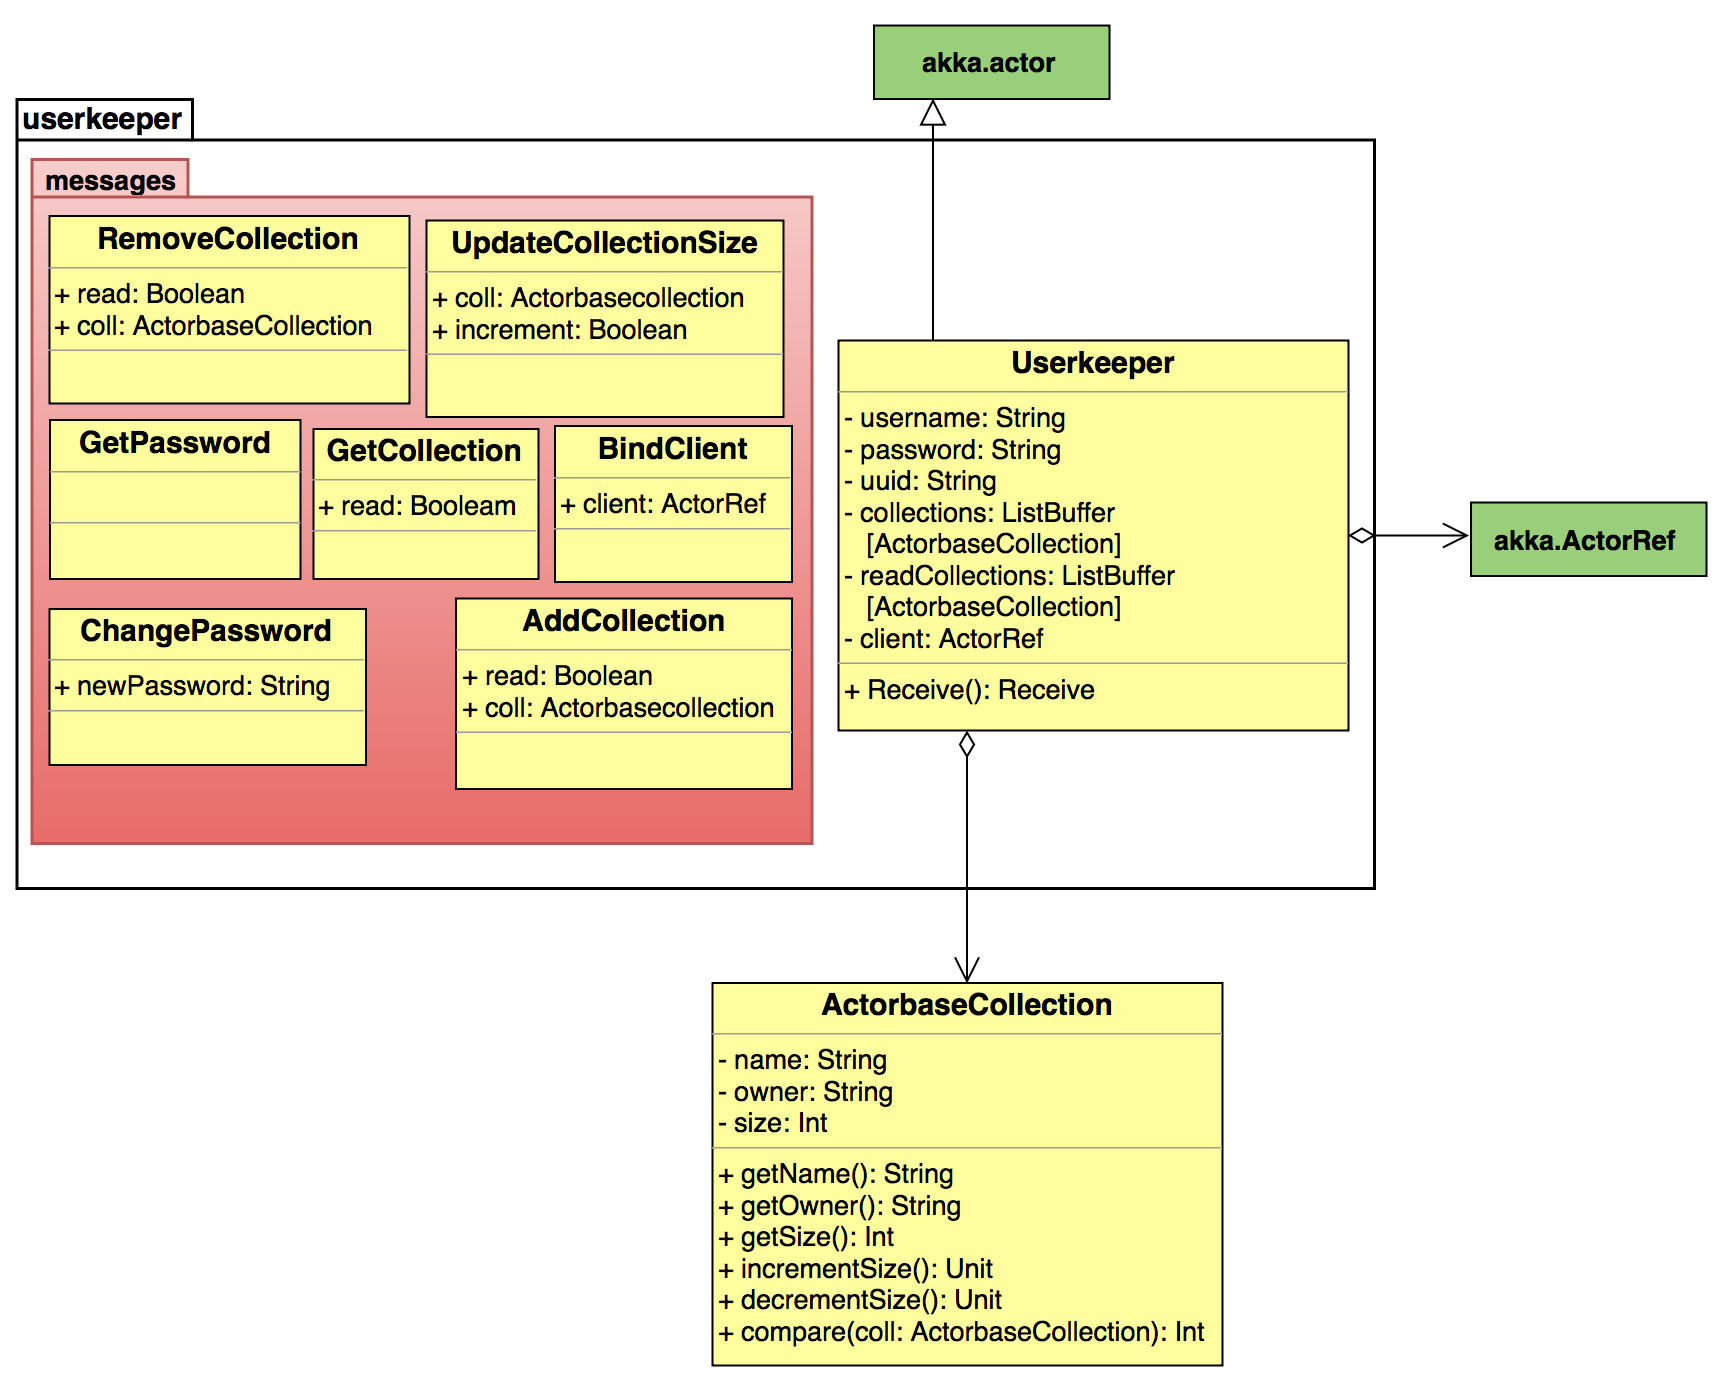
\includegraphics[width=0.8\textwidth,keepaspectratio]{RQ/userkeeper.png}
    \caption{Userkeeper, visione generale del package}
  \end{center}
\end{figure}

\subsubsection{Descrizione}
Classe che rappresenta un \gloss{attore} di tipo \gloss{Userkeeper}.

\subsubsection{Package contenuti}
\begin{itemize}
\item \hyperref[sec:actorbase::actorsystem::userkeeper::messages]{actorbase::actorsystem::userkeeper::messages}.
\end{itemize}

\subsubsection{Interazioni con altre componenti}
\begin{itemize}
\item \hyperref[sec:actorbase::actorsystem::main]{actorbase::actorsystem::main};
\item \hyperref[sec:actorbase::actorsystem::utils]{actorbase::actorsystem::utils};
\item \hyperref[sec:actorbase::actorsystem::userfinder]{actorbase::actorsystem::userfinder}.
\end{itemize}

\subsubsection{Classi}

\paragraph{actorbase::actorsystem::userkeeper::Userkeeper}
\label{sec:actorbase::actorsystem::userkeeper::Userkeeper}

\subparagraph{Descrizione}
Classe che rappresenta un \gloss{attore} di tipo \gloss{Userkeeper}.

\subparagraph{Utilizzo}
Questa classe viene utilizzata per salvare gli utenti e i loro dati nel \gloss{database}.

\subparagraph{Classi ereditate}
\begin{itemize}
\item akka::actor::Actor.
\end{itemize}

\subparagraph{Interazioni con altre classi}
\begin{itemize}
\item \hyperref[sec:actorbase::actorsystem::main::Main]{actorbase::actorsystem::main::Main};
\item \hyperref[sec:actorbase::actorsystem::utils::ActorbaseCollection]{actorbase::actorsystem::utils::ActorbaseCollection};
\item \hyperref[sec:actorbase::actorsystem::userfinder::Userfinder]{actorbase::actorsystem::userfinder::Userfinder}.
\end{itemize}

\subsection{actorbase::actorsystem::userkeeper::messages}
\label{sec:actorbase::actorsystem::userkeeper::messages}

\begin{figure}[H]
  \begin{center}
    \includegraphics[width=0.6\textwidth,keepaspectratio]{RQ/classiDiag/messages-uk.png}
    \caption{Actorsystem: package messages dello userkeepern}
  \end{center}
\end{figure}

\subsubsection{Descrizione}

\gloss{Package} che contiene tutti i messaggi che possono essere ricevuti da
\hyperref[sec:actorbase::actorsystem::userkeeper::Userkeeper]{actorbase::actorsystem::userkeeper::Userkeeper}.

\subsubsection{Interazioni con altre componenti}
\begin{itemize}
\item \hyperref[sec:actorbase::actorsystem::utils]{actorbase::actorsystem::utils}.
\end{itemize}

\subsubsection{Classi}

\paragraph{actorbase::actorsystem::userkeeper::messages::GetCollections}
\label{sec:actorbase::actorsystem::userkeeper::messages::GetCollections}

\subparagraph{Descrizione}
Messaggio che indica la richiesta della lista di \gloss{collezioni} di cui
l'utente ha permessi in lettura e scrittura.

\subparagraph{Utilizzo}
Quando \hyperref[sec:actorbase::actorsystem::userkeeper::Userkeeper]{actorbase::\allowbreak{}actorsystem::\allowbreak{}userkeeper::\allowbreak{}Userkeeper}
riceve questo messaggio provvederà a restituire all'\gloss{attore} di tipo
\hyperref[sec:actorbase::actorsystem::clientactor::ClientActor]{actorbase::\allowbreak{}actorsystem::\allowbreak{}clientactor::\allowbreak{}ClientActor}
la lista di \gloss{collezioni} di cui l'utente ha permessi in lettura
e scrittura.

\paragraph{actorbase::actorsystem::userkeeper::messages::ChangePassword}
\label{sec:actorbase::actorsystem::userkeeper::messages::ChangePassword}

\subparagraph{Descrizione}
Messaggio che indica la richiesta di cambiamento della password.

\subparagraph{Utilizzo}
Quando \hyperref[sec:actorbase::actorsystem::userkeeper::Userkeeper]{actorbase::\allowbreak{}actorsystem::\allowbreak{}userkeeper::\allowbreak{}Userkeeper}
riceve questo messaggio provvederà a modificare la password dell'utente.


\paragraph{actorbase::actorsystem::userkeeper::messages::GetPassword}
\label{sec:actorbase::actorsystem::userkeeper::messages::GetPassword}

\subparagraph{Descrizione}

Messaggio che indica la richiesta della password.

\subparagraph{Utilizzo}

Quando \hyperref[sec:actorbase::actorsystem::userkeeper::Userkeeper]{actorbase::\allowbreak{}actorsystem::\allowbreak{}userkeeper::\allowbreak{}Userkeeper}
riceve questo messaggio provvederà a inviare la password all'\gloss{attore} di tipo
\hyperref[sec:actorbase::actorsystem::clientactor::ClientActor]{actorbase::\allowbreak{}actorsystem::\allowbreak{}clientactor::\allowbreak{}ClientActor}.

\paragraph{actorbase::actorsystem::userkeeper::messages::RemoveCollection}
\label{sec:actorbase::actorsystem::userkeeper::messages::RemoveCollection}

\subparagraph{Descrizione}

Messaggio che indica la richiesta di rimozione di una \gloss{collezione} dalla
lista contenente le \gloss{collezioni} di cui l'utente ha permessi in lettura
o in scrittura.

\subparagraph{Utilizzo}

Quando \hyperref[sec:actorbase::actorsystem::userkeeper::Userkeeper]{actorbase::\allowbreak{}actorsystem::\allowbreak{}userkeeper::\allowbreak{}Userkeeper}
riceve questo messaggio provvederà a rimuovere la \gloss{collezione} desiderata
dalla lista contenente le \gloss{collezioni} di cui l'utente ha permessi in
lettura o in scrittura.

\subparagraph{Interazioni con altre classi}
\begin{itemize}
\item \hyperref[sec:actorbase::actorsystem::utils::ActorbaseCollection]{actorbase::actorsystem::utils::ActorbaseCollection}.
\end{itemize}

\paragraph{actorbase::actorsystem::userkeeper::messages::AddCollection}
\label{sec:actorbase::actorsystem::userkeeper::messages::AddCollection}

\subparagraph{Descrizione}

Messaggio che indica la richiesta di aggiunta di una \gloss{collezione} dalla
lista contenente le \gloss{collezioni} di cui l'utente ha permessi in lettura
o in lettura e scrittura.

\subparagraph{Utilizzo}

Quando \hyperref[sec:actorbase::actorsystem::userkeeper::Userkeeper]{actorbase::\allowbreak{}actorsystem::\allowbreak{}userkeeper::\allowbreak{}Userkeeper}
riceve questo messaggio provvederà ad aggiungere la \gloss{collezione} desiderata
dalla lista contenente le \gloss{collezioni} di cui l'utente ha permessi in
lettura o in lettura e scrittura.

\subparagraph{Interazioni con altre classi}
\begin{itemize}
\item \hyperref[sec:actorbase::actorsystem::utils::ActorbaseCollection]{actorbase::actorsystem::utils::ActorbaseCollection}.
\end{itemize}

\paragraph{actorbase::actorsystem::userkeeper::messages::BindClient}
\label{sec:actorbase::actorsystem::userkeeper::messages::BindClient}

\subparagraph{Descrizione}

Messaggio che indica la richiesta di collegamento con un \gloss{ClientActor}.

\subparagraph{Utilizzo}

Quando \hyperref[sec:actorbase::actorsystem::userkeeper::Userkeeper]{actorbase::\allowbreak{}actorsystem::\allowbreak{}userkeeper::\allowbreak{}Userkeeper}
riceve questo messaggio provvederà a salvarsi il riferimento dell'\gloss{attore} di tipo
\hyperref[sec:actorbase::actorsystem::clientactor::ClientActor]{actorbase::\allowbreak{}actorsystem::\allowbreak{}clientactor::\allowbreak{}ClientActor}
che ha inviato questo messaggio.

\paragraph{actorbase::actorsystem::userkeeper::messages::UpdateCollectionSize}
\label{sec:actorbase::actorsystem::userkeeper::messages::UpdateCollectionSize}

\subparagraph{Descrizione}

Messaggio che aggiorna il numero di item di una collezione.

\subparagraph{Utilizzo}

Quando \hyperref[sec:actorbase::actorsystem::userkeeper::Userkeeper]{actorbase::\allowbreak{}actorsystem::\allowbreak{}userkeeper::\allowbreak{}Userkeeper}
riceve questo messaggio provvederà ad aggiornare il contatore relativo al numero di oggetti
nella collezione.

\subparagraph{Interazioni con altre classi}
\begin{itemize}
\item \hyperref[sec:actorbase::actorsystem::utils::ActorbaseCollection]{actorbase::actorsystem::utils::ActorbaseCollection}.
\end{itemize}

%%%%%%%%%%%%%%%%%%%%%%%%%%%%%%%%%%%%%%%%%%%%%%%%%%%%%%%%%%%%%%%%%%%%%%%%
%%%%%%%%%%%%%%%%%%%%%%%%%%%%%%%%%%%%%%%%%%%%%%%%%%%%%%%%%%%%%%%%%%%%%%%%
%%%%%%%%%%%%%%%%%%%%%%%%%%%%%%%%%%%%%%%%%%%%%%%%%%%%%%%%%%%%%%%%%%%%%%%%

\subsection{actorbase::actorsystem::storefinder} %TODO DA controllare e finire
\label{sec:actorbase::actorsystem::storefinder}

\begin{figure}[H]
  \begin{center}
    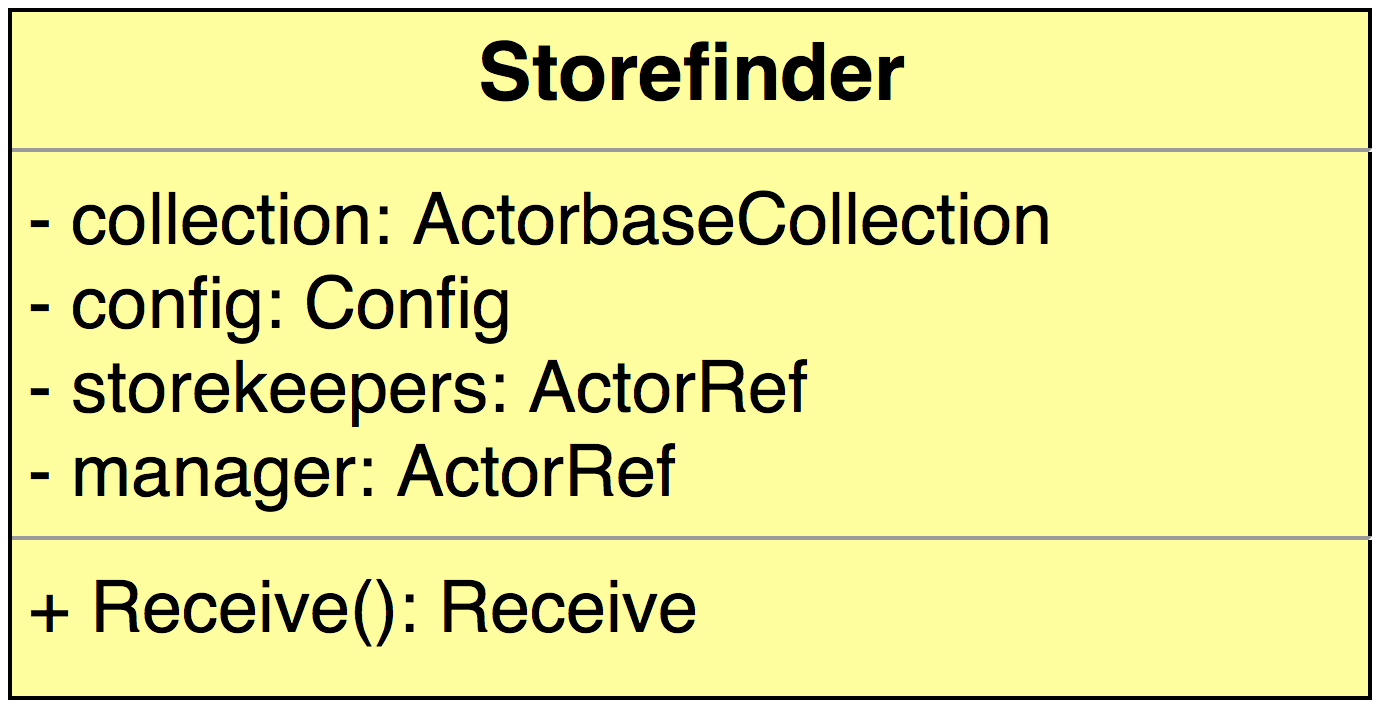
\includegraphics[width=0.8\textwidth,keepaspectratio]{RQ/storefinder.png}
    \caption{Storefinder, visione generale del package}
  \end{center}
\end{figure}

\subsubsection{Descrizione}
Classe che rappresenta un \gloss{attore} di tipo \gloss{Storefinder}.

\subsubsection{Package contenuti}
\begin{itemize}
\item \hyperref[sec:actorbase::actorsystem::storefinder::messages]{actorbase::actorsystem::storefinder::messages}.
\end{itemize}

\subsubsection{Interazioni con altre componenti}
\begin{itemize}
\item \hyperref[sec:actorbase::actorsystem::main]{actorbase::actorsystem::main};
\item \hyperref[sec:actorbase::actorsystem::utils]{actorbase::actorsystem::utils};
\item \hyperref[sec:actorbase::actorsystem::storekeeper]{actorbase::actorsystem::storekeeper};
\item \hyperref[sec:actorbase::actorsystem::warehouseman]{actorbase::actorsystem::warehouseman}.
\end{itemize}

\subsubsection{Classi}

\paragraph{actorbase::actorsystem::storefinder::Storefinder}
\label{sec:actorbase::actorsystem::storefinder::Storefinder}

\subparagraph{Descrizione}

Classe che rappresenta un \gloss{attore} di tipo \gloss{Storefinder}.

\subparagraph{Utilizzo}
Questa classe viene utilizzata per tener traccia degli attori di tipo
\hyperref[sec:actorbase::actorsystem::storekeeper::Storekeeper]{actorbase::actorsystem::storekeeper::Storekeeper}.

\subparagraph{Classi ereditate}

\begin{itemize}

\item akka::actor::Actor.

\end{itemize}

\subparagraph{Interazioni con altre classi}
\begin{itemize}
\item \hyperref[sec:actorbase::actorsystem::main::Main]{actorbase::actorsystem::main::Main};
\item \hyperref[sec:actorbase::actorsystem::utils::ActorbaseCollection]{actorbase::actorsystem::utils::ActorbaseCollection};
\item \hyperref[sec:actorbase::actorsystem::utils::KeyRange]{actorbase::actorsystem::utils::KeyRange};
\item \hyperref[sec:actorbase::actorsystem::utils::CollectionRange]{actorbase::actorsystem::utils::CollectionRange};
\item \hyperref[sec:actorbase::actorsystem::storekeeper::Storekeeper]{actorbase::actorsystem::storekeeper::Storekeeper};
\item \hyperref[sec:actorbase::actorsystem::warehouseman::Warehouseman]{actorbase::actorsystem::warehouseman::Warehouseman}.
\end{itemize}

\subsection{actorbase::actorsystem::storefinder::messages}
\label{sec:actorbase::actorsystem::storefinder::messages}

\begin{figure}[H]
  \begin{center}
    \includegraphics[width=0.6\textwidth,keepaspectratio]{RQ/classiDiag/messages-sf.png}
    \caption{Actorsystem: package messages dello storefinder}
  \end{center}
\end{figure}

\subsubsection{Descrizione}

\gloss{Package} che contiene tutti i messaggi che possono essere ricevuti da
\hyperref[sec:actorbase::actorsystem::storefinder::Storefinder]{actorbase::actorsystem::storefinder::Storefinder}.

\subsubsection{Interazioni con altre componenti}
\begin{itemize}
\item \hyperref[sec:actorbase::actorsystem::utils]{actorbase::actorsystem::utils}.
\end{itemize}


\subsubsection{Classi}

\paragraph{actorbase::actorsystem::storefinder::messages::DuplicationRequestSK}
\label{sec:actorbase::actorsystem::storefinder::messages::DuplicationRequestSK}

\subparagraph{Descrizione}
Messaggio atto ad aggiornare uno Storefinder a seguito di una duplicazione
di un attore di tipo Storekeeper.\\

\subparagraph{Utilizzo}
Quando \hyperref[sec:actorbase::actorsystem::storefinder::Storefinder]{actorbase::\allowbreak{}actorsystem::\allowbreak{}storefinder::\allowbreak{}Storefinder}
riceve questo messaggio provvederà ad aggiornare la sua struttura dati.\\In
particolare aggiornerà i range di chiavi contenuti dagli Storekeeper presenti
nella sua struttura dati.

\subparagraph{Interazioni con altre classi}
\begin{itemize}
\item \hyperref[sec:actorbase::actorsystem::utils::KeyRange]{actorbase::actorsystem::utils::KeyRange}.
\end{itemize}

\paragraph{actorbase::actorsystem::storefinder::messages::Ack}
\label{sec:actorbase::actorsystem::storefinder::messages::Ack}

\begin{figure}[H]
  \begin{center}
    \includegraphics[width=0.1\textwidth,keepaspectratio]{RQ/classiDiag/ack-main.png}
    \caption{Classe actorsystem::storefinder::messages::Ack}
  \end{center}
\end{figure}

\subparagraph{Descrizione}

Messaggio che indica il completamento della richiesta precedente;
\hyperref[sec:actorbase::actorsystem::storefinder::Storefinder]{Storefinder} torna nello stato waitingForRequests.

\subparagraph{Utilizzo}

Quando \hyperref[sec:actorbase::actorsystem::storefinder::Storefinder]{Storefinder}
riceve questo messaggio cambia il suo contesto panssando a waitingForRequests.

\paragraph{actorbase::actorsystem::storefinder::messages::GetItem}
\label{sec:actorbase::actorsystem::storefinder::messages::GetItem}

\subparagraph{Descrizione}

Messaggio che indica la richiesta di un \gloss{item}.

\subparagraph{Utilizzo}

Quando \hyperref[sec:actorbase::actorsystem::storefinder::Storefinder]{actorbase::\allowbreak{}actorsystem::\allowbreak{}storefinder::\allowbreak{}Storefinder}
riceve questo messaggio provvederà a inoltrare la richiesta all'\gloss{attore} di tipo
\hyperref[sec:actorbase::actorsystem::storekeeper::Storekeeper]{actorbase::\allowbreak{}actorsystem::\allowbreak{}storekeeper::\allowbreak{}Storekeeper}
che contiene l'\gloss{item} cercato.

\paragraph{actorbase::actorsystem::storefinder::messages::RemoveItem}
\label{sec:actorbase::actorsystem::storefinder::messages::RemoveItem}

\subparagraph{Descrizione}

Messaggio che indica la richiesta di rimozione di un \gloss{item}.

\subparagraph{Utilizzo}

Quando \hyperref[sec:actorbase::actorsystem::storefinder::Storefinder]{actorbase::\allowbreak{}actorsystem::\allowbreak{}storefinder::\allowbreak{}Storefinder}
riceve questo messaggio provvederà a inoltrare la richiesta all'\gloss{attore} di tipo
\hyperref[sec:actorbase::actorsystem::storekeeper::Storekeeper]{actorbase::\allowbreak{}actorsystem::\allowbreak{}storekeeper::\allowbreak{}Storekeeper}
che contiene l'\gloss{item} da rimuovere.

\paragraph{actorbase::actorsystem::storefinder::messages::Insert}
\label{sec:actorbase::actorsystem::storefinder::messages::Insert}

\subparagraph{Descrizione}

Messaggio che indica la richiesta di inserimento di un \gloss{item}.

\subparagraph{Utilizzo}

Quando \hyperref[sec:actorbase::actorsystem::storefinder::Storefinder]{actorbase::\allowbreak{}actorsystem::\allowbreak{}storefinder::\allowbreak{}Storefinder}
riceve questo messaggio provvederà a inoltrare la richiesta all'\gloss{attore} di tipo
\hyperref[sec:actorbase::actorsystem::storekeeper::Storekeeper]{actorbase::\allowbreak{}actorsystem::\allowbreak{}storekeeper::\allowbreak{}Storekeeper}
destinato a ricevere l'\gloss{item} da inserire.

\paragraph{actorbase::actorsystem::storefinder::messages::GetAllItem}
\label{sec:actorbase::actorsystem::storefinder::messages::GetAllItem}

\subparagraph{Descrizione}

Messaggio che indica la richiesta di restituzione di tutti gli
\gloss{item} mappati dallo Storefinder.

\subparagraph{Utilizzo}

Quando \hyperref[sec:actorbase::actorsystem::storefinder::Storefinder]{actorbase::\allowbreak{}actorsystem::\allowbreak{}storefinder::\allowbreak{}Storefinder}
riceve questo messaggio provvederà a inoltrare la richiesta a tutti gli attori
di tipo
\hyperref[sec:actorbase::actorsystem::storekeeper::Storekeeper]{actorbase::\allowbreak{}actorsystem::\allowbreak{}storekeeper::\allowbreak{}Storekeeper}
che dovranno restituire tutti gli \gloss{items} contenuti in essi.

\paragraph{actorbase::actorsystem::storefinder::messages::GetAllItemResponse}
\label{sec:actorbase::actorsystem::storefinder::messages::GetAllItemResponse}

\subparagraph{Descrizione}

Messaggio che serve per comporre l'intera collezione da restituire all'utente

\subparagraph{Utilizzo}

Quando \hyperref[sec:actorbase::actorsystem::storefinder::Storefinder]{Storefinder}
riceve questo messaggio non farà altro che richiamare il metodo
\hyperref[sec:actorbase::actorsystem::main::messages::GetItemFromResponse]{GetItemFromResponse} del Main.

\paragraph{actorbase::actorsystem::storefinder::messages::UpdateCollectionSize}
\label{sec:actorbase::actorsystem::storefinder::messages::UpdateCollectionSize}

\subparagraph{Descrizione}

Messaggio che incrementa il numero delle coppie chiave-valore alla collezione

\subparagraph{Utilizzo}

Quando \hyperref[sec:actorbase::actorsystem::storefinder::Storefinder]{Storefinder}
riceve questo messaggio non farà altro che richiamare il metodo
\hyperref[sec:actorbase::actorsystem::main::messages::UpdateCollectionSize]{UpdateCollectionSize} del Main.

\subparagraph{Interazioni con altre classi}
\begin{itemize}
\item \hyperref[sec:actorbase::actorsystem::utils::ActorbaseCollection]{actorbase::actorsystem::utils::ActorbaseCollection}.
\end{itemize}

%%%%%%%%%%%%%%%%%%%%%%%%%%%%%%%%%%%%%%%%%%%%%%%%%%%%%%%%%%%%%%%%%%%%%%%%
%%%%%%%%%%%%%%%%%%%%%%%%%%%%%%%%%%%%%%%%%%%%%%%%%%%%%%%%%%%%%%%%%%%%%%%%
%%%%%%%%%%%%%%%%%%%%%%%%%%%%%%%%%%%%%%%%%%%%%%%%%%%%%%%%%%%%%%%%%%%%%%%%

\subsection{actorbase::actorsystem::storekeeper}
\label{sec:actorbase::actorsystem::storekeeper}

\begin{figure}[H]
  \begin{center}
    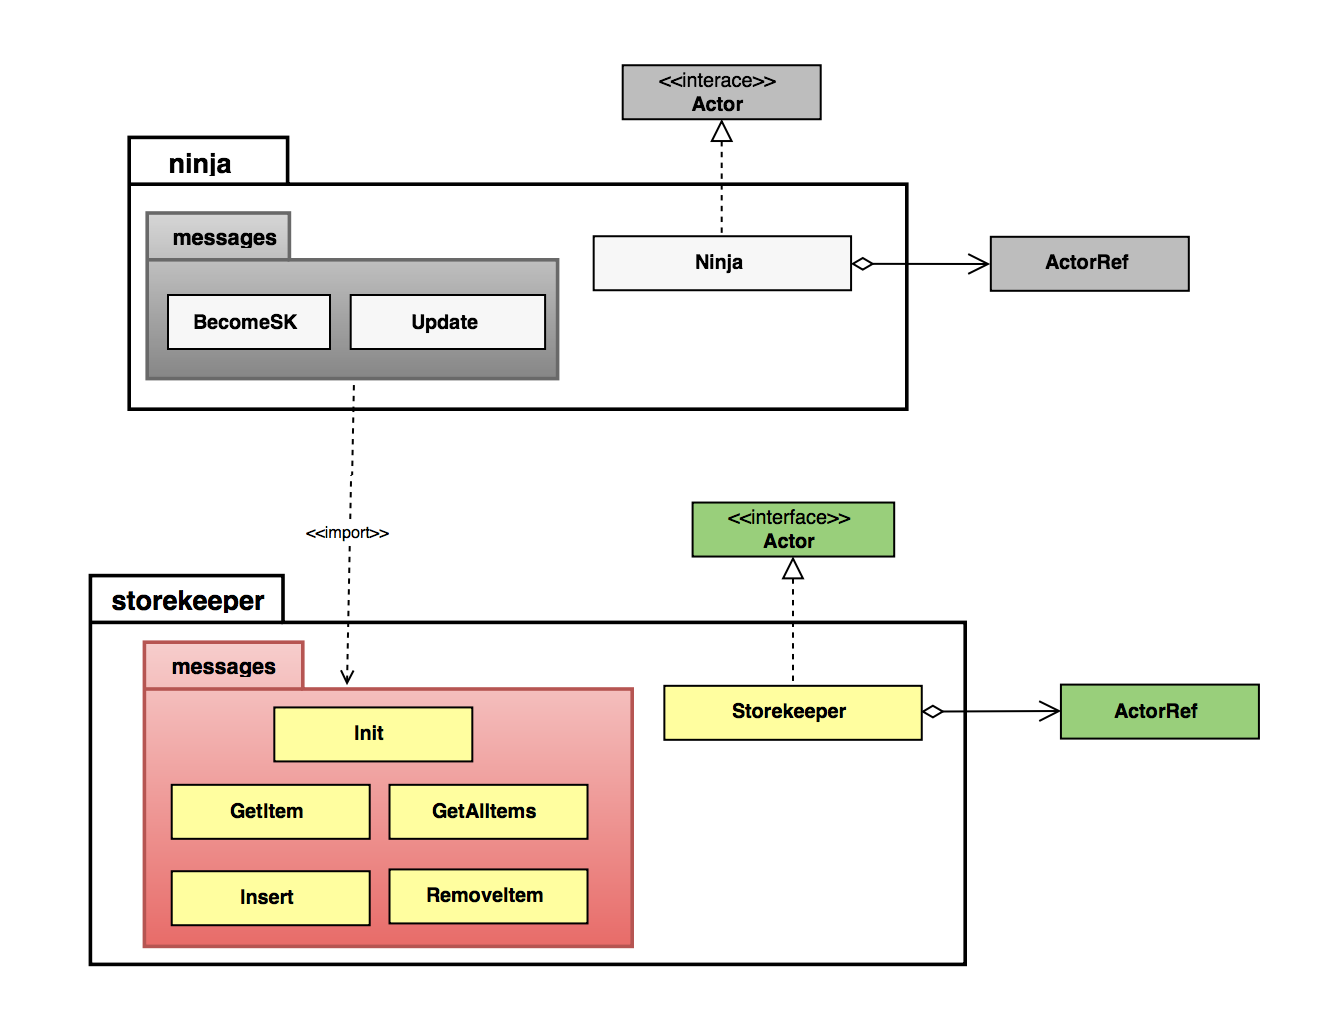
\includegraphics[width=0.8\textwidth,keepaspectratio]{RQ/Storekeeper.png}
    \caption{Storekeeper, visione generale del package}
  \end{center}
\end{figure}

\subsubsection{Descrizione}
\gloss{Package} che rappresenta l'\gloss{attore} di tipo \gloss{Storekeeper}.

\subsubsection{Package contenuti}
\begin{itemize}
\item \hyperref[sec:actorbase::actorsystem::storekeeper::messages]{actorbase::actorsystem::storekeeper::messages}.
\end{itemize}

\subsubsection{Interazioni con altre componenti}
\begin{itemize}
\item \hyperref[sec:actorbase::actorsystem::utils]{actorbase::actorsystem::utils};
\item \hyperref[sec:actorbase::actorsystem::storefinder]{actorbase::actorsystem::storefinder};
\item \hyperref[sec:actorbase::actorsystem::warehouseman]{actorbase::actorsystem::warehouseman}.
\end{itemize}

\subsubsection{Classi}

\paragraph{actorbase::actorsystem::storekeeper::Storekeeper}
\label{sec:actorbase::actorsystem::storekeeper::Storekeeper}

\subparagraph{Descrizione}
Classe che rappresenta un \gloss{attore} di tipo \gloss{Storekeeper}.

\subparagraph{Utilizzo}
Questa classe viene utilizzata per salvare nel \gloss{database} gli item.

\subparagraph{Classi ereditate}
\begin{itemize}
\item akka::actor::Actor.
\end{itemize}

\subparagraph{Interazioni con altre classi}
\begin{itemize}
\item \hyperref[sec:actorbase::actorsystem::utils::ActorbaseCollection]{actorbase::actorsystem::utils::ActorbaseCollection};
\item \hyperref[sec:actorbase::actorsystem::utils::KeyRange]{actorbase::actorsystem::utils::KeyRange};
\item \hyperref[sec:actorbase::actorsystem::storefinder::Storefinder]{actorbase::actorsystem::storefinder::Storefinder};
\item \hyperref[sec:actorbase::actorsystem::warehouseman::Warehouseman]{actorbase::actorsystem::warehouseman::Warehouseman}.
\end{itemize}

\subsection{actorbase::actorsystem::storekeeper::messages}
\label{sec:actorbase::actorsystem::storekeeper::messages}

\begin{figure}[H]
  \begin{center}
    \includegraphics[width=0.6\textwidth,keepaspectratio]{RQ/classiDiag/messages-sk.png}
    \caption{Actorsystem: package messages dello storekeeper}
  \end{center}
\end{figure}

\subsubsection{Descrizione}

\gloss{Package} che contiene tutti i messaggi che possono essere
ricevuti dall'\gloss{attore} di tipo
\hyperref[sec:actorbase::actorsystem::storekeeper::Storekeeper]{actorbase::\allowbreak{}actorsystem::\allowbreak{}storekeeper::\allowbreak{}Storekeeper}.

\subsubsection{Interazioni con altre componenti}
\begin{itemize}
\item \hyperref[sec:actorbase::actorsystem::utils]{actorbase::actorsystem::utils}.
\end{itemize}

\subsubsection{Classi}

\paragraph{actorbase::actorsystem::storekeeper::messages::GetItem}
\label{sec:actorbase::actorsystem::storekeeper::messages::GetItem}

\subparagraph{Descrizione}

Messaggio che richiede un \gloss{item} contenuto dall'\gloss{attore}
\gloss{Storekeeper} che lo riceve.

\subparagraph{Utilizzo}

Quando \hyperref[sec:actorbase::actorsystem::storekeeper::Storekeeper]{actorbase::actorsystem::storekeeper::Storekeeper}
riceve questo messaggio risponde mandando l'\gloss{item} cercato all'\gloss{attore} di tipo
\hyperref[sec:actorbase::actorsystem::clientactor::ClientActor]{actorbase::actorsystem::clientactor::ClientActor}
che aveva effettuato la richiesta.

\paragraph{actorbase::actorsystem::storekeeper::messages::GetAllItem}
\label{sec:actorbase::actorsystem::storekeeper::messages::GetAllItem}

\subparagraph{Descrizione}

Messaggio che richiede gli \gloss{item} contenuti dall'\gloss{attore}
\gloss{Storekeeper} che lo riceve.

\subparagraph{Utilizzo}

Quando \hyperref[sec:actorbase::actorsystem::storekeeper::Storekeeper]{actorbase::actorsystem::storekeeper::Storekeeper}
riceve questo messaggio risponde mandando gli \gloss{item} all'\gloss{attore} di tipo
\hyperref[sec:actorbase::actorsystem::clientactor::ClientActor]{actorbase::actorsystem::clientactor::ClientActor}
che aveva effettuato la richiesta.

\paragraph{actorbase::actorsystem::storekeeper::messages::Insert}
\label{sec:actorbase::actorsystem::storekeeper::messages::Insert}

\subparagraph{Descrizione}

Messaggio che richiede l'inserimento di un \gloss{item}.

\subparagraph{Utilizzo}

Quando \hyperref[sec:actorbase::actorsystem::storekeeper::Storekeeper]{actorbase::actorsystem::storekeeper::Storekeeper}
riceve questo messaggio inserisce l'\gloss{item} nel suo attributo data.

\paragraph{actorbase::actorsystem::storekeeper::messages::RemoveItem}
\label{sec:actorbase::actorsystem::storekeeper::messages::RemoveItem}

\subparagraph{Descrizione}

Messaggio che richiede la rimozione di un \gloss{item}.

\subparagraph{Utilizzo}

Quando \hyperref[sec:actorbase::actorsystem::storekeeper::Storekeeper]{actorbase::actorsystem::storekeeper::Storekeeper}
riceve questo messaggio rimuove l'\gloss{item}.

\paragraph{actorbase::actorsystem::storekeeper::messages::UpdateOwnerOfSk}
\label{sec:actorbase::actorsystem::storekeeper::messages::UpdateOwnerOfSk}

\subparagraph{Descrizione}

Messaggio che richiede l'update del campo dati che rappresenta lo \hyperref[sec:actorbase::actorsystem::storefinder::Storefinder]{Storefinder} che contiene lo \hyperref[sec:actorbase::actorsystem::storekeeper::Storekeeper]{Storekeeper} che ha ricevuto il messaggio.

\subparagraph{Utilizzo}

Quando \hyperref[sec:actorbase::actorsystem::storekeeper::Storekeeper]{Storekeeper}
riceve questo messaggio aggiorna il campo dati relativo allo \hyperref[sec:actorbase::actorsystem::storefinder::Storefinder]{Storefinder} che lo contiene.

\subparagraph{Interazioni con altre classi}
\begin{itemize}
\item \hyperref[sec:actorbase::actorsystem::utils::KeyRange]{actorbase::actorsystem::utils::KeyRange}.
\end{itemize}

\paragraph{actorbase::actorsystem::storekeeper::messages::Update}
\label{sec:actorbase::actorsystem::storekeeper::messages::Update}

\subparagraph{Descrizione}

Messaggio che richiede l'update dell'\gloss{attore} che lo riceve.

\subparagraph{Utilizzo}

Quando \hyperref[sec:actorbase::actorsystem::storekeeper::Storekeeper]{actorbase::actorsystem::storekeeper::Storekeeper}
riceve questo messaggio aggiorna gli \gloss{item} che contiene.

\paragraph{actorbase::actorsystem::storekeeper::messages::BecomeSK}
\label{sec:actorbase::actorsystem::storekeeper::messages::BecomeSK}

\subparagraph{Descrizione}

Messaggio che richiede che l'\gloss{attore} di tipo \gloss{Ninja} diventi di tipo
\gloss{Storekeeper}.

\subparagraph{Utilizzo}
Quando \hyperref[sec:actorbase::actorsystem::storekeeper::Storekeeper]{actorbase::actorsystem::storekeeper::Storekeeper}
riceve questo messaggio ed è attualmente un attore di tipo \gloss{Ninja},
esso cambia il proprio contesto e potrà ricevere tutti i messaggi
di \hyperref[sec:actorbase::actorsystem::storekeeper::messages]{actorbase::\allowbreak{}actorsystem::\allowbreak{}storekeeper::\allowbreak{}messages}
eccetto \hyperref[sec:actorbase::actorsystem::storekeeper::messages::BecomeNinja]{actorbase::\allowbreak{}actorsystem::\allowbreak{}storekeeper::\allowbreak{}messages::\allowbreak{}BecomeNinja} e
\hyperref[sec:actorbase::actorsystem::storekeeper::messages::Update]{actorbase::\allowbreak{}actorsystem::\allowbreak{}storekeeper::\allowbreak{}messages::\allowbreak{}Update}.

\paragraph{actorbase::actorsystem::storekeeper::messages::BecomeNinja}
\label{sec:actorbase::actorsystem::storekeeper::messages::BecomeNinja}

\subparagraph{Descrizione}
Messaggio che richiede che l'\gloss{attore} di tipo \gloss{Storekeeper} diventi di tipo
\gloss{Ninja}.

\subparagraph{Utilizzo}
Quando \hyperref[sec:actorbase::actorsystem::storekeeper::Storekeeper]{actorbase::actorsystem::storekeeper::Storekeeper}
riceve questo messaggio cambia il proprio contesto diventando un attore di tipo \gloss{Ninja}. Questo comporta l'accesso ai messaggi
\hyperref[sec:actorbase::actorsystem::storekeeper::messages::BecomeNinja]{actorbase::\allowbreak{}actorsystem::\allowbreak{}storekeeper::\allowbreak{}messages::\allowbreak{}BecomeNinja},
\hyperref[sec:actorbase::actorsystem::storekeeper::messages::Update]{actorbase::\allowbreak{}actorsystem::\allowbreak{}storekeeper::\allowbreak{}messages::\allowbreak{}Update}.

\paragraph{actorbase::actorsystem::storekeeper::messages::Persist}
\label{sec:actorbase::actorsystem::storekeeper::messages::Persist}

\subparagraph{Descrizione}
Messaggio che richiede che il salvataggio su disco dei dati contenuti.

\subparagraph{Utilizzo}
Quando lo \hyperref[sec:actorbase::actorsystem::storekeeper::Storekeeper]{Storekeeper}
riceve questo messaggio si occupa di mandare un messaggio al \hyperref[sec:actorbase::actorsystem::warehouseman::Warehouseman]{Warehouseman}
per il salvataggio dei propri dati su disco.


%%%%%%%%%%%%%%%%%%%%%%%%%%%%%%%%%%%%%%%%%%%%%%%%%%%%%%%%%%%%%%%%%%%%%%%%
%%%%%%%%%%%%%%%%%%%%%%%%%%%%%%%%%%%%%%%%%%%%%%%%%%%%%%%%%%%%%%%%%%%%%%%%
%%%%%%%%%%%%%%%%%%%%%%%%%%%%%%%%%%%%%%%%%%%%%%%%%%%%%%%%%%%%%%%%%%%%%%%%

\subsection{actorbase::actorsystem::manager}
\label{sec:actorbase::actorsystem::manager}

\begin{figure}[H]
  \begin{center}
    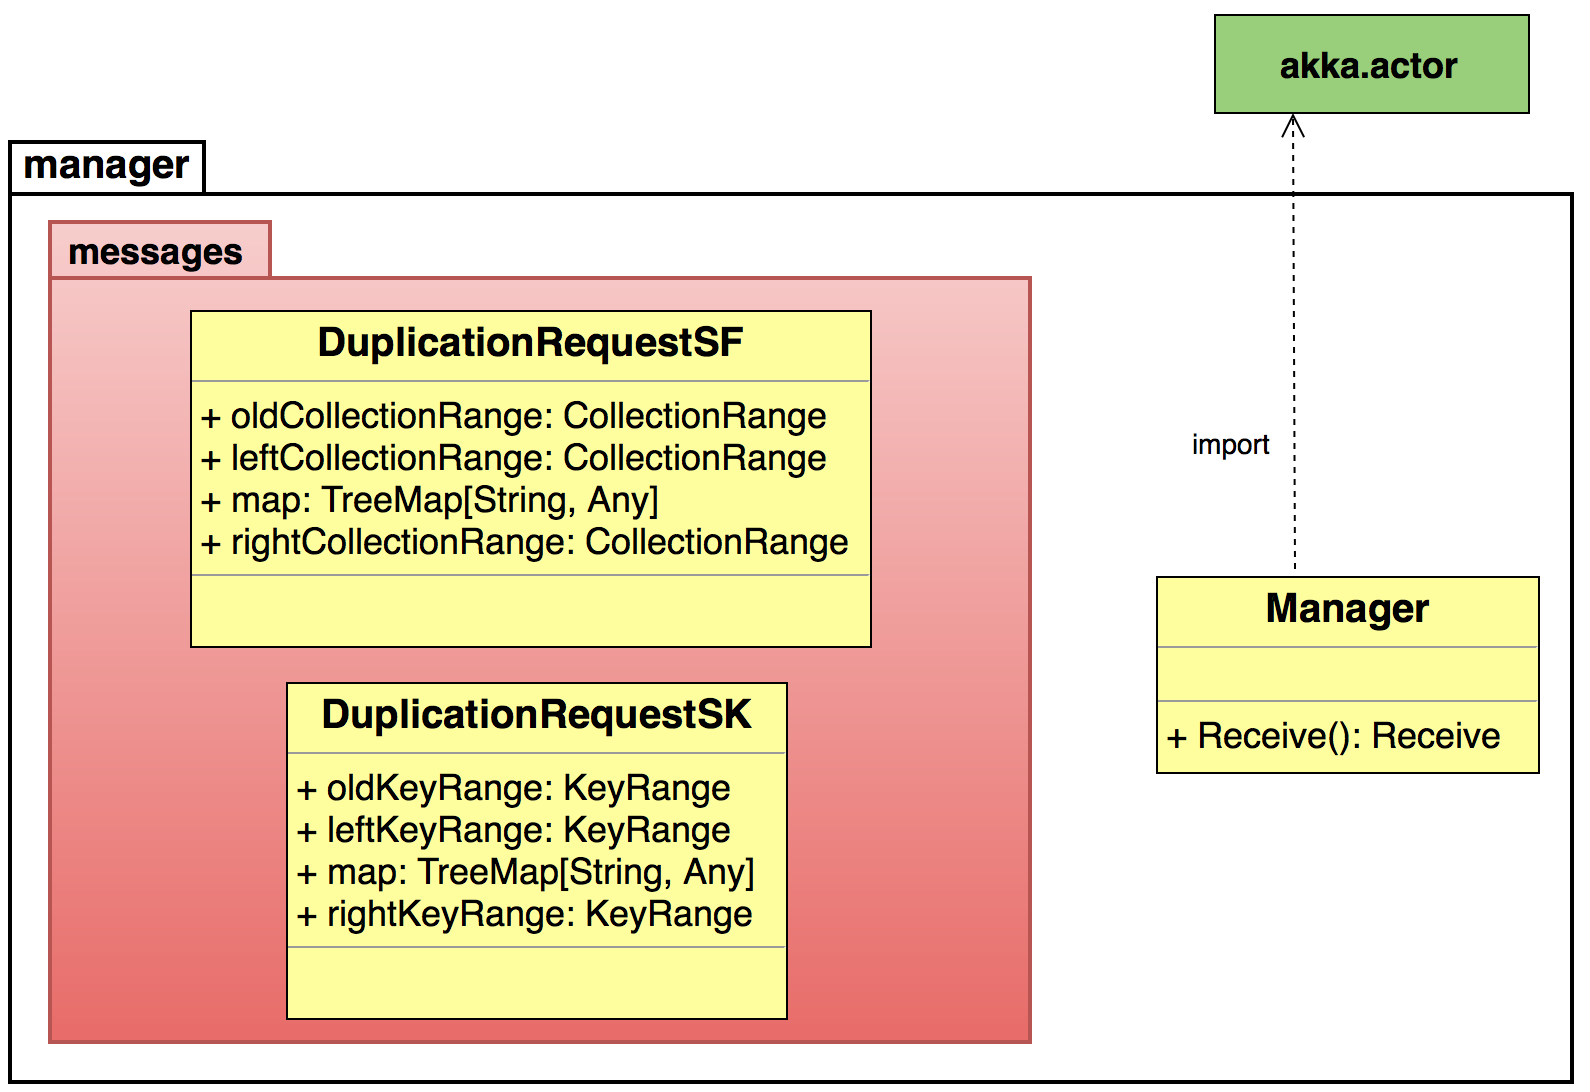
\includegraphics[width=0.8\textwidth,keepaspectratio]{RQ/manager.png}
    \caption{Manager, visione generale del package}
  \end{center}
\end{figure}

\subsubsection{Descrizione}
\gloss{Package} che rappresenta l'\gloss{attore} di tipo \gloss{Manager}.

\subsubsection{Package contenuti}

\begin{itemize}
\item \hyperref[sec:actorbase::actorsystem::manager::messages]{actorbase::actorsystem::manager::messages}.
\end{itemize}

\subsubsection{Interazioni con altre componenti}
\begin{itemize}
\item \hyperref[sec:actorbase::actorsystem::utils]{actorbase::actorsystem::utils}.
\end{itemize}

\subsubsection{Classi}

\paragraph{actorbase::actorsystem::manager::Manager}
\label{sec:actorbase::actorsystem::manager::Manager}

\subparagraph{Descrizione}
Classe che rappresenta un \gloss{attore} di tipo \gloss{Manager}.

\subparagraph{Utilizzo}
Questa classe viene utilizzata per gestire le richieste di divisione di attori di tipo
\hyperref[sec:actorbase::actorsystem::storekeeper::Storekeeper]{Storekeeper}
e \hyperref[sec:actorbase::actorsystem::storefinder::Storefinder]{Storefinder}.

\subparagraph{Classi ereditate}
\begin{itemize}
\item akka::actor::Actor.
\end{itemize}

\subparagraph{Interazioni con altre classi}
\begin{itemize}
\item \hyperref[sec:actorbase::actorsystem::utils::CollectionRange]{actorbase::actorsystem::utils::CollectionRange};
\item \hyperref[sec:actorbase::actorsystem::utils::KeyRange]{actorbase::actorsystem::utils::KeyRange}.
\end{itemize}

\subsection{actorbase::actorsystem::manager::messages}
\label{sec:actorbase::actorsystem::manager::messages}

\begin{figure}[H]
  \begin{center}
    \includegraphics[width=0.6\textwidth,keepaspectratio]{RQ/classiDiag/messages-manager.png}
    \caption{Actorsystem: package messages del manager}
  \end{center}
\end{figure}

\subparagraph{Descrizione}
\gloss{Package} che contiene tutti i messaggi che possono essere ricevuti
dall'\gloss{attore} di tipo
\hyperref[sec:actorbase::actorsystem::manager::Manager]{actorbase::\allowbreak{}actorsystem::\allowbreak{}manager::\allowbreak{}Manager}

\paragraph{actorbase::actorsystem::manager::messages::DuplicationRequestSK}
\label{sec:actorbase::actorsystem::manager::messages::DuplicationRequestSK}

\subparagraph{Descrizione}

Messaggio che richiede la divisione a metà dell'\gloss{attore} di tipo
\hyperref[sec:actorbase::actorsystem::storekeeper::Storekeeper]{Storekeeper}.

\subparagraph{Utilizzo}

Quando \hyperref[sec:actorbase::actorsystem::manager::Manager]{Manager}
riceve questo messaggio provvederà a dividere a metà l'\gloss{attore} di tipo
\hyperref[sec:actorbase::actorsystem::storekeeper::Storekeeper]{Storekeeper}
che dovrà essere diviso.\\Manderà inoltre un messaggio \hyperref[sec:actorbase::actorsystem::storefinder::messages::DuplicateSKNotify]{DuplicateSKNotify} all'\gloss{attore} di tipo
\hyperref[sec:actorbase::actorsystem::storefinder::Storefinder]{Storefinder}
per aggiornare i suoi riferimenti.

\subparagraph{Interazioni con altre classi}
\begin{itemize}
\item \hyperref[sec:actorbase::actorsystem::utils::CollectionRange]{actorbase::actorsystem::utils::CollectionRange};
\item \hyperref[sec:actorbase::actorsystem::utils::KeyRange]{actorbase::actorsystem::utils::KeyRange}.
\end{itemize}

\paragraph{actorbase::actorsystem::manager::messages::DuplicationRequestSF}
\label{sec:actorbase::actorsystem::manager::messages::DuplicationRequestSF}

\subparagraph{Descrizione}

Messaggio che richiede la divisione a metà dell'\gloss{attore} di tipo
\gloss{Storefinder}.

\subparagraph{Utilizzo}

Quando \hyperref[sec:actorbase::actorsystem::manager::Manager]{actorbase::\allowbreak{}actorsystem::\allowbreak{}manager::\allowbreak{}Manager}
riceve questo messaggio provvederà a dividere a metà l'\gloss{attore} di tipo
\hyperref[sec:actorbase::actorsystem::storefinder::Storefinder]{actorbase::\allowbreak{}actorsystem::\allowbreak{}storefinder::\allowbreak{}Storefinder}
che dovrà essere diviso. Manderà inoltre un messaggio all'\gloss{attore} di tipo
\hyperref[sec:actorbase::actorsystem::main::Main]{actorbase::\allowbreak{}actorsystem::\allowbreak{}main::\allowbreak{}Main}
per aggiornare i suoi riferimenti.

\subparagraph{Interazioni con altre classi}
\begin{itemize}
\item \hyperref[sec:actorbase::actorsystem::utils::CollectionRange]{actorbase::actorsystem::utils::CollectionRange};
\item \hyperref[sec:actorbase::actorsystem::utils::KeyRange]{actorbase::actorsystem::utils::KeyRange}.
\end{itemize}

%%%%%%%%%%%%%%%%%%%%%%%%%%%%%%%%%%%%%%%%%%%%%%%%%%%%%%%%%%%%%%%%%%%%
% DRIVER PARTE                              %
%%%%%%%%%%%%%%%%%%%%%%%%%%%%%%%%%%%%%%%%%%%%%%%%%%%%%%%%%%%%%%%%%%%%

\subsection{actorbase::driver}
\label{sec:actorbase::driver}

\begin{figure}[H]
  \begin{center}
    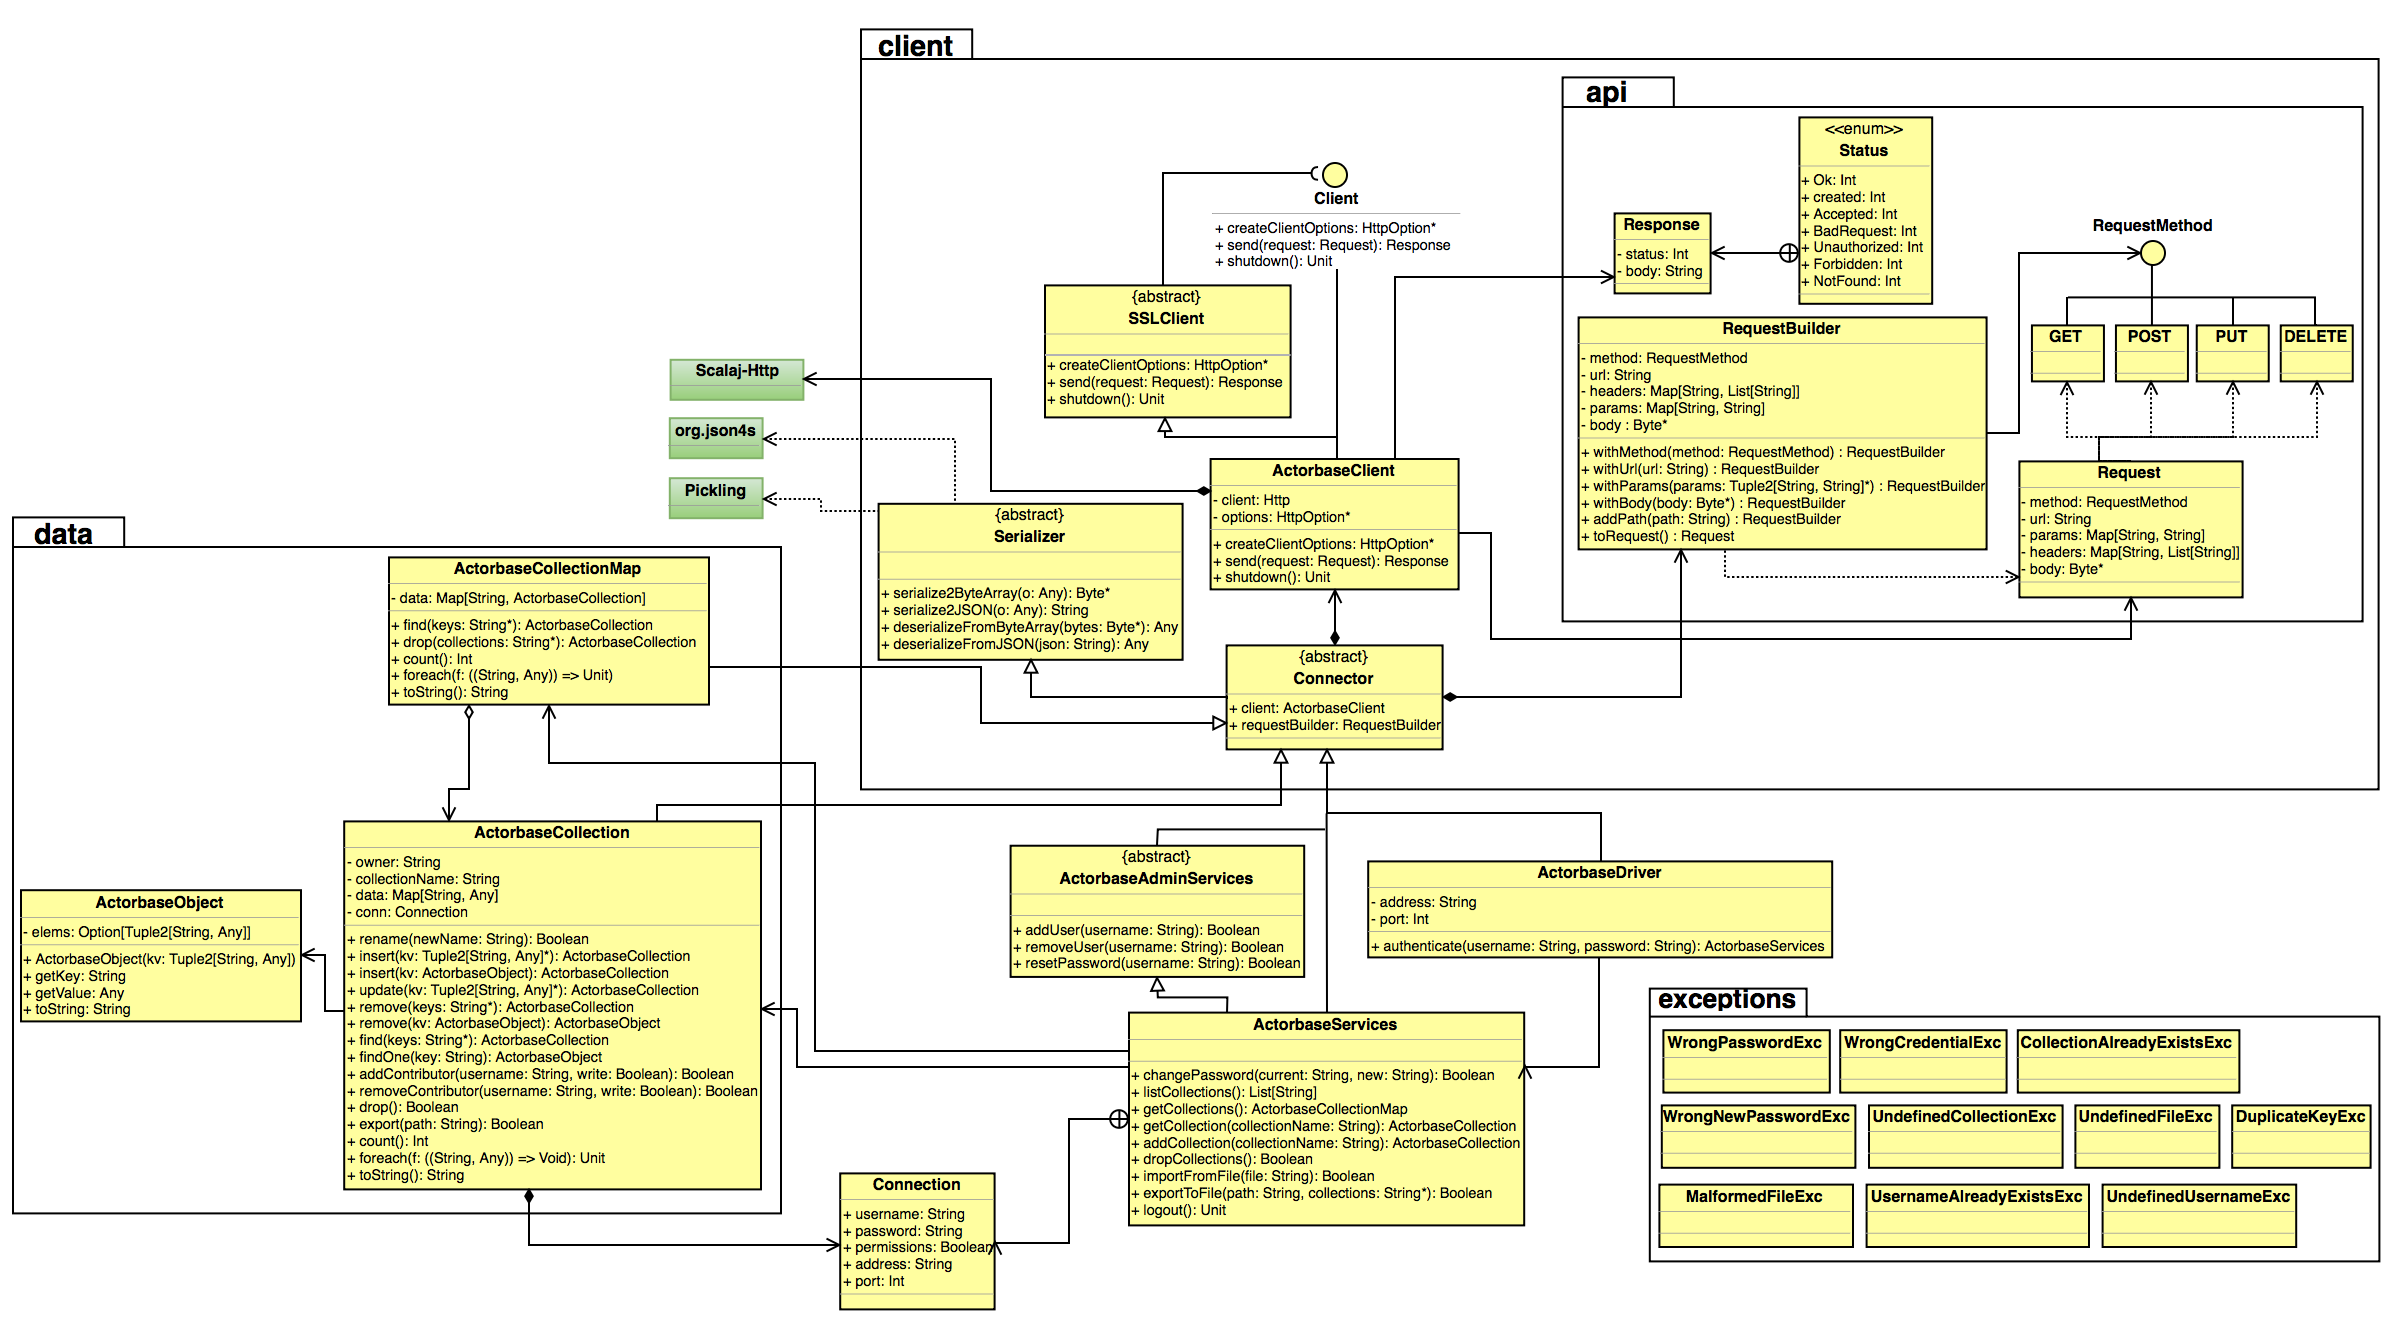
\includegraphics[width=1.0\textwidth,keepaspectratio]{RP/Driver.png}
    \caption{CLI:architettura MVC variante push model}
  \end{center}
\end{figure}

\subsubsection{Descrizione}

\gloss{Package} per la componente \gloss{driver} da utilizzare in un programma
\gloss{Scala}, rappresenta l'interfaccia contenente i metodi designati
all'utilizzo finale in un programma \gloss{Scala}.

\subsubsection{Interazioni con altre componenti}

\begin{itemize}
\item \hyperref[sec:actorbase::cli]{actorbase::cli};
\item \hyperref[sec:actorbase::actorsystem]{actorbase::actorsystem}.
\end{itemize}

\subsubsection{Package contenuti}

\begin{itemize}
\item \hyperref[sec:actorbase::driver::client]{actorbase::driver::client};
\item \hyperref[sec:actorbase::driver::api]{actorbase::driver::api};
\item \hyperref[sec:actorbase::driver::data]{actorbase::driver::data};
\item \hyperref[sec:actorbase::driver::exceptions]{actorbase::driver::exceptions}.
\end{itemize}

\subsubsection{Classi}

\paragraph{ActorbaseDriver}
\label{sec:actorbase::driver::ActorbaseDriver}

\subparagraph{Descrizione}

Classe principale della componente \gloss{driver}, rappresenta l'interfaccia
di connessione e autenticazione con il \gloss{server}.

\subparagraph{Utilizzo}

Espone i metodi di connessione e autenticazione al \gloss{server} \textbf{Actorbase}, e restituisce un oggetto
di tipo \hyperref[sec::actorbase::driver::ActorbaseServices]{ActorbaseServices} in base ai privilegi del proprio
profilo nel sistema.

\subparagraph{Eredita}

\begin{itemize}
\item \hyperref[sec:actorbase::driver::client::Connector]{actorbase::driver::client::Connector}.
\end{itemize}

\subparagraph{Interazioni con le altre classi}

\begin{itemize}
\item \hyperref[sec::actorbase::driver::ActorbaseServices]{actorbase::driver::ActorbaseServices}
\end{itemize}

\paragraph{ActorbaseServices}
\label{sec:actorbase::driver::ActorbaseServices}

\subparagraph{Descrizione}

Classe principale della componente \gloss{driver}, rappresenta l'interfaccia
contenente i metodi designati all'utilizzo di \textbf{Actorbase} in un programma
\gloss{Scala}.

\subparagraph{Utilizzo}

Espone i metodi di interrogazione, ricerca e gestione dei dati
remoti all'interno del \gloss{database}.

\subparagraph{Eredita}

\begin{itemize}
\item \hyperref[sec:actorbase::driver::client::Connector]{actorbase::driver::client::Connector}.
\end{itemize}

\subparagraph{Interazioni con le altre classi}

\begin{itemize}
\item \hyperref[sec:actorbase::driver::client::ActorbaseCollection]{actorbase::driver::client::ActorbaseCollection};
\item \hyperref[sec:actorbase::driver::client::ActorbaseCollection]{actorbase::driver::client::ActorbaseCollectionMap}.
\end{itemize}

\paragraph{ActorbaseAdminServices}
\label{sec:actorbase::driver::ActorbaseAdminServices}

\subparagraph{Descrizione}

Classe principale della componente \gloss{driver}, rappresenta l'interfaccia
contenente i metodi designati all'utilizzo di \textbf{Actorbase} in un programma
\gloss{Scala}.

\subparagraph{Utilizzo}

Aggiunge funzionalità amministrative all'oggetto
\hyperref[sec:actorbase::driver::ActorbaseServices]{ActorbaseServices}, ossia
operazioni di gestione degli utenti.

\subparagraph{Eredita}

\begin{itemize}
\item \hyperref[sec:actorbase::driver::client::ActorbaseServices]{actorbase::driver::client::ActorbaseServices}.
\end{itemize}

\subparagraph{Interazioni con le altre classi}

\begin{itemize}
\item \hyperref[sec:actorbase::driver::client::ActorbaseCollection]{actorbase::driver::client::ActorbaseCollection};
\item \hyperref[sec:actorbase::driver::client::ActorbaseCollection]{actorbase::driver::client::ActorbaseCollectionMap}.
\end{itemize}

\paragraph{Connection}
\label{sec:actorbase::driver::Connection}

\subparagraph{Descrizione}

Classe interna all'oggetto
\hyperref[sec:actorbase::driver::ActorbaseServices]{ActorbaseServices} contenente i
parametri di connessione al \gloss{server} e le credenziali del profilo \textbf{Actorbase}.

\subparagraph{Utilizzo}

Viene utilizzata come oggetto contenente i parametri di connessione, da
utilizzare nelle classi che necessitano di collegamenti al \gloss{server}.

\subparagraph{Interazioni con le altre classi}

\begin{itemize}
\item \hyperref[sec:actorbase::driver::client::data::ActorbaseCollection]{actorbase::driver::client::data::ActorbaseCollection}.
\end{itemize}

\subsection{actorbase::driver::client}
\label{sec:actorbase::driver::client}

\begin{figure}[H]
  \begin{center}
    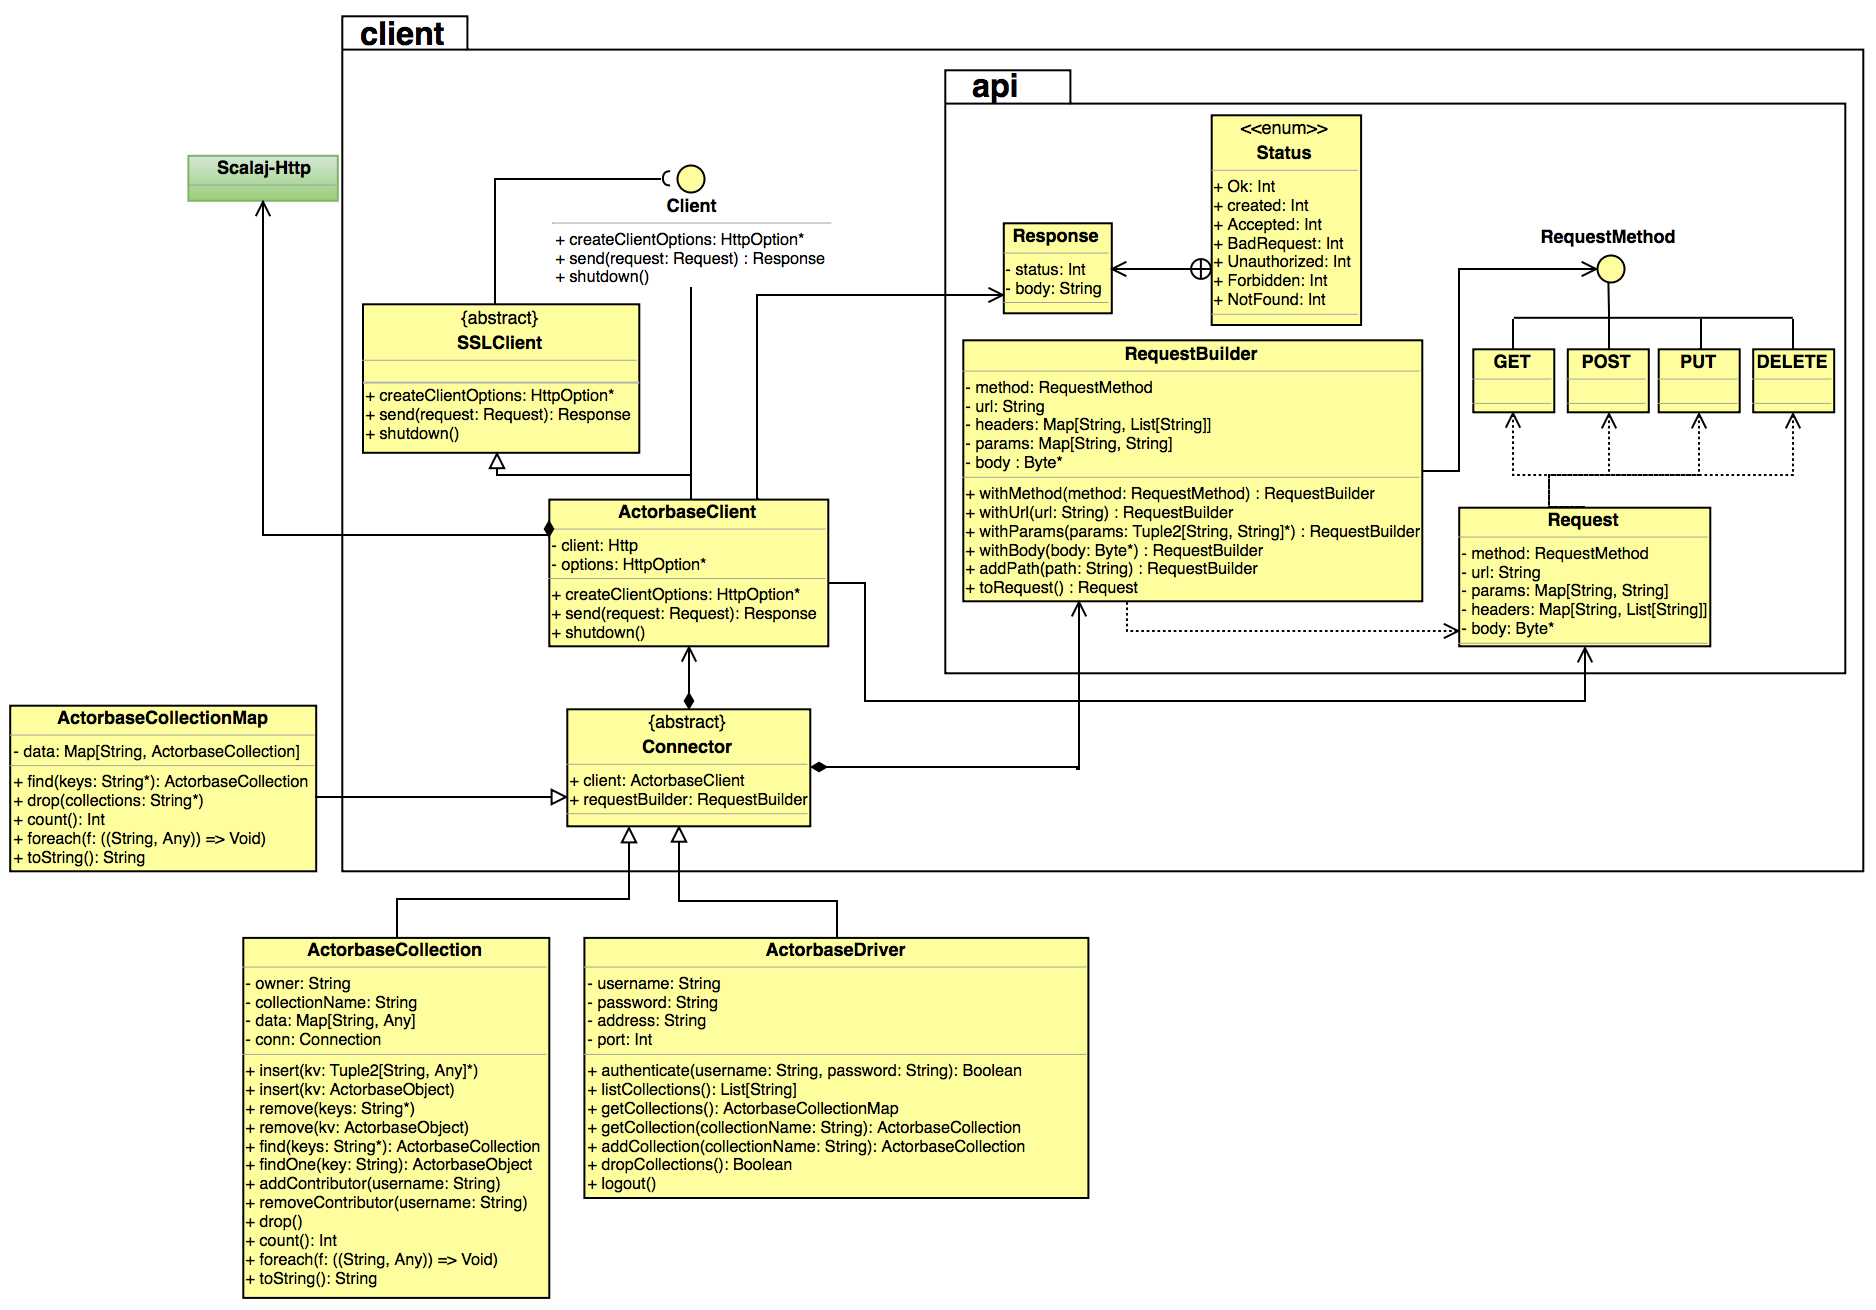
\includegraphics[width=0.9\textwidth,keepaspectratio]{RQ/Client.png}
    \caption{Driver: Packager client}
  \end{center}
\end{figure}

\subsubsection{Descrizione}

\gloss{Package} che si occupa di comunicare sia con la componente \gloss{cli}
che con la componente \gloss{server} del sistema.

\subsubsection{Interazioni con altre componenti}

\begin{itemize}
\item \hyperref[sec:actorbase::cli::models]{actorbase::cli::models};
\item \hyperref[sec:actorbase::actorsystem::clientactor]{actorbase::actorsystem::clientactor}.
\end{itemize}

\subsubsection{Classi}

\paragraph{Client}
\label{sec:actorbase::driver::client::Client}

\subparagraph{Descrizione}

Interfaccia che rappresenta il comportamento di un client atto alla connessione
con un server.

\subparagraph{Utilizzo}

Viene utilizzata per delineare il comportamento generale di un generico client,
le classi che la realizzano hanno libertà di implementazione specifica dei
metodi.

\paragraph{SSLClient (abstract)}
\label{sec:actorbase::driver::client::SSLClient}

\subparagraph{Descrizione}

Classe astratta che rappresenta il comportamento di un client atto alla connessione
protetta con un server.

\subparagraph{Utilizzo}

Viene utilizzata per delineare il comportamento generale di un generico client,
funge da \gloss{Decorator} in quanto aggiunge funzionalità di protezione della
connesione mediante protocolli \gloss{TLS/SSL}, le classi che la realizzano
hanno libertà di implementazione specifica dei metodi.

\subparagraph{Realizza}

\begin{itemize}
\item \hyperref[sec:actorbase::driver::client::Client]{actorbase::driver::client::Client}.
\end{itemize}

\paragraph{actorbase::driver::client::ActorbaseClient}
\label{sec:actorbase::driver::client::ActorbaseClient}

\subparagraph{Descrizione}

Classe che rappresenta il client utilizzato per la connessione con la componente
\gloss{server} del sistema.

\subparagraph{Utilizzo}

Viene utilizzata dalla componente
\hyperref[sec:actorbase::driver::client::Connector]{Connector} per fornire la
comunicazione con la componente \gloss{server} del sistema alle classi che lo
necessitano.

\subparagraph{Realizza}

\begin{itemize}
\item \hyperref[sec:actorbase::driver::client::Client]{actorbase::driver::client::Client}.
\end{itemize}

\subparagraph{Eredita}

\begin{itemize}
\item \hyperref[sec:actorbase::driver::client::SSLClient]{actorbase::driver::client::SSLClient}.
\end{itemize}

\paragraph{Serializer (abstract)}
\label{sec:actorbase::driver::client::Serializer}

\subparagraph{Descrizione}

Classe astratta atta a fornire metodi di serializzazione e deserializzazione nelle
varianti \gloss{JSON} e \gloss{array} di \gloss{byte}.

\subparagraph{Utilizzo}

Viene utilizzata mediante estensione dalle classi che necessitano di operazioni di
serializzazione e deserializzazione in formato \gloss{JSON} o \gloss{array} di byte
o entrambi.

\subparagraph{Ereditata da}

\begin{itemize}
\item \hyperref[sec:actorbase::driver::client::Connector]{actorbase::driver::client::Connector}
\end{itemize}

\paragraph{actorbase::driver::client::Connector (abstract)}
\label{sec:actorbase::driver::client::Connector}

\subparagraph{Descrizione}

Classe astratta che si occupa di istanziare un oggetto di tipo
\hyperref[sec:actorbase::driver::client::ActorbaseClient]{ActorbaseClient} e uno
di tipo
\hyperref[sec:actorbase::driver::client::api::RequestBuilder]{RequestBuilder} in
modo da fornire possibilità di comunicazione con il server alle classi che la
estendono.

\subparagraph{Utilizzo}

Viene estesa dalle classi che necessitano di comunicare con il server.

\subparagraph{Eredita}

\begin{itemize}
\item \hyperref[sec:actorbase::driver::client::Serializer]{actorbase::driver::client::Serializer}
\end{itemize}

\subsection{actorbase::driver::client::api}
\label{sec:actorbase::driver::client::api}

\begin{figure}[H]
  \begin{center}
    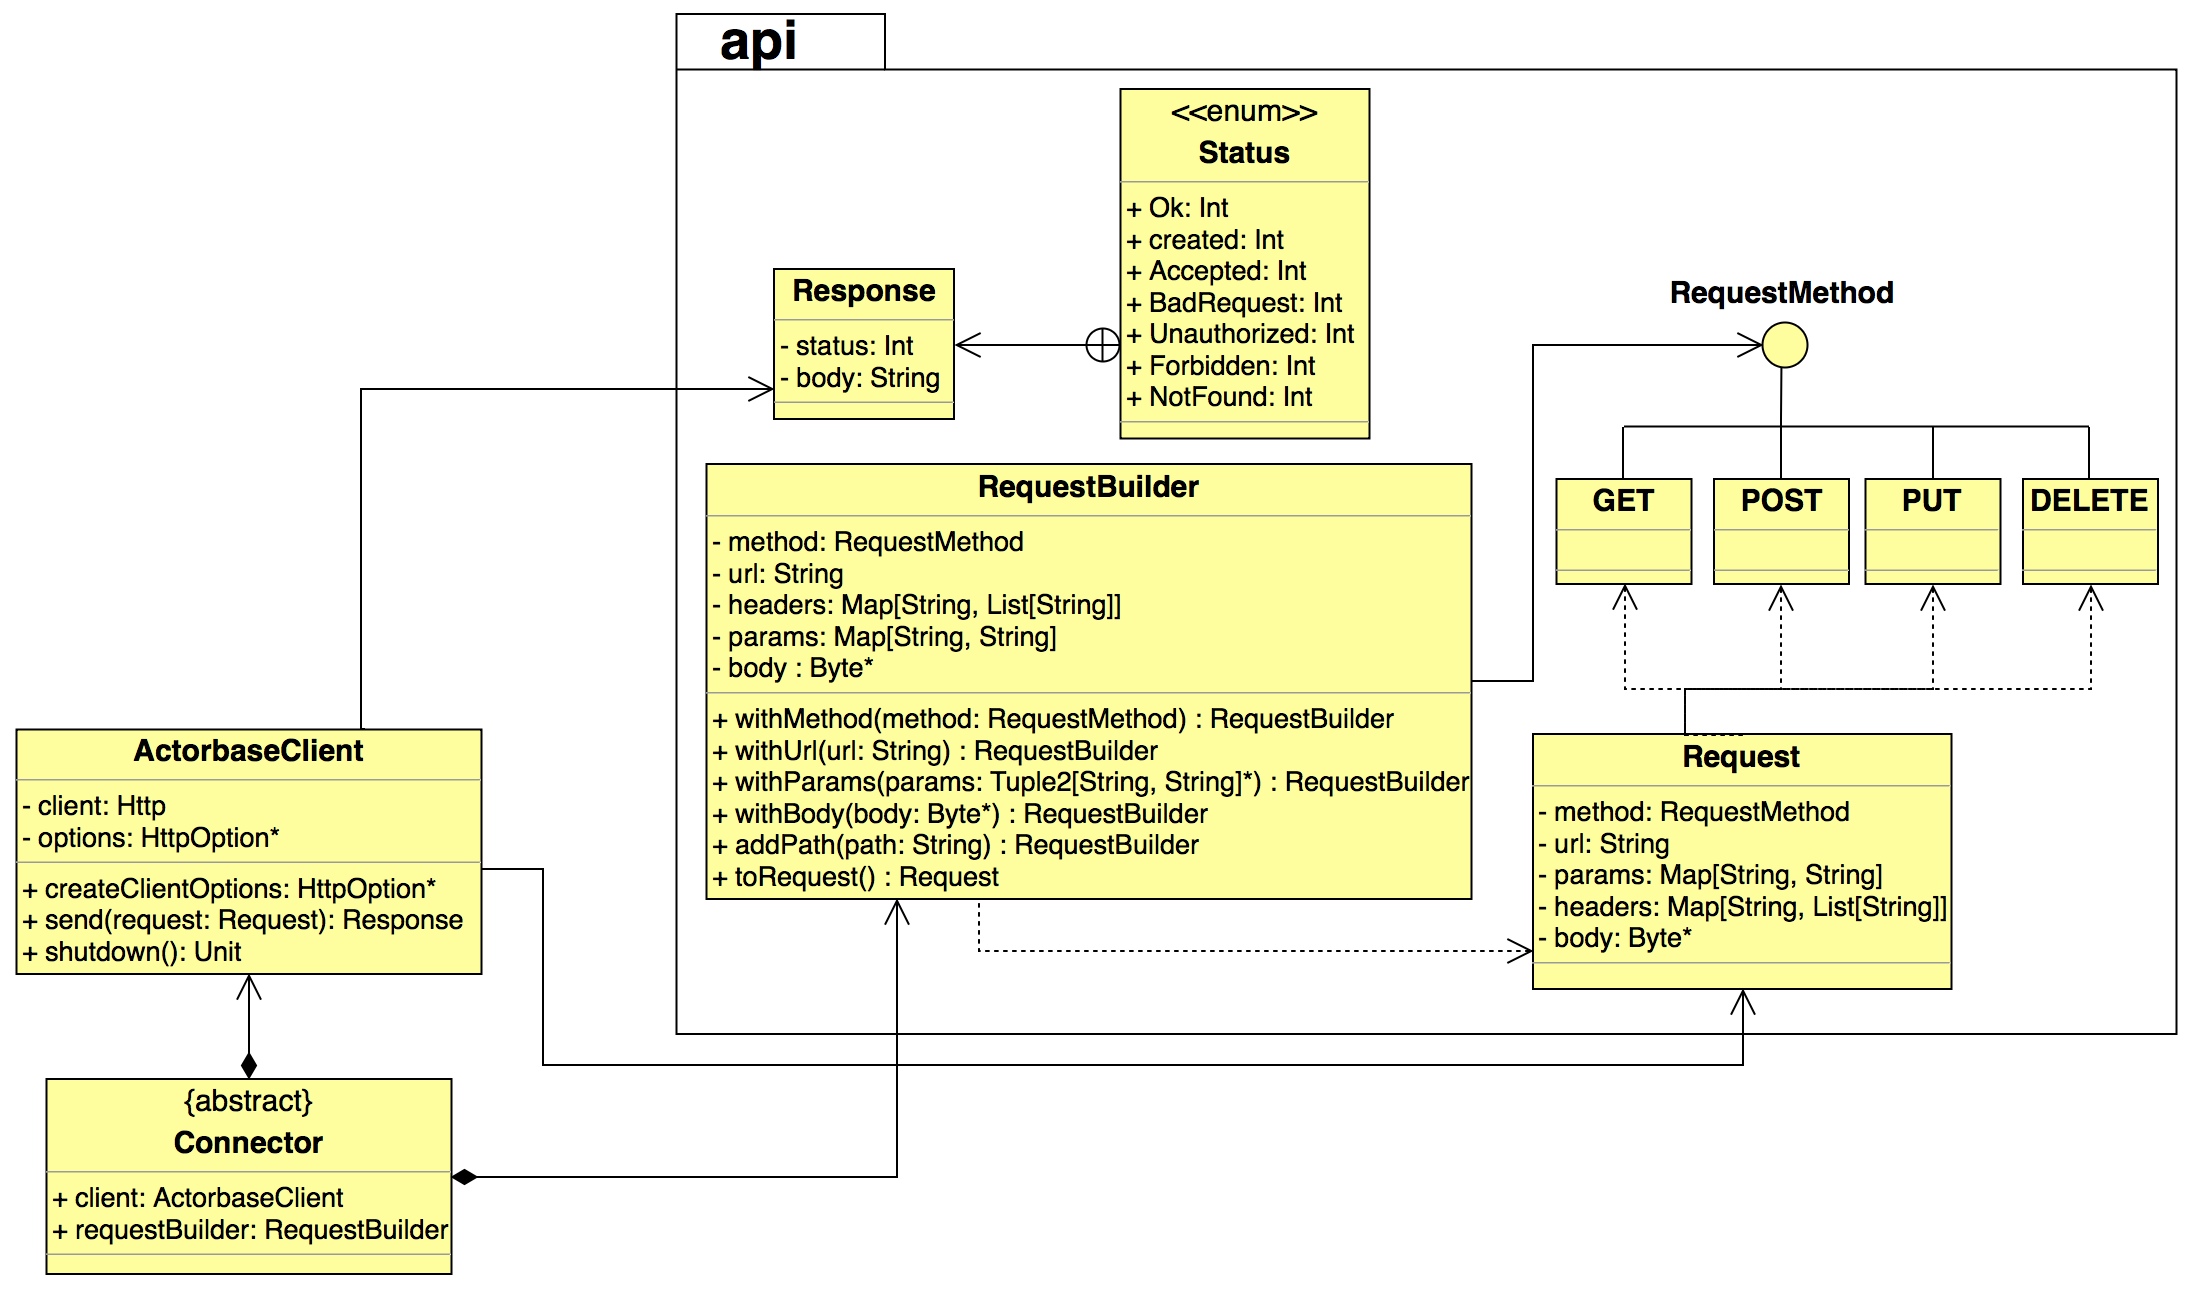
\includegraphics[width=0.9\textwidth,keepaspectratio]{RQ/Api.png}
    \caption{Driver: Package api e interazioni con package client}
  \end{center}
\end{figure}

\subsubsection{Descrizione}

\gloss{Package} che offre le strutture dati necessarie per la comunicazione con
il \gloss{server}, con la \gloss{cli} o eventuali programmi esterni. Si occupa
inoltre della gestione delle richieste \gloss{REST} da inviare utilizzando il
protocollo \gloss{HTTP}.

\subsubsection{Interazioni con altre componenti}
\begin{itemize}
\item \hyperref[sec:actorbase::driver::client]{actorbase::driver::client};
\end{itemize}

\subsubsection{Classi}

\paragraph{actorbase::driver::client::api::RequestMethod (abstract)}
\label{sec:actorbase::driver::client::api::RequestMethod}

\subparagraph{Descrizione}

Classe astratta che rappresenta una generica richiesta \gloss{HTTP},
implementata utilizzando la specifica funzionalità \textit{case class} di Scala,
in modo da poter usufruirne mediante costrutti e algoritmi di \gloss{pattern
  matching}.

\subparagraph{Utilizzo}

Viene utilizzata come classe padre per l'implementazione delle richieste
\gloss{HTTP} da utilizzare nella comunicazione con il server.

\subparagraph{Interazioni con le altre classi}

\begin{itemize}
\item \hyperref[sec:actorbase::driver::client::api::RequestBuilder]{actorbase::driver::client::api::RequestBuilder}.
\end{itemize}

% FINE REQUESTMETHOD

\paragraph{actorbase::driver::client::api::GET (abstract)}
\label{sec:actorbase::driver::client::api::GET}

\subparagraph{Descrizione}

Classe astratta che rappresenta una generica richiesta \gloss{HTTP} di tipo
\gloss{GET}, implementata utilizzando la specifica funzionalità \textit{case
  class} di Scala, in modo da poter usufruirne mediante costrutti e algoritmi di
\gloss{pattern matching}.

\subparagraph{Utilizzo}

Viene utilizzata come classe per l'implementazione delle richieste \gloss{HTTP}
di tipo \gloss{GET} da utilizzare nella comunicazione con il server.

\subparagraph{Interazioni con le altre classi}

\begin{itemize}
\item \hyperref[sec:actorbase::driver::client::api::Request]{actorbase::driver::client::api::Request}.
\end{itemize}

\subparagraph{Eredita}

\begin{itemize}
\item \hyperref[sec:actorbase::driver::client::api::RequestMethod]{actorbase::driver::client::api::RequestMethod}
\end{itemize}

% FINE GET

\paragraph{actorbase::driver::client::api::POST (abstract)}
\label{sec:actorbase::driver::client::api::POST}

\subparagraph{Descrizione}

Classe astratta che rappresenta una generica richiesta \gloss{HTTP} di tipo
\gloss{POST}, implementata utilizzando la specifica funzionalità \textit{case
  class} di Scala, in modo da poter usufruirne mediante costrutti e algoritmi di
\gloss{pattern matching}.

\subparagraph{Utilizzo}

Viene utilizzata come classe per l'implementazione delle richieste \gloss{HTTP}
di tipo \gloss{POST} da utilizzare nella comunicazione con il server.

\subparagraph{Interazioni con le altre classi}

\begin{itemize}
\item \hyperref[sec:actorbase::driver::client::api::Request]{actorbase::driver::client::api::Request}.
\end{itemize}

\subparagraph{Eredita}

\begin{itemize}
\item \hyperref[sec:actorbase::driver::client::api::RequestMethod]{actorbase::driver::client::api::RequestMethod}
\end{itemize}

% FINE POST

\paragraph{actorbase::driver::client::api::PUT (abstract)}
\label{sec:actorbase::driver::client::api::PUT}

\subparagraph{Descrizione}

Classe astratta che rappresenta una generica richiesta \gloss{HTTP} di tipo
\gloss{PUT}, implementata utilizzando la specifica funzionalità \textit{case
  class} di Scala, in modo da poter usufruirne mediante costrutti e algoritmi di
\gloss{pattern matching}.

\subparagraph{Utilizzo}

Viene utilizzata come classe per l'implementazione delle richieste \gloss{HTTP}
di tipo \gloss{PUT} da utilizzare nella comunicazione con il server.

\subparagraph{Interazioni con le altre classi}

\begin{itemize}
\item \hyperref[sec:actorbase::driver::client::api::Request]{actorbase::driver::client::api::Request}.
\end{itemize}

\subparagraph{Eredita}

\begin{itemize}
\item \hyperref[sec:actorbase::driver::client::api::RequestMethod]{actorbase::driver::client::api::RequestMethod}
\end{itemize}

% FINE PUT

\paragraph{actorbase::driver::client::api::DELETE (abstract)}
\label{sec:actorbase::driver::client::api::DELETE}

\subparagraph{Descrizione}

Classe astratta che rappresenta una generica richiesta \gloss{HTTP} di tipo
\gloss{DELETE}, implementata utilizzando la specifica funzionalità \textit{case
  class} di Scala, in modo da poter usufruirne mediante costrutti e algoritmi di
\gloss{pattern matching}.

\subparagraph{Utilizzo}

Viene utilizzata come classe per l'implementazione delle richieste \gloss{HTTP}
di tipo \gloss{DELETE} da utilizzare nella comunicazione con il server.

\subparagraph{Interazioni con le altre classi}

\begin{itemize}
\item \hyperref[sec:actorbase::driver::client::api::Request]{actorbase::driver::client::api::Request}.
\end{itemize}

\subparagraph{Eredita}

\begin{itemize}
\item \hyperref[sec:actorbase::driver::client::api::RequestMethod]{actorbase::driver::client::api::RequestMethod}
\end{itemize}

% FINE DELETE

\paragraph{actorbase::driver::client::api::Request}
\label{sec:actorbase::driver::client::api::Request}

\subparagraph{Descrizione}

Classe che rappresenta una generica richiesta \gloss{HTTP}, implementata
utilizzando la specifica funzionalità \textit{case class} di Scala, in modo da
poter usufruirne mediante costrutti e algoritmi di \gloss{pattern matching},
racchiude al suo interno i parametri di richiesta, quali il metodo, di tipo
\hyperref[sec:actorbase::driver::client::api::RequestMethod]{RequestMethod},
l'\gloss{URL} a cui inviare la richiesta, gli \gloss{header} \gloss{HTTP}
associati, i parametri e il \gloss{payload}.

\subparagraph{Utilizzo}

Viene utilizzata come classe per l'implementazione delle richieste \gloss{HTTP}
di tipo \gloss{DELETE} da utilizzare nella comunicazione con il server. Viene
creata mediante il design pattern \gloss{Builder} nella classe
\hyperref[sec:actorbase::driver::client::api::RequestBuilder]{RequestBuilder}.

\subparagraph{Interazioni con le altre classi}

\begin{itemize}
\item \hyperref[sec:actorbase::driver::client::api::RequestBuilder]{actorbase::driver::client::api::RequestBuilder}.
\item \hyperref[sec:actorbase::driver::client::ActorbaseClient]{actorbase::driver::client::ActorbaseClient}.
\end{itemize}

\paragraph{actorbase::driver::client::api::Response}
\label{sec:actorbase::driver::client::api::Response}

\subparagraph{Descrizione}

Classe che rappresenta una generica risposta \gloss{HTTP}, implementata
utilizzando la specifica funzionalità \textit{case class} di Scala, in modo da
poter usufruirne mediante costrutti e algoritmi di \gloss{pattern matching},
racchiude al suo interno i parametri di risposta, quali il codice di stato,
rappresentato da una enum interna
\hyperref[sec:actorbase::driver::client::api::Status]{Status} e il
\gloss{payload} di risposta in formato stringa.

\subparagraph{Utilizzo}

Viene utilizzata come classe per l'incapsulamento delle risposte \gloss{HTTP} da
utilizzare nella comunicazione con il server.

\subparagraph{Interazioni con le altre classi}

\begin{itemize}
\item \hyperref[sec:actorbase::driver::client::api::Status]{actorbase::driver::client::api::Status};
\item \hyperref[sec:actorbase::driver::client::ActorbaseClient]{actorbase::driver::client::ActorbaseClient}.
\end{itemize}

% FINE RESPONSE

\paragraph{Status}
\label{sec:actorbase::driver::client::api::Status}

\subparagraph{Descrizione}

Enum interna a hyperref[sec:actorbase::driver::client::api::Response]{Response},
rappresenta il codice di ritorno della richiesta \gloss{HTTP} inviata al server.

\subparagraph{Utilizzo}

Viene utilizzata come classe per l'incapsulamento dei codici di ritorno
\gloss{HTTP} da utilizzare nella comunicazione con il server.

\subparagraph{Interazioni con le altre classi}

\begin{itemize}
\item \hyperref[sec:actorbase::driver::client::api::Response]{actorbase::driver::client::api::Response}.
\end{itemize}

% FINE STATUS

\paragraph{RequestBuilder}
\label{sec:actorbase::driver::client::api::RequestBuilder}

\subparagraph{Descrizione}

Rappresenta una classe builder per la creazione di richieste \gloss{HTTP},
racchiude al suo interno i parametri di richiesta, quali il metodo, di tipo
\hyperref[sec:actorbase::driver::client::api::RequestMethod]{RequestMethod},
l'\gloss{URL} a cui inviare la richiesta, gli \gloss{header} \gloss{HTTP}
associati, i parametri e il \gloss{payload} e i metodi \verb=with= per
aggiungere attributi alla richiesta di tipo
\hyperref[sec:actorbase::driver::client::api::Request]{Request} da generare.

\subparagraph{Utilizzo}

Viene utilizzata come classe buider per la costruzione delle richieste
\gloss{HTTP} di tipo
\hyperref[sec:actorbase::driver::client::api::Request]{Request} da utilizzare
nella comunicazione con il server.

\subparagraph{Interazioni con le altre classi}

\begin{itemize}
\item \hyperref[sec:actorbase::driver::client::api::Request]{actorbase::driver::client::api::Request};
\item \hyperref[sec:actorbase::driver::client::Connector]{actorbase::driver::client::Connector}.
\end{itemize}

% FINE API
% SONO QUI 04/05 6:07 P.M.

\subsection{actorbase::driver::client::api::data}
\label{sec:actorbase::driver::client::api::data}

\begin{figure}[H]
  \begin{center}
    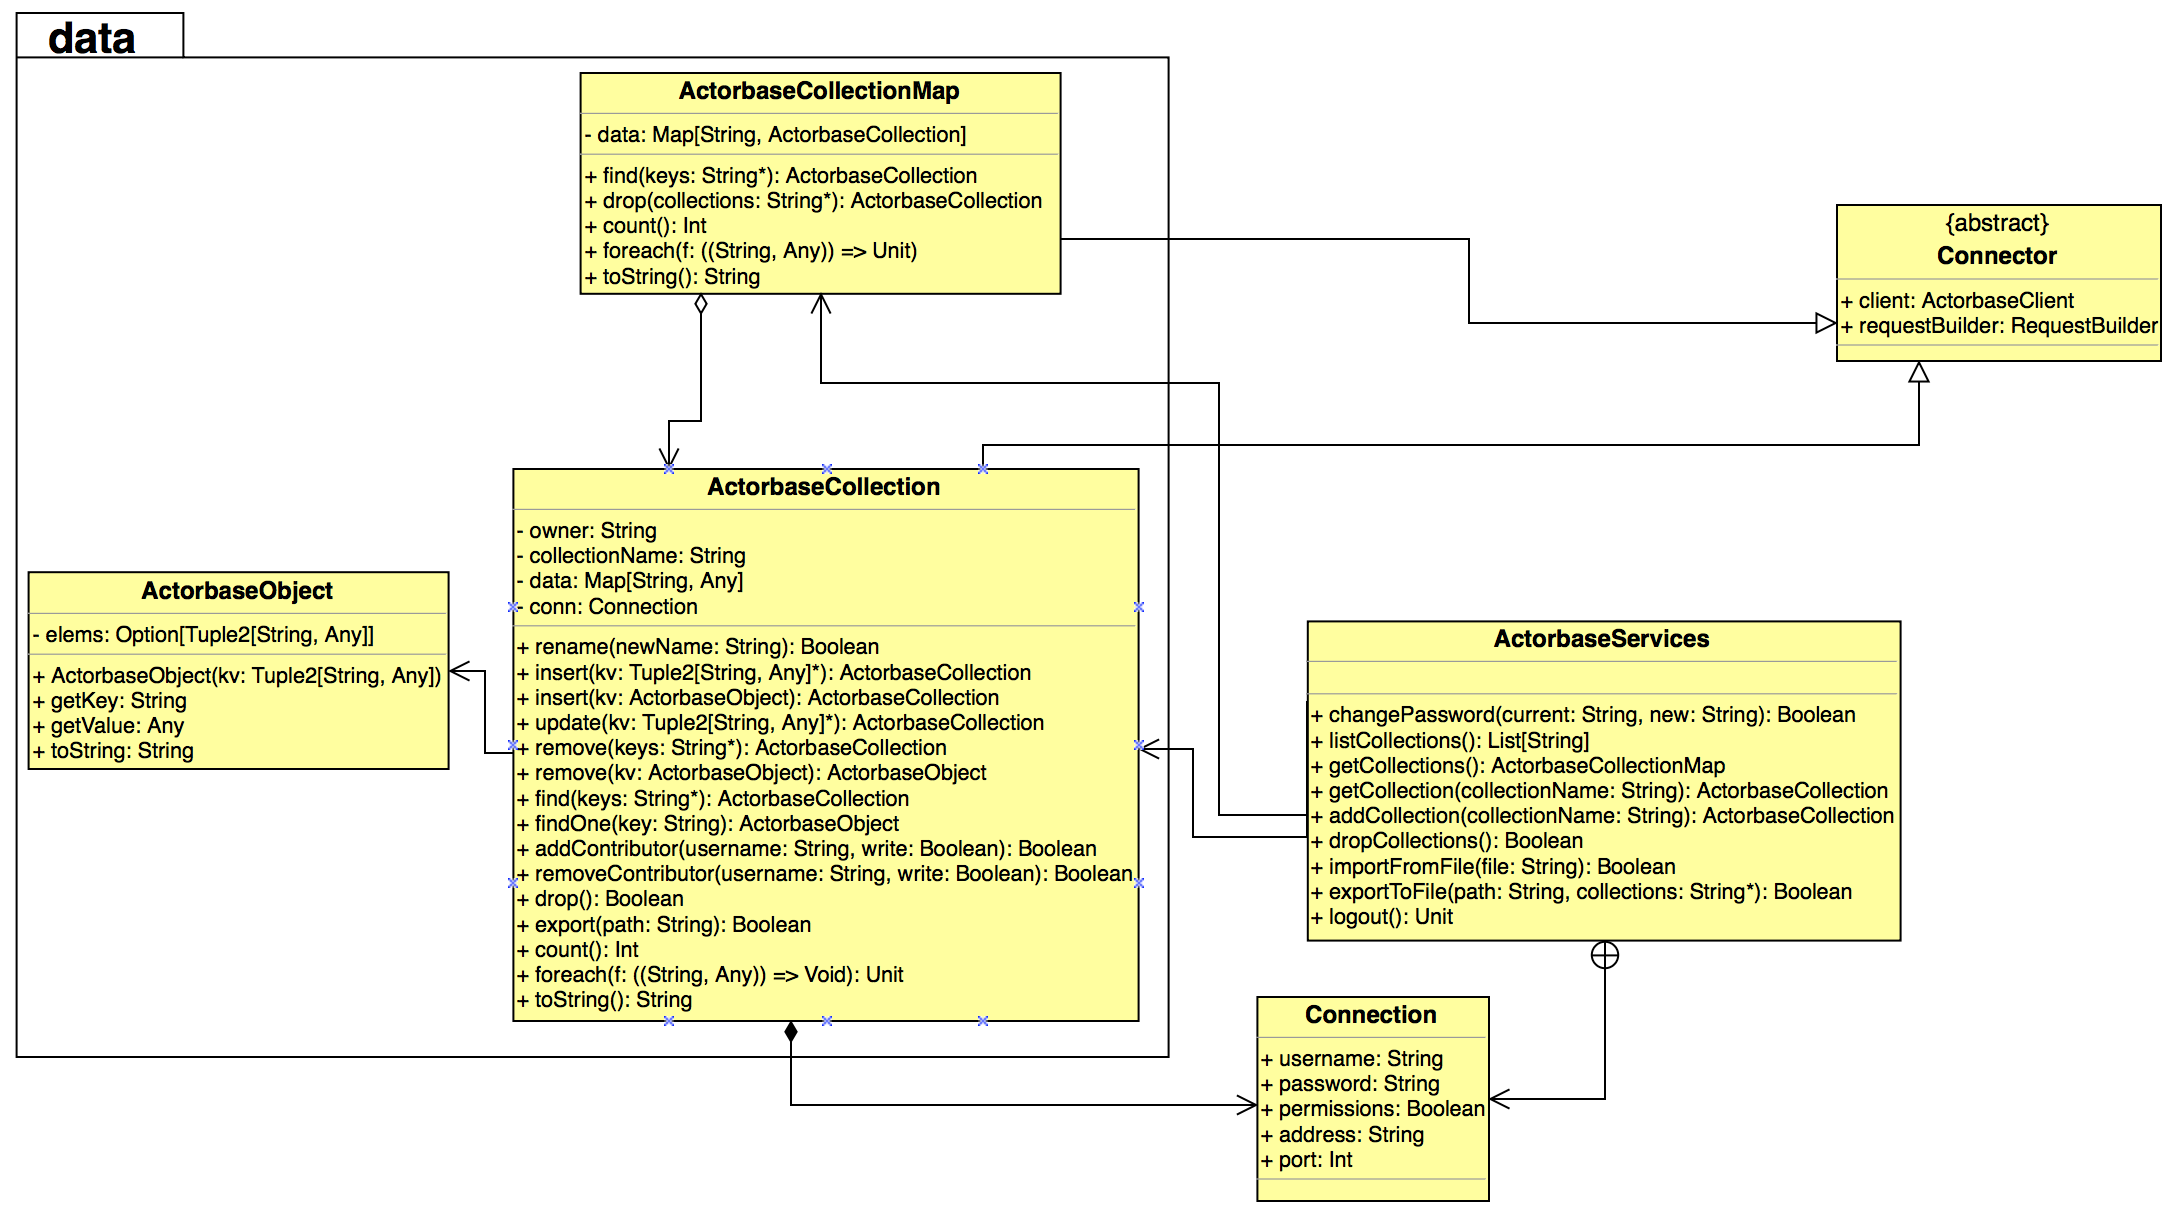
\includegraphics[width=0.9\textwidth,keepaspectratio]{RQ/Data.png}
    \caption{Driver: Package data e interazioni con package padre}
  \end{center}
\end{figure}

\subsubsection{Descrizione}

\gloss{Package} che offre le strutture dati utili alla gestione dei contenuti
della base di dati in locale, permettendo di eseguire le comuni operazioni di
\gloss{CRUD} e ricerche più accurate in maniera semplificata, riflettendo le
eventuali modifiche locali sul server remoto che contiene i dati originali.

\subsubsection{Interazioni con altre componenti}
\begin{itemize}
\item \hyperref[sec:actorbase::driver::client]{actorbase::driver::client}.
\end{itemize}

\subsubsection{Classi}

\paragraph{ActorbaseObject}
\label{sec:actorbase::driver::data::ActorbaseObject}

\subparagraph{Descrizione}

Interfaccia che rappresenta un oggetto generico contenente una coppia
chiave-valore ricevuto dal \gloss{server}.

\subparagraph{Utilizzo}

Classe utilizzata per agevolare le ricerche specifiche all'interno delle
\gloss{collezioni} del \gloss{database}.

\subparagraph{Interazioni con le altre classi}

\begin{itemize}
\item \hyperref[sec:actorbase::driver::client::data::ActorbaseCollection]{actorbase::driver::client::data::ActorbaseCollection}.
\end{itemize}

\paragraph{actorbase::driver::data::ActorbaseCollection}
\label{sec:actorbase::driver::data::ActorbaseCollection}

\subparagraph{Descrizione}

Classe che rappresenta una singola \gloss{collezione} del \gloss{database}.

\subparagraph{Utilizzo}

Questa classe viene utilizzata per la rappresentazione di una singola
\gloss{collezione} vista come insieme di oggetti di tipo coppia chiave-valore.
Il valore può essere qualsiasi tipo, inclusi oggetti arbitrari creati
all'interno di un programma \gloss{Scala}. Offre metodi di utilità e
navigabilità dei contenuti.

\subparagraph{Eredita}

\begin{itemize}
\item \hyperref[sec:actorbase::driver::data::Serializer]{actorbase::driver::data::Serializer}.
\end{itemize}

\subparagraph{Interazioni con le altre classi}

\begin{itemize}
\item \hyperref[sec:actorbase::driver::client::data::ActorbaseObject]{actorbase::driver::client::data::ActorbaseObject}.
\item \hyperref[sec:actorbase::driver::client::data::ActorbaseCollectionMap]{actorbase::driver::client::data::ActorbaseCollectionMap}.
\end{itemize}

\paragraph{actorbase::driver::data::ActorbaseCollectionMap}
\label{sec:actorbase::driver::data::ActorbaseCollectionMap}

\subparagraph{Descrizione}

Classe che rappresenta una \gloss{collezione} di \gloss{collezione} del sistema.

\subparagraph{Utilizzo}

Questa classe viene utilizzata per la rappresentazione dell'aggregazione di
\gloss{collezioni}, è formata da una mappa di coppie nomecollezione -
\hyperref[sec:actorbase::driver::data::ActorbaseCollection]{ActorbaseCollection}.

\subparagraph{Eredita}

\begin{itemize}
\item \hyperref[sec:actorbase::driver::data::Serializer]{actorbase::driver::data::Serializer}.
\end{itemize}

\subparagraph{Interazioni con le altre classi}

\begin{itemize}
\item \hyperref[sec:actorbase::driver::client::ActorbaseDriver]{actorbase::driver::client::ActorbaseDriver}.
\item \hyperref[sec:actorbase::driver::client::data::ActorbaseCollection]{actorbase::driver::client::data::ActorbaseCollection}.
\end{itemize}

% FINE DATA

\subsection{actorbase::driver::exceptions}
\label{sec:actorbase::driver::exceptions}

\begin{figure}[H]
  \begin{center}
    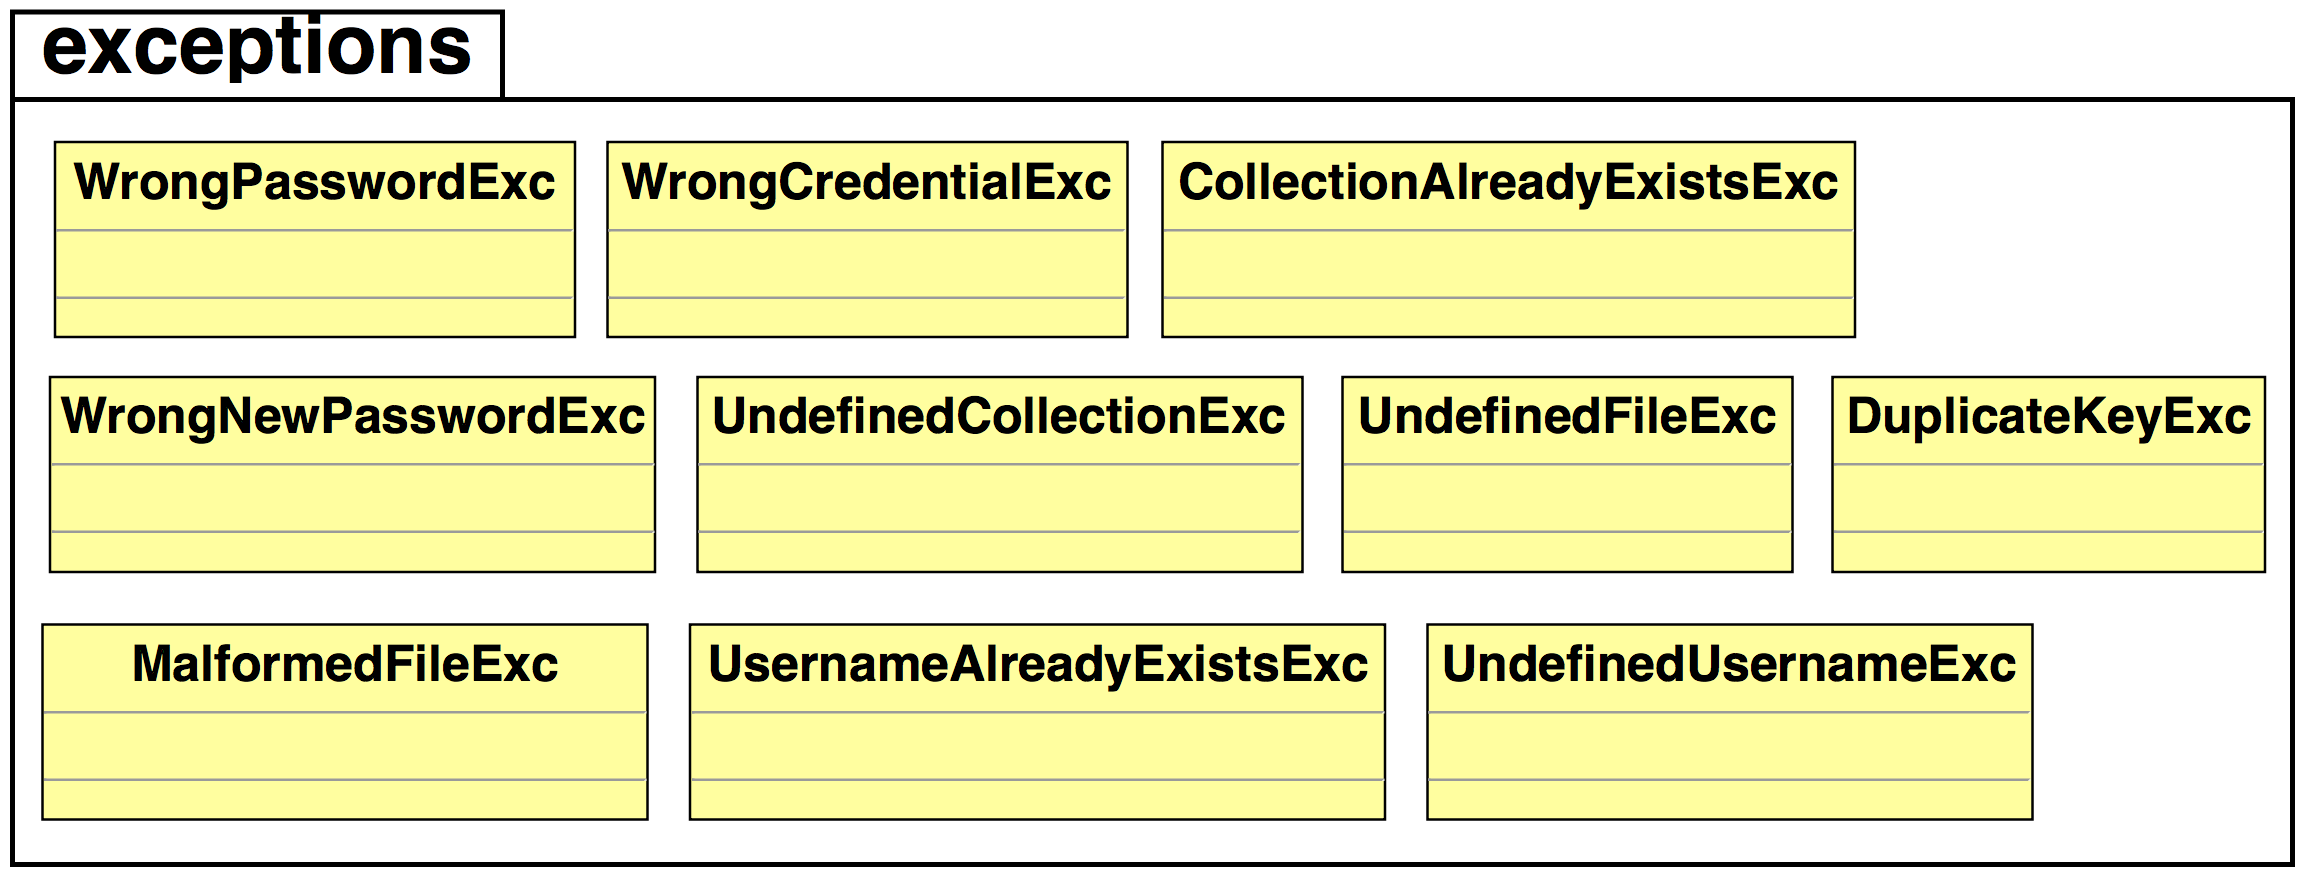
\includegraphics[width=0.7\textwidth,keepaspectratio]{RQ/Exceptions.png}
    \caption{Driver: Package exceptions}
  \end{center}
\end{figure}

\subsubsection{Descrizione}

\gloss{Package} che contiene le possibili eccezioni che si possono verificare nel \gloss{driver}

\subsubsection{Interazione con altre componenti}
\begin{itemize}
\item \hyperref[sec:actorbase::driver::client]{actorbase::driver::client};
\end{itemize}

\subsubsection{Classi}

\paragraph{actorbase::driver::exceptions::WrongCredentialExc}

\subparagraph{Descrizione}

Classe che rappresenta l'eccezione del tentativo di accesso con username o password sbagliati.

\subparagraph{Utilizzo}

Questa classe viene utilizzata dal \gloss{driver} per gestire errori nelle credenziali di accesso.

\subparagraph{Interazioni con altre classi}

\begin{itemize}
\item \hyperref[sec:actorbase::driver::client::ActorbaseClient]{actorbase::driver::client::ActorbaseClient}.
\end{itemize}

\paragraph{actorbase::driver::exceptions::WrongPasswordExc}

\subparagraph{Descrizione}

Classe che rappresenta l'eccezione dell'inserimento sbagliato della vecchia password.

\subparagraph{Utilizzo}

Questa classe viene utilizzata dal \gloss{driver} per gestire il caso in cui alla modifica della propria password, quando dovrei inserire la vecchia password questa non corrisponda.

\subparagraph{Interazioni con altre classi}

\begin{itemize}
\item \hyperref[sec:actorbase::driver::client::ActorbaseClient]{actorbase::driver::client::ActorbaseClient}.
\end{itemize}

\paragraph{actorbase::driver::exceptions::WrongNewPasswordExc}

\subparagraph{Descrizione}

Classe che rappresenta l'eccezione dell'inserimento sbagliato della nuova password.

\subparagraph{Utilizzo}

Questa classe viene utilizzata dal \gloss{driver} per gestire il caso in cui alla modifica della propria password, quando dovrei inserire la nuova password questa non soddisfi i requisiti richiesti.

\subparagraph{Interazioni con altre classi}

\begin{itemize}
\item \hyperref[sec:actorbase::driver::client::ActorbaseClient]{actorbase::driver::client::ActorbaseClient}.
\end{itemize}

\paragraph{actorbase::driver::exceptions::CollectionAlreadyExistsExc}

\subparagraph{Descrizione}

Classe che rappresenta l'eccezione del conflitto di nomi tra una collezione esistente e una nuova.

\subparagraph{Utilizzo}

Questa classe viene utilizzata dal \gloss{driver} per gestire il caso in cui alla creazione di una nuova collezione, il nome della nuova collezione corrisponda al nome di una collezione già esistente.

\subparagraph{Interazioni con altre classi}

\begin{itemize}
\item \hyperref[sec:actorbase::driver::client::ActorbaseClient]{actorbase::driver::client::ActorbaseClient}.
\end{itemize}

\paragraph{actorbase::driver::exceptions::UndefinedCollectionExc}

\subparagraph{Descrizione}

Classe che rappresenta l'eccezione di mancato inserimento del nome di una nuova collezione.

\subparagraph{Utilizzo}

Questa classe viene utilizzata dal \gloss{driver} per gestire il caso in cui alla creazione di una nuova collezione, venga omesso il nome di quest'ultima.

\subparagraph{Interazioni con altre classi}

\begin{itemize}
\item \hyperref[sec:actorbase::driver::client::ActorbaseClient]{actorbase::driver::client::ActorbaseClient}.
\end{itemize}

\paragraph{actorbase::driver::exceptions::UndefinedUsernameExc}

\subparagraph{Descrizione}

Classe che rappresenta l'eccezione di mancato inserimento dell'username utente.

\subparagraph{Utilizzo}

Questa classe viene utilizzata dal \gloss{driver} per gestire il caso in cui alla registrazione di un nuovo utente, venga omesso l'username.

\subparagraph{Interazioni con altre classi}

\begin{itemize}
\item \hyperref[sec:actorbase::driver::client::ActorbaseClient]{actorbase::driver::client::ActorbaseClient}.
\end{itemize}

\paragraph{actorbase::driver::exceptions::UsernameAlreadyExistsExc}

\subparagraph{Descrizione}

Classe che rappresenta l'eccezione del conflitto di username tra un utente già esistente e uno nuovo.

\subparagraph{Utilizzo}

Questa classe viene utilizzata dal \gloss{driver} per gestire il caso in cui alla registrazione di un nuovo utente, l'username di quest'ultimo corrisponda all'username di un utente già esistente.

\subparagraph{Interazioni con altre classi}

\begin{itemize}
\item \hyperref[sec:actorbase::driver::client::ActorbaseClient]{actorbase::driver::client::ActorbaseClient}.
\end{itemize}

\paragraph{actorbase::driver::exceptions::DuplicateKeyExc}

\subparagraph{Descrizione}

Classe che rappresenta l'eccezione del conflitto tra una chiave già esistente e una nuova chiave.

\subparagraph{Utilizzo}

Questa classe viene utilizzata dal \gloss{driver} per gestire il caso in cui all'inserimento di una nuova chiave, questa corrisponda ad una chiave già esistente nella stessa collezione.

\subparagraph{Interazioni con altre classi}

\begin{itemize}
\item \hyperref[sec:actorbase::driver::client::ActorbaseClient]{actorbase::driver::client::ActorbaseClient}.
\end{itemize}

\paragraph{actorbase::driver::exceptions::UndefinedFileExc}

\subparagraph{Descrizione}

Classe che rappresenta l'eccezione di inserimento di un path sbagliato di un file o del mancato inserimento del path.

\subparagraph{Utilizzo}

Questa classe viene utilizzata dal \gloss{driver} per gestire il caso in cui all'inserimento di un nuovo item o di una serie di item da file, si sbagli il path del file o si ometta di inserirlo.

\subparagraph{Interazioni con altre classi}

\begin{itemize}
\item \hyperref[sec:actorbase::driver::client::ActorbaseClient]{actorbase::driver::client::ActorbaseClient}.
\end{itemize}

\paragraph{actorbase::driver::exceptions::MalformedFileExc}

\subparagraph{Descrizione}

Classe che rappresenta l'eccezione di inserimento di un path di un file non conforme.

\subparagraph{Utilizzo}

Questa classe viene utilizzata dal \gloss{driver} per gestire il caso in cui all'inserimento di un nuovo item o di una serie di item da file, si inserisca il path di un file in un formato sbagliato o il cui testo non rispetta le regole di formattazione.

\subparagraph{Interazioni con altre classi}

\begin{itemize}
\item \hyperref[sec:actorbase::driver::client::ActorbaseClient]{actorbase::driver::client::ActorbaseClient}.
\end{itemize}

%%%%%%%%%%%%%%%%%%%%%%%%%%%%%%%%%%%%%%%%%%%%%%%%%%%%%%%%%%%%%%%%%%%%
% CLI PARTE                              %
%%%%%%%%%%%%%%%%%%%%%%%%%%%%%%%%%%%%%%%%%%%%%%%%%%%%%%%%%%%%%%%%%%%%

\subsection{actorbase::cli}
\label{sec:actorbase::cli}

\begin{figure}[H]
  \begin{center}
    \includegraphics[width=1.0\textwidth,keepaspectratio]{RQ/CLI.png}
    \caption{CLI, architettura MVC variante push model}
  \end{center}
\end{figure}

\subsubsection{Descrizione}

\gloss{Package} per la parte di \gloss{client} rappresentata dalla \gloss{cli}.
Questa componente viene rappresentata usando il \gloss{design pattern}
\gloss{MVC} in versione \gloss{push model}.

\subsubsection{Interazioni con altre componenti}

\begin{itemize}
\item \hyperref[sec:actorbase::driver]{actorbase::driver}.
\end{itemize}

\subsubsection{Package contenuti}

\begin{itemize}
\item \hyperref[sec:actorbase::cli::views]{actorbase::cli::views};
\item \hyperref[sec:actorbase::cli::controllers]{actorbase::cli::controllers};
\item \hyperref[sec:actorbase::cli::models]{actorbase::cli::models}.
\end{itemize}

\subsection{actorbase::cli::views}
\label{sec:actorbase::cli::views}

\begin{figure}[H]
  \begin{center}
    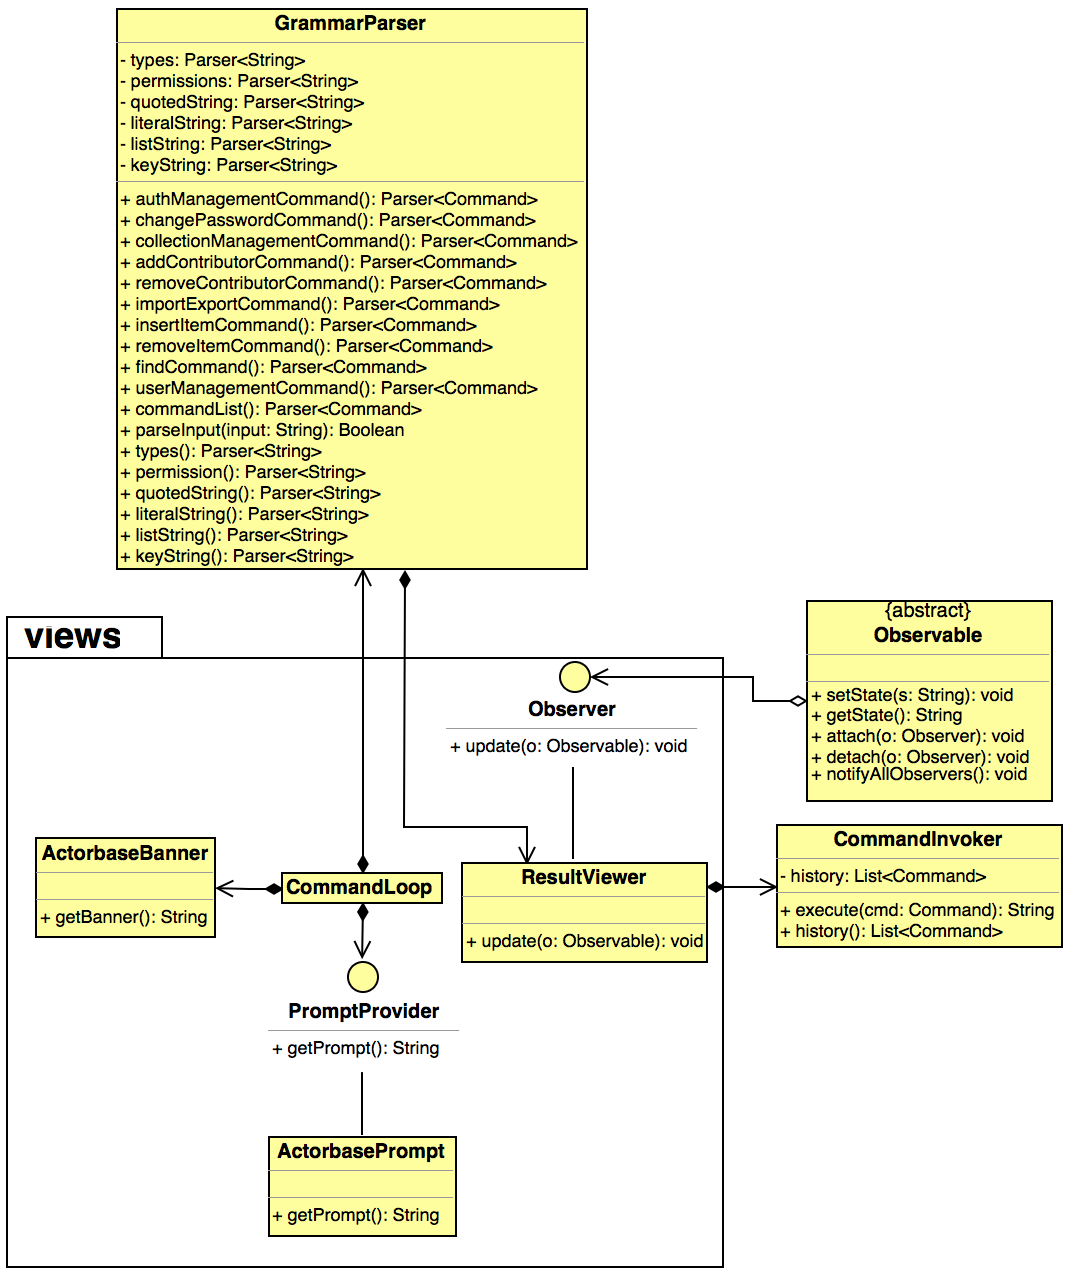
\includegraphics[width=0.8\textwidth,keepaspectratio]{RQ/Views.png}
    \caption{CLI, views package, interazioni con controllers e models}
  \end{center}
\end{figure}

\subsubsection{Descrizione}

\gloss{Package} per la parte \gloss{view} della \gloss{cli}. Questa componente
gestisce l'output e offre l'interfaccia tramite cui l'utente può inserire i
comandi.

\subsubsection{Interazioni con altre componenti}

\begin{itemize}
\item \hyperref[sec:actorbase::cli::controllers]{actorbase::cli::controllers};
\item \hyperref[sec:actorbase::cli::models]{actorbase::cli::models}.
\end{itemize}

\subsubsection{Classi}

\paragraph{actorbase::cli::views::CommandLoop}
\label{sec:actorbase::cli::views::CommandLoop}

\subparagraph{Descrizione}

Questa classe verrà utilizzata per leggere i comandi inseriti dall'utente.

\subparagraph{Utilizzo}

Viene utilizzata per la lettura dei comandi inseriti dall'utente.

\subparagraph{Interazioni con altre classi}

\begin{itemize}
\item \hyperref[sec:actorbase::cli::views::PromptProvider]{actorbase::cli::views::PromptProvider};
\item \hyperref[sec:actorbase::cli::views::ActorbaseBanner]{actorbase::cli::views::ActorbaseBanner};
\item \hyperref[sec:actorbase::cli::views::ResultView]{actorbase::cli::views::ResultView};
\item \hyperref[sec:actorbase::cli::controllers::GrammarParser]{actorbase::cli::controllers::GrammarParser}.
\end{itemize}

\paragraph{actorbase::cli::views::ActorbaseBanner}
\label{sec:actorbase::cli::views::ActorbaseBanner}

\subparagraph{Descrizione}

Classe per la creazione del \gloss{banner} da mostrare all'avvio della
\gloss{CLI}.

\subparagraph{Utilizzo}

Viene utilizzata per la creazione di un \gloss{banner} di presentazione
all'avvio della \gloss{CLI}.

\subparagraph{Interazioni con altre classi}

\begin{itemize}
\item \hyperref[sec:actorbase::cli::views::CommandLoop]{actorbase::cli::views::CommandLoop}.
\end{itemize}

\paragraph{actorbase::cli::views::PromptProvider}
\label{sec:actorbase::cli::views::PromptProvider}

\subparagraph{Descrizione}

Interfaccia per la creazione del \gloss{prompt} dei comandi.

\subparagraph{Utilizzo}

Offre un'interfaccia per la creazione di un \gloss{prompt} generico.

\subparagraph{Interazioni con altre classi}

\begin{itemize}
\item \hyperref[sec:actorbase::cli::views::CommandLoop]{actorbase::cli::views::CommandLoop}.
\end{itemize}

\paragraph{actorbase::cli::views::ActorbasePrompt}
\label{sec:actorbase::cli::views::ActorbasePrompt}

\subparagraph{Descrizione}

Classe che implementa l'interfaccia \hyperref[sec:actorbase::cli::views::PromptProvider]{actorbase::cli::views::PromptProvider} per
la creazione di un \gloss{prompt} dei comandi.

\subparagraph{Utilizzo}

Viene utilizzata per la creazione di un \gloss{prompt} per l'inserimento dei
comandi e la visualizzazione delle informazioni relative alla connessione
effettuata. %TODO: scrivere meglio

\subparagraph{Classi ereditate}

\begin{itemize}
\item \hyperref[sec:actorbase::cli::views::PromptProvider]{actorbase::cli::views::PromptProvider}.
\end{itemize}

\paragraph{actorbase::cli::views::Observer}
\label{sec:actorbase::cli::views::Observer}

\subparagraph{Descrizione}

Interfaccia per l'implementazione del \gloss{design pattern} \gloss{Observer}
che permette di aggiornare la \gloss{view} ad ogni risposta della componente
\gloss{driver}.

\subparagraph{Utilizzo}

Offre un'interfaccia per permettere di aggiornare la \gloss{view} ad ogni
risposta ricevuta dal \gloss{driver}.

\subparagraph{Interazioni con altre classi}

\begin{itemize}
\item \hyperref[sec:actorbase::cli::models::Observable]{actorbase::cli::models::Observable}.
\end{itemize}

\paragraph{actorbase::cli::views::ResultView}
\label{sec:actorbase::cli::views::ResultView}

\subparagraph{Descrizione}

Classe per la gestione e la formattazione in output dei risultati ottenuti
dall'esecuzione del comando ricevuto in input tramite il \gloss{design
  pattern} \gloss{Observer}.

\subparagraph{Utilizzo}

Viene utilizzata per la gestione e la formattazione in output dei risultati
ottenuti dal server mediante l'inserimento dei comandi tramite il
\gloss{design pattern} \gloss{Observer}.

\subparagraph{Classi ereditate}

\begin{itemize}
\item \hyperref[sec:actorbase::cli::views::Observer]{actorbase::cli::views::Observer}.
\end{itemize}

\subparagraph{Interazioni con altre classi}

\begin{itemize}
\item \hyperref[sec:actorbase::cli::views::CommandLoop]{actorbase::cli::views::CommandLoop}.
\end{itemize}

\subsection{actorbase::cli::controllers}
\label{sec:actorbase::cli::controllers}

\begin{figure}[H]
  \begin{center}
    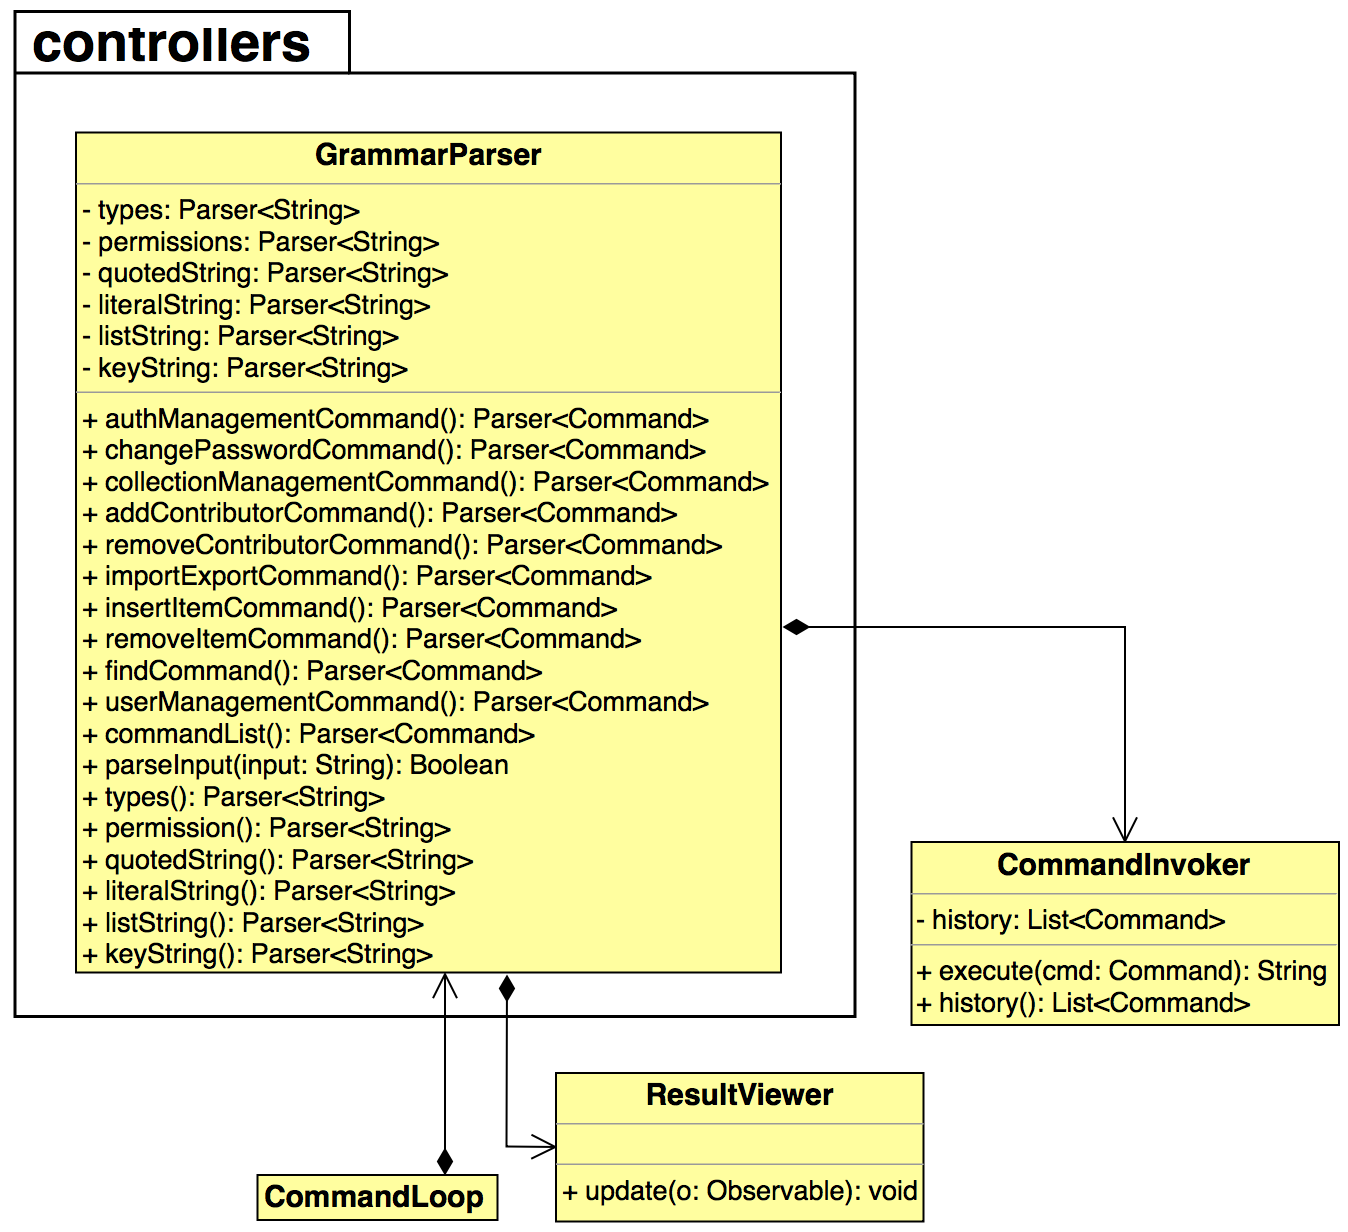
\includegraphics[width=1.0\textwidth,keepaspectratio]{RQ/Controllers.png}
    \caption{CLI: package controllers e interazioni con package models e views}
  \end{center}
\end{figure}

\subsubsection{Descrizione}

\gloss{Package} per la parte \gloss{controller} della \gloss{cli}. Questa
componente si occupa di passare il comando ricevuto dalla \gloss{view} al
\gloss{model}.

\subsubsection{Interazioni con altre componenti}

\begin{itemize}
\item \hyperref[sec:actorbase::cli::views]{actorbase::cli::views};
\item \hyperref[sec:actorbase::cli::models]{actorbase::cli::models}.
\end{itemize}

\subsubsection{Classi}

\paragraph{actorbase::cli::controllers::GrammarParser}
\label{sec:actorbase::cli::controllers::GrammarParser}

\subparagraph{Descrizione}

Classe che si occupa di effettuare il \gloss{parsing} del comando ricevuto
dalla componente \gloss{view} e di chiamare la componente \gloss{model} con i
parametri opportuni.

\subparagraph{Utilizzo}

Viene utilizzata per effettuare il \gloss{parsing} del comando ricevuto da
\hyperref[sec:actorbase::cli::views::CommandLoop]{actorbase::cli::views::CommandLoop} e, in seguito, chiamare
\hyperref[sec:actorbase::cli::models::CommandInvoker]{actorbase::cli::models::CommandInvoker} con i parametri corretti per
l'esecuzione del comando.

\subparagraph{Interazioni con altre classi}

\begin{itemize}
\item \hyperref[sec:actorbase::cli::views::CommandLoop]{actorbase::cli::views::CommandLoop};
\item \hyperref[sec:actorbase::cli::models::CommandInvoker]{actorbase::cli::models::CommandInvoker}.
\end{itemize}

\subsection{actorbase::cli::models}
\label{sec:actorbase::cli::models}

\begin{figure}[H]
  \begin{center}
    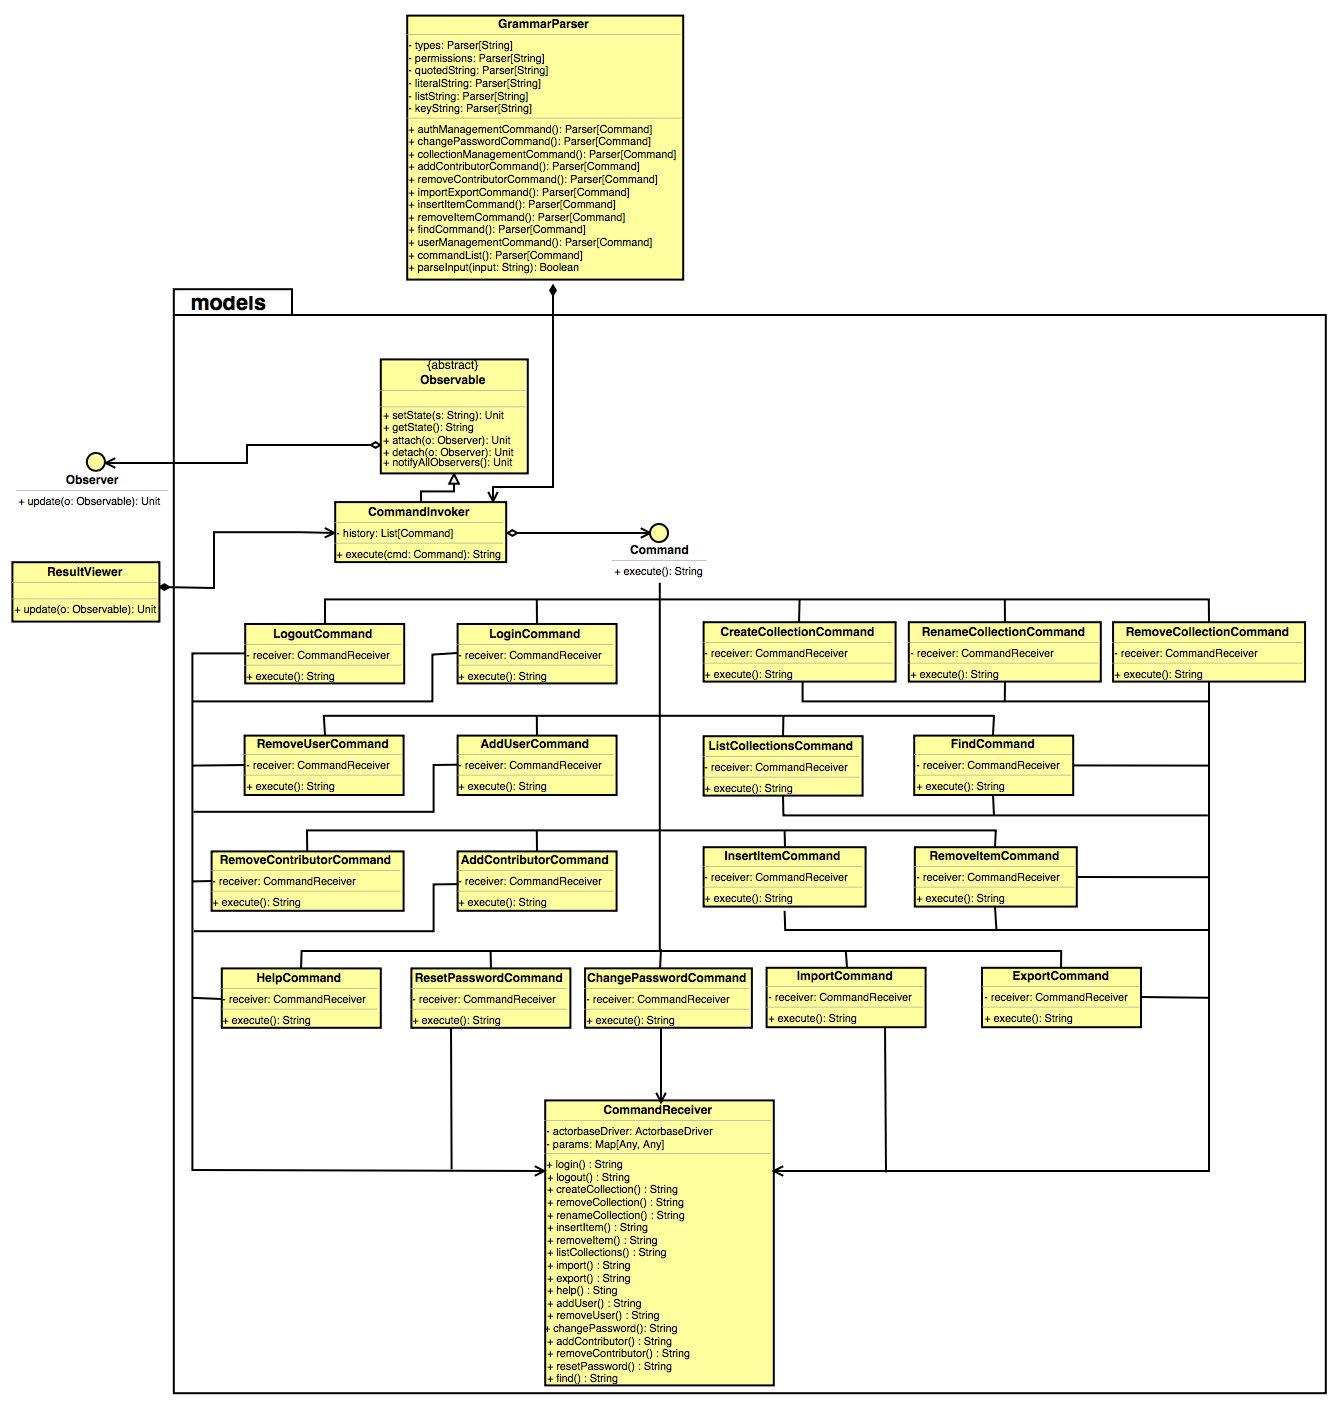
\includegraphics[width=0.8\textwidth,keepaspectratio]{RQ/Models.png}
    \caption{CLI: package models e interazioni con controllers e views}
  \end{center}
\end{figure}

\subsubsection{Descrizione}

\gloss{Package} per la parte \gloss{model} della \gloss{cli}. Questa
componente si occupa della comunicazione con la componente \gloss{driver} e
con la componente \gloss{view} tramite il \gloss{push model} del \gloss{design
  pattern} \gloss{observer}. Per la gestione dei comandi si è scelto di
utilizzare il \gloss{command pattern}.

\subsubsection{Classi}

\paragraph{actorbase::cli::models::Observable}
\label{sec:actorbase::cli::models::Observable}

\subparagraph{Descrizione}

Questa classe rappresenta l'oggetto osservato nell'ambito del \gloss{design
  pattern} \gloss{observer}.

\subparagraph{Utilizzo}

Viene utilizzata per notificare la classe \hyperref[sec:actorbase::cli::views::Observer]{actorbase::cli::views::Observer}
quando avviene una modifica al proprio stato, ossia quando il \gloss{driver}
ha ritornato un risultato.

\subparagraph{Interazioni con altre classi}

\begin{itemize}
\item \hyperref[sec:actorbase::cli::views::Observer]{actorbase::cli::views::Observer}.
\end{itemize}

\paragraph{actorbase::cli::models::CommandInvoker}
\label{sec:actorbase::cli::models::CommandInvoker}

\subparagraph{Descrizione}

Questa classe rappresenta l'\gloss{Invoker} del \gloss{command pattern}. Essa
si occupa di eseguire il comando ricevuto dalla componente \gloss{controller}.

\subparagraph{Utilizzo}

Viene utilizzata per eseguire il comando ricevuto da
\hyperref[sec:actorbase::cli::controllers::GrammarParser]{actorbase::cli::controllers::GrammarParser} chiamando il metodo opportuno che
implementa l'interfaccia \hyperref[sec:actorbase::cli::models::Command]{actorbase::cli::models::Command}.

\subparagraph{Classi ereditate}

\begin{itemize}
\item \hyperref[sec:actorbase::cli::models::Observable]{actorbase::cli::models::Observable}.
\end{itemize}

\subparagraph{Interazioni con altre classi}

\begin{itemize}
\item \hyperref[sec:actorbase::cli::controllers::GrammarParser]{actorbase::cli::controllers::GrammarParser};
\item \hyperref[sec:actorbase::cli::models::Command]{actorbase::cli::models::Command}.
\end{itemize}

\paragraph{actorbase::cli::models::Command}
\label{sec:actorbase::cli::models::Command}

\subparagraph{Descrizione}

Interfaccia generica che rappresenta un comando.

\subparagraph{Utilizzo}

Viene utilizzata per offrire un'interfaccia comune a tutti i comandi.\\Ha un
riferimento a \hyperref[sec:actorbase::cli::models::CommandReceiver]{actorbase::cli::models::CommandReceiver} per l'esecuzione del
comando.

\subparagraph{Interazioni con altre classi}

\begin{itemize}
\item \hyperref[sec:actorbase::cli::models::CommandInvoker]{actorbase::cli::models::CommandInvoker};
\item \hyperref[sec:actorbase::view::cli::models::CommandReceiver]{actorbase::view::cli::models::CommandReceiver}.
\end{itemize}

\paragraph{actorbase::cli::models::FindCommand}
\label{sec:actorbase::cli::models::FindCommand}

\subparagraph{Descrizione}

Classe per il comando di ricerca.

\subparagraph{Utilizzo}

Viene utilizzata per chiamare il metodo di
\hyperref[sec:actorbase::cli::models::CommandReceiver]{actorbase::cli::models::CommandReceiver} per la ricerca con i parametri immessi
dall'utente.

\subparagraph{Classi ereditate}

\begin{itemize}
\item \hyperref[sec:actorbase::cli::models::Command]{actorbase::cli::models::Command}.
\end{itemize}

\paragraph{actorbase::cli::models::LogoutCommand}
\label{sec:actorbase::cli::models::LogoutCommand}

\subparagraph{Descrizione}

Classe per il comando di logout.

\subparagraph{Utilizzo}

Viene utilizzata per chiamare il metodo di
\hyperref[sec:actorbase::cli::models::CommandReceiver]{actorbase::cli::models::CommandReceiver} per il logout.

\subparagraph{Classi ereditate}

\begin{itemize}
\item \hyperref[sec:actorbase::cli::models::Command]{actorbase::cli::models::Command}.
\end{itemize}

\paragraph{actorbase::cli::models::ResetPasswordCommand}
\label{sec:actorbase::cli::models::ResetPasswordCommand}

\subparagraph{Descrizione}

Classe per il comando di reset della password.

\subparagraph{Utilizzo}

Viene utilizzata per chiamare il metodo di
\hyperref[sec:actorbase::cli::models::CommandReceiver]{actorbase::cli::models::CommandReceiver} per il reset della password
dell'utente specificato in input.

\subparagraph{Classi ereditate}

\begin{itemize}
\item \hyperref[sec:actorbase::cli::models::Command]{actorbase::cli::models::Command}.
\end{itemize}

\paragraph{actorbase::cli::models::ChangePasswordCommand}
\label{sec:actorbase::cli::models::ChangePasswordCommand}

\subparagraph{Descrizione}

Classe per il comando di modifica della password.

\subparagraph{Utilizzo}

Viene utilizzata per chiamare il metodo di
\hyperref[sec:actorbase::cli::models::CommandReceiver]{actorbase::cli::models::CommandReceiver} per la modifica della password..

\subparagraph{Classi ereditate}

\begin{itemize}
\item \hyperref[sec:actorbase::cli::models::Command]{actorbase::cli::models::Command}.
\end{itemize}

\paragraph{actorbase::cli::models::ListCommand}
\label{sec:actorbase::cli::models::ListCommand}

\subparagraph{Descrizione}

Classe per il comando di visualizzazione dell'elenco dei nomi di tutte le
collezioni presenti nel \gloss{database}.

\subparagraph{Utilizzo}

Viene utilizzata per chiamare il metodo di
\hyperref[sec:actorbase::cli::models::CommandReceiver]{actorbase::cli::models::CommandReceiver} per la visualizzazione dell'elenco dei
nomi di tutte le collezioni presenti nel \gloss{database}.

\subparagraph{Classi ereditate}

\begin{itemize}
\item \hyperref[sec:actorbase::cli::models::Command]{actorbase::cli::models::Command}.
\end{itemize}

\paragraph{actorbase::cli::models::AddContributorCommand}
\label{sec:actorbase::cli::models::AddContributorCommand}

\subparagraph{Descrizione}

Classe per il comando di aggiunta collaboratore a una collezione.

\subparagraph{Utilizzo}

Viene utilizzata per chiamare il metodo di
\hyperref[sec:actorbase::cli::models::CommandReceiver]{actorbase::cli::models::CommandReceiver} per l'aggiunta di un collaboratore a
una collezione con il nome della \gloss{collezione} e lo username specificati
in input.

\subparagraph{Classi ereditate}

\begin{itemize}
\item \hyperref[sec:actorbase::cli::models::Command]{actorbase::cli::models::Command}.
\end{itemize}

\paragraph{actorbase::cli::models::LoginCommand}
\label{sec:actorbase::cli::models::LoginCommand}

\subparagraph{Descrizione}

Classe per il comando di login.

\subparagraph{Utilizzo}

Viene utilizzata per chiamare il metodo di
\hyperref[sec:actorbase::cli::models::CommandReceiver]{actorbase::cli::models::CommandReceiver} per il login con le credenziali
immesse dall'utente.

\subparagraph{Classi ereditate}

\begin{itemize}
\item \hyperref[sec:actorbase::cli::models::Command]{actorbase::cli::models::Command}.
\end{itemize}

\paragraph{actorbase::cli::models::RemoveCollectionCommand}
\label{sec:actorbase::cli::models::RemoveCollectionCommand}

\subparagraph{Descrizione}

Classe per il comando di rimozione una \gloss{collezione}.

\subparagraph{Utilizzo}

Viene utilizzata per chiamare il metodo di
\hyperref[sec:actorbase::cli::models::CommandReceiver]{actorbase::cli::models::CommandReceiver} per la rimozione di una collezione con
i parametri specificati in input.

\subparagraph{Classi ereditate}

\begin{itemize}
\item \hyperref[sec:actorbase::cli::models::Command]{actorbase::cli::models::Command}.
\end{itemize}

\paragraph{actorbase::cli::models::RemoveContributorCommand}
\label{sec:actorbase::cli::models::RemoveContributorCommand}

\subparagraph{Descrizione}

Classe per il comando di rimozione di un collaboratore da una collezione.

\subparagraph{Utilizzo}

Viene utilizzata per chiamare il metodo di
\hyperref[sec:actorbase::cli::models::CommandReceiver]{actorbase::cli::models::CommandReceiver} per la rimozione di un collaboratore
da una collezione con con il nome della \gloss{collezione} e lo username
specificati in input.

\subparagraph{Classi ereditate}

\begin{itemize}
\item \hyperref[sec:actorbase::cli::models::Command]{actorbase::cli::models::Command}.
\end{itemize}

\paragraph{actorbase::cli::models::RenameCollectionCommand}
\label{sec:actorbase::cli::models::RenameCollectionCommand}

\subparagraph{Descrizione}

Classe per il comando rinominazione di una \gloss{collezione}.

\subparagraph{Utilizzo}

Viene utilizzata per chiamare il metodo di \hyperref[sec:actorbase::cli::models::CommandReceiver]{actorbase::cli::models::CommandReceiver} per la rinominazione di una \gloss{collezione} con i parametri specificati in input.

\subparagraph{Classi ereditate}

\begin{itemize}
\item \hyperref[sec:actorbase::cli::models::Command]{actorbase::cli::models::Command}.
\end{itemize}

\paragraph{actorbase::cli::models::AddUserCommand}
\label{sec:actorbase::cli::models::AddUserCommand}

\subparagraph{Descrizione}

Classe per il comando di aggiunta di un utente.

\subparagraph{Utilizzo}

Viene utilizzata per chiamare il metodo di
\hyperref[sec:actorbase::cli::models::CommandReceiver]{actorbase::cli::models::CommandReceiver} per l'aggiunta di un utente con i
parametri specificati in input.

\subparagraph{Classi ereditate}

\begin{itemize}
\item \hyperref[sec:actorbase::cli::models::Command]{actorbase::cli::models::Command}.
\end{itemize}

\paragraph{actorbase::cli::models::HelpCommand}
\label{sec:actorbase::cli::models::HelpCommand}

\subparagraph{Descrizione}

Classe per la richiesta di aiuto.

\subparagraph{Utilizzo}

Viene utilizzata per chiamare il metodo di
actorbase::cli::models::CommandReceiver per la richiesta di aiuto con i
parametri immessi dall'utente.

\paragraph{actorbase::cli::models::RemoveItemCommand}
\label{sec:actorbase::cli::models::RemoveItemCommand}

\subparagraph{Descrizione}

Classe per il comando di rimozione di un \gloss{item}.

\subparagraph{Utilizzo}

Viene utilizzata per chiamare il metodo di
\hyperref[sec:actorbase::cli::models::CommandReceiver]{actorbase::cli::models::CommandReceiver} per la rimozione di un \gloss{item}
con i parametri immessi dall'utente.

\subparagraph{Classi ereditate}

\begin{itemize}
\item \hyperref[sec:actorbase::cli::models::Command]{actorbase::cli::models::Command}.
\end{itemize}

\paragraph{actorbase::cli::models::RemoveUserCommand}
\label{sec:actorbase::cli::models::RemoveUserCommand}

\subparagraph{Descrizione}

Classe per il comando di rimozione di un utente.

\subparagraph{Utilizzo}

Viene utilizzata per chiamare il metodo di
\hyperref[sec:actorbase::cli::models::CommandReceiver]{actorbase::cli::models::CommandReceiver} per la rimozione di un utente con i
parametri immessi dall'utente.

\subparagraph{Classi ereditate}

\begin{itemize}
\item \hyperref[sec:actorbase::cli::models::Command]{actorbase::cli::models::Command}.
\end{itemize}

\paragraph{actorbase::cli::models::ImportCommand}
\label{sec:actorbase::cli::models::ImportCommand}

\subparagraph{Descrizione}

Classe per il comando di importazione da un file \gloss{JSON}.

\subparagraph{Utilizzo}

Viene utilizzata per chiamare il metodo di
\hyperref[sec:actorbase::cli::models::CommandReceiver]{actorbase::cli::models::CommandReceiver} per l'importazione da un file
\gloss{JSON} con i parametri immessi dall'utente.

\subparagraph{Classi ereditate}

\begin{itemize}
\item \hyperref[sec:actorbase::cli::models::Command]{actorbase::cli::models::Command}.
\end{itemize}

\paragraph{actorbase::cli::models::InsertItemCommand}
\label{sec:actorbase::cli::models::InsertItemCommand}

\subparagraph{Descrizione}

Classe per il comando di inserimento di un \gloss{item} in una
\gloss{collezione}.

\subparagraph{Utilizzo}

Viene utilizzata per chiamare il metodo di \hyperref[sec:actorbase::cli::models::CommandReceiver]{actorbase::cli::models::CommandReceiver} per l' inserimento di un \gloss{item} in una \gloss{collezione} con i parametri immessi dall'utente.

\subparagraph{Classi ereditate}

\begin{itemize}
\item \hyperref[sec:actorbase::cli::models::Command]{actorbase::cli::models::Command}.
\end{itemize}

\paragraph{actorbase::cli::models::CreateCollectionCommand}
\label{sec:actorbase::cli::models::CreateCollectionCommand}

\subparagraph{Descrizione}

Classe per il comando di creazione di una nuova \gloss{collezione}.

\subparagraph{Utilizzo}

Viene utilizzata per chiamare il metodo di
\hyperref[sec:actorbase::cli::models::CommandReceiver]{actorbase::cli::models::CommandReceiver} per la creazione di una nuova
\gloss{collezione} con i parametri immessi dall'utente.

\subparagraph{Classi ereditate}

\begin{itemize}
\item \hyperref[sec:actorbase::cli::models::Command]{actorbase::cli::models::Command}.
\end{itemize}

\paragraph{actorbase::cli::models::ExportCommand}
\label{sec:actorbase::cli::models::ExportCommand}

\subparagraph{Descrizione}

Classe per il comando di esportazione in file \gloss{JSON}.

\subparagraph{Utilizzo}

Viene utilizzata per chiamare il metodo di
\hyperref[sec:actorbase::cli::models::CommandReceiver]{actorbase::cli::models::CommandReceiver} per l'esportazione in file
\gloss{JSON} con i parametri immessi dall'utente.

\subparagraph{Classi ereditate}

\begin{itemize}
\item \hyperref[sec:actorbase::cli::models::Command]{actorbase::cli::models::Command}.
\end{itemize}

\paragraph{actorbase::cli::models::CommandReceiver}
\label{sec:actorbase::cli::models::CommandReceiver}

\subparagraph{Descrizione}

Classe contenente i metodi per richiamare la componente \gloss{driver} per
l'esecuzione dei comandi o per restituire l'aiuto se richiesto.

\subparagraph{Utilizzo}

Viene utilizzata da \hyperref[sec:actorbase::cli::models::Command]{actorbase::cli::models::Command} per chiamare
\hyperref[sec:actorbase::driver::client::ActorbaseClient]{actorbase::driver::client::ActorbaseClient} o per ricevere un aiuto da
visualizzare se richiesto dall'utente.

\subparagraph{Interazioni con altre classi}

\begin{itemize}
\item \hyperref[sec:actorbase::cli::models::Command]{actorbase::cli::models::Command};
\item \hyperref[sec:actorbase::driver::client::ActorbaseClient]{actorbase::driver::client::ActorbaseClient}.
\end{itemize}

\section{Diagrammi di Attività}

In questa sezione, vengono illustrati i diagrammi di attività che descrivono
l'interazione dell'utente con \textbf{Actorbase} tramite l'utilizzo della \gloss{CLI}
ad esso associata.  É stato disegnato un diagramma ad alto livello in cui sono
rappresentate le operazioni possibili sul \gloss{database}. Esse vengono poi
illustrate tramite dei sotto-diagrammi per poterne comprendere meglio il
funzionamento e facilitarne la lettura.

\subsection{Visione generale}

L'utente, dopo aver aperto la \gloss{CLI}, ha la possibilità di autenticarsi
al \gloss{database} oppure chiedere dell'aiuto. Una volta autenticato, esso può
operare su collezioni e/o item, interrogare il \gloss{database}, modificare la propria
password, effettuare il logout oppure, se si tratta di un amministratore,
gestire gli utenti del \gloss{database}.

\begin{figure}[H]
  \begin{center}
    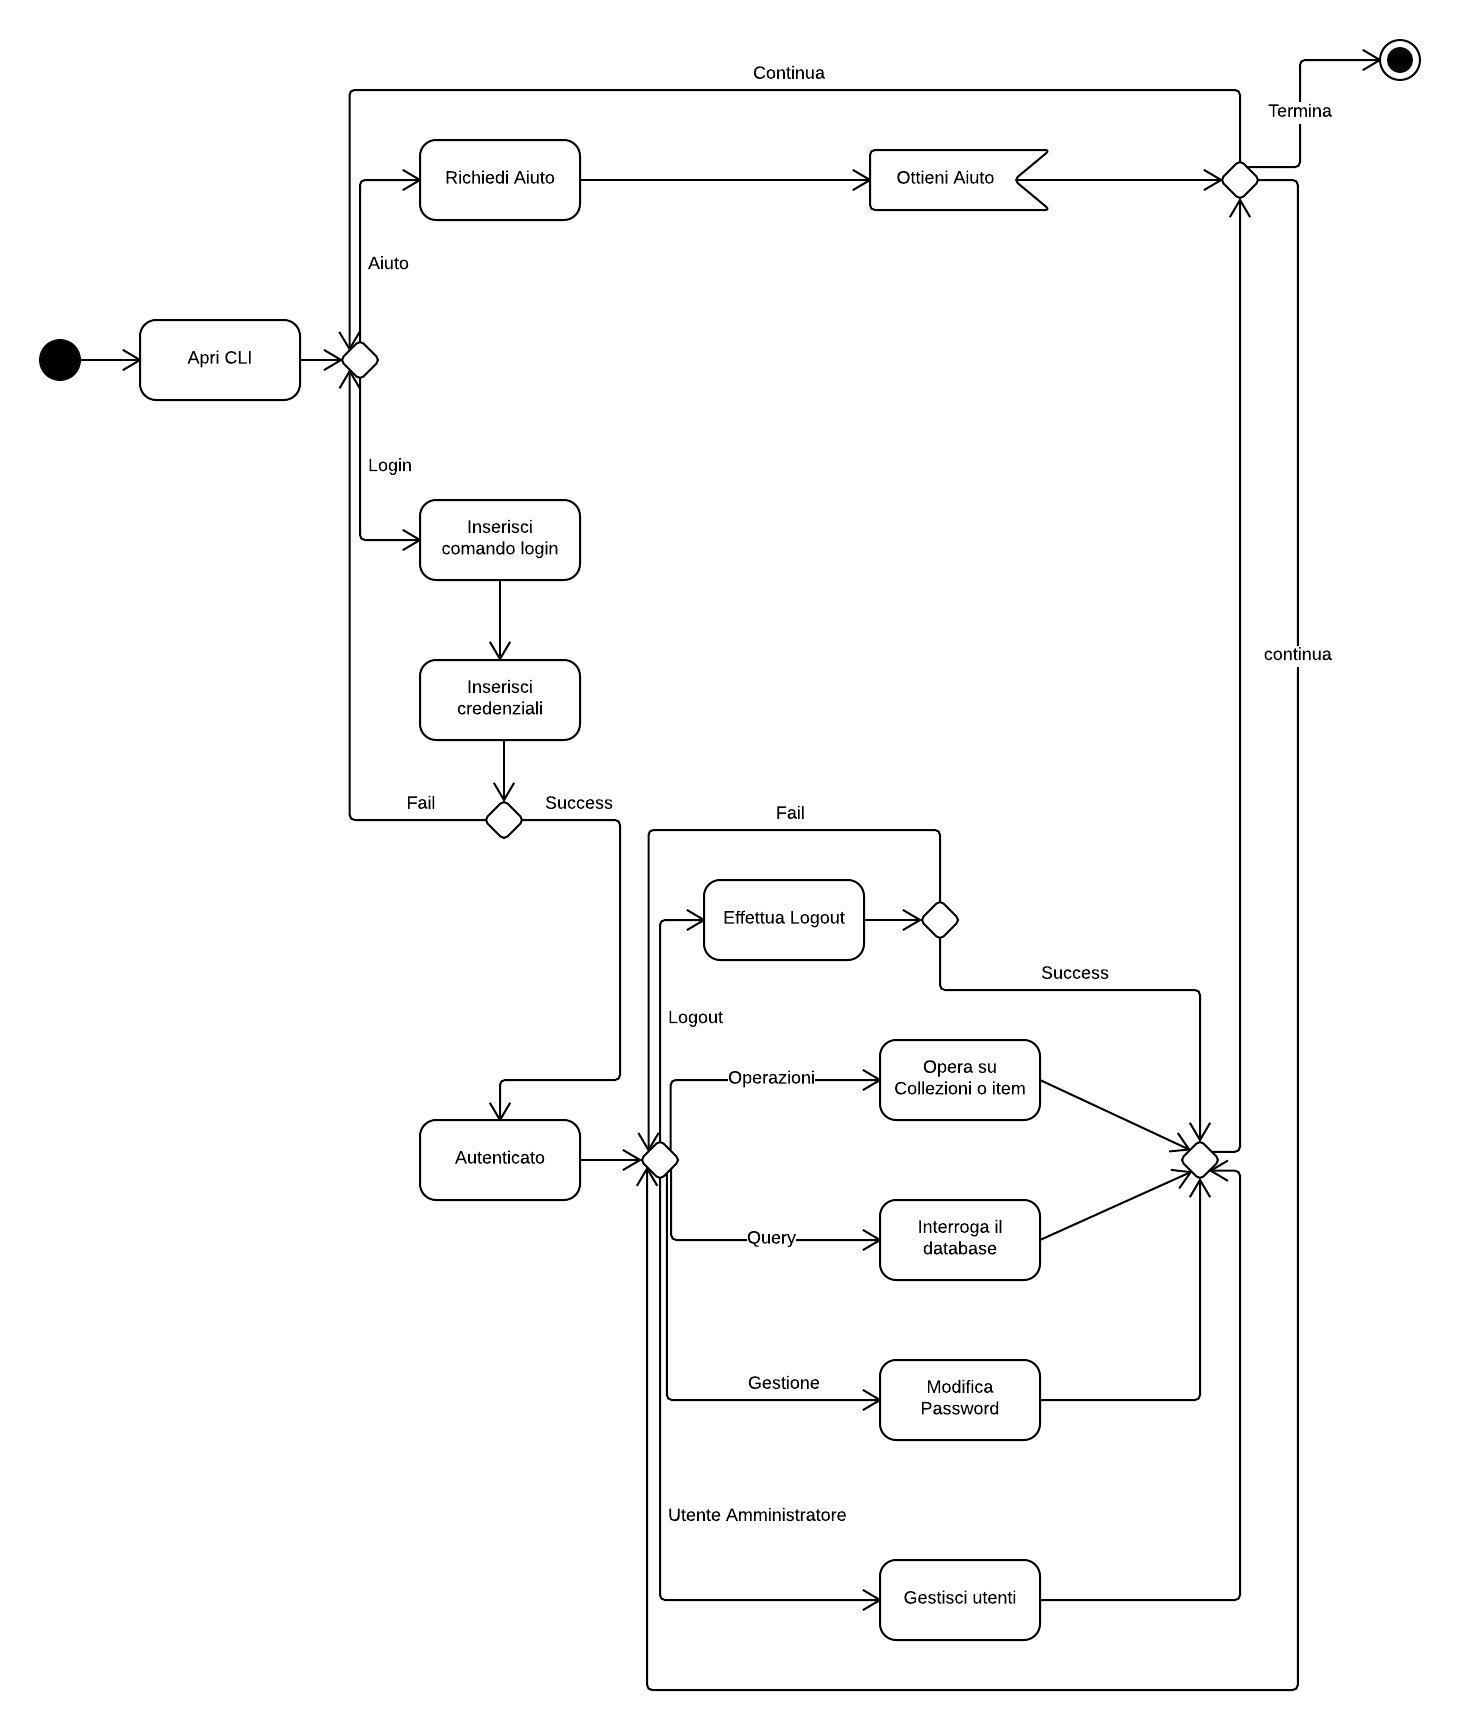
\includegraphics[width=0.8\textwidth, keepaspectratio]{img/diagrammiAttivita/visioneGenerale.jpeg}
    \caption{Diagrammi attività\ -\ Visione generale}
  \end{center}
\end{figure}

\subsection{Operazioni su collezioni e/o item}
\subsubsection{Creazione collezione}

Questo tipo di operazione permette di inserire una collezione all'interno del
\gloss{database}. Come si vede dal grafico che segue, l'utente dovrà inserire il
comando per la creazione della collezione, il nome della collezione stessa e i
suoi parametri. Una volta premuto il tasto invio, l'operazione andrà a buon
termine se l'utente ha scritto correttamente il comando altrimenti verrà
visualizzato un messaggio di errore.

\begin{figure}[H]
  \begin{center}
    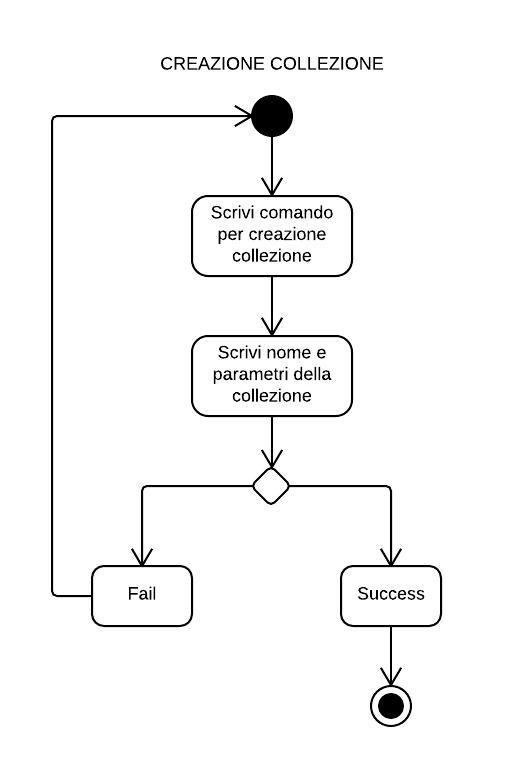
\includegraphics[width=0.3\textwidth, keepaspectratio]{img/diagrammiAttivita/creazioneCollezione.jpeg}
    \caption{Diagrammi attività\ -\ Creazione collezione}
  \end{center}
\end{figure}

\subsubsection{Cancellazione collezione}

Questo tipo di operazione permette di cancellare una collezione dal \gloss{database}.
Come si vede dal grafico che segue, l'utente dovrà inserire il comando per la
cancellazione di una collezione e il nome della collezione stessa. Una volta
premuto il tasto invio, l'operazione andrà a buon termine se l'utente ha
scritto correttamente il comando altrimenti verrà visualizzato un messaggio di
errore.

\begin{figure}[H]
  \begin{center}
    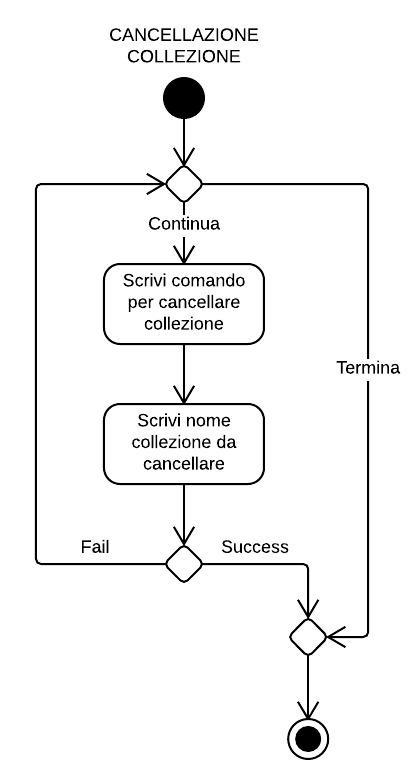
\includegraphics[width=0.3\textwidth, keepaspectratio]{img/diagrammiAttivita/cancCollezione.jpeg}
    \caption{Diagrammi attività\ -\ Cancellazione collezione}
  \end{center}
\end{figure}

\subsubsection{Visualizza collezioni}

Questo tipo di operazione permette di visualizzare le collezioni presenti
all'interno dal \gloss{database}. Come si vede dal grafico che segue, l'utente dovrà
inserire il comando per la visualizzazione delle collezioni. Una volta premuto
il tasto invio, l'operazione andrà a buon termine (ricevendo la lista delle
collezioni) se l'utente ha scritto correttamente il comando altrimenti verrà
visualizzato un messaggio di errore.

\begin{figure}[H]
  \begin{center}
    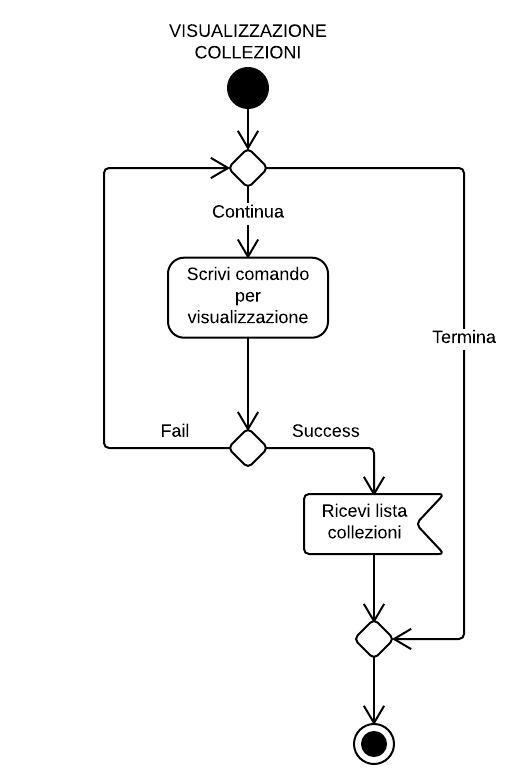
\includegraphics[width=0.3\textwidth, keepaspectratio]{img/diagrammiAttivita/visCollezione.jpeg}
    \caption{Diagrammi attività\ -\ Visualizzazione collezioni}
  \end{center}
\end{figure}

\subsubsection{Modifica nome collezione}

Questo tipo di operazione permette di modificare il nome di una collezione
presente nel \gloss{database}. Come si vede dal grafico che segue, l'utente dovrà
inserire il comando per la rinominazione della collezione, il nome della
collezione stessa e il nuovo nome per essa. Una volta premuto il tasto invio,
l'operazione andrà a buon termine se l'utente ha scritto correttamente il
comando altrimenti verrà visualizzato un messaggio di errore.

\begin{figure}[H]
  \begin{center}
    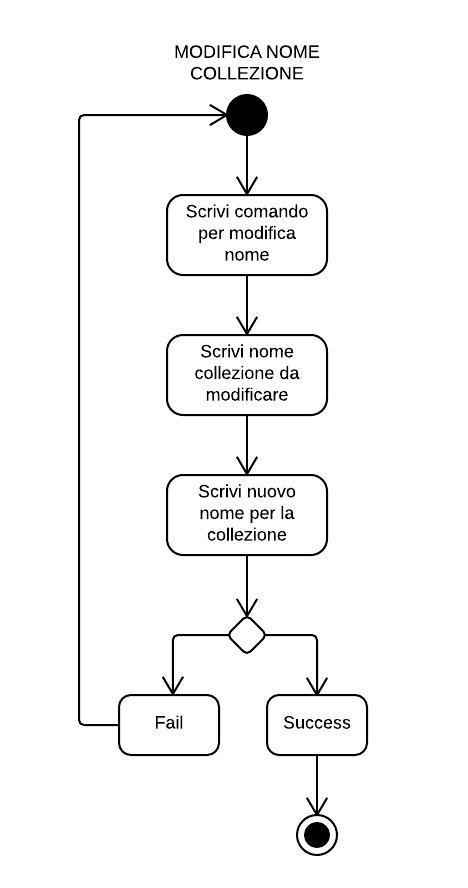
\includegraphics[width=0.3\textwidth, keepaspectratio]{img/diagrammiAttivita/modNomeCollezione.jpeg}
    \caption{Diagrammi attività - Modifica nome collezione}
  \end{center}
\end{figure}

\subsubsection{Inserimento item}

Questo tipo di operazione permette di inserire un item all'interno di una
collezione del \gloss{database}. Come si vede dal grafico che segue, l'utente dovrà
inserire il comando per l'inserimento item, il valore e parametri dell'item
stesso e il nome della collezione dove inserire l'item. Una volta premuto il
tasto invio, l'operazione andrà a buon termine (ricevendo la lista delle
collezioni) se l'utente ha scritto correttamente il comando altrimenti verrà
visualizzato un messaggio di errore.

\begin{figure}[H]
  \begin{center}
    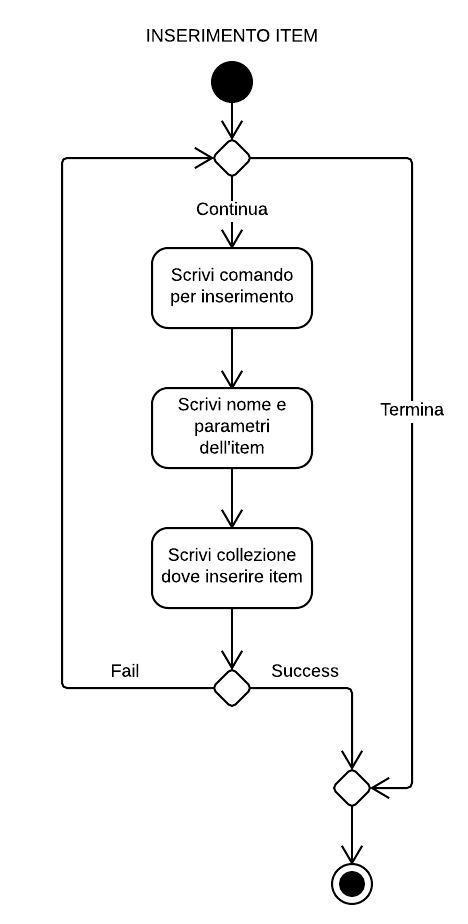
\includegraphics[width=0.3\textwidth, keepaspectratio]{img/diagrammiAttivita/inserimentoItem.jpeg}
    \caption{Diagrammi attività - Inserimento item}
  \end{center}
\end{figure}

\subsubsection{Rimozione item}

Questo tipo di operazione permette di rimuovere un item dall'interno di una
\gloss{collezione} del \gloss{database}. Come si vede dal grafico che segue, l'utente
dovrà inserire il comando per l'eliminazione di un item, il nome della
collezione da dove rimuovere l'item e il nome dell'item stesso. Una volta
premuto il tasto invio, l'operazione andrà a buon termine (ricevendo la lista
delle collezioni) se l'utente ha scritto correttamente il comando altrimenti
verrà visualizzato un messaggio di errore.

\begin{figure}[H]
  \begin{center}
    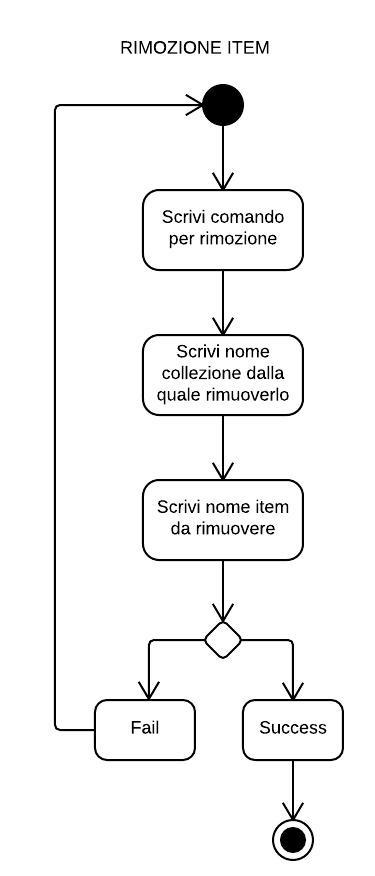
\includegraphics[width=0.3\textwidth, keepaspectratio]{img/diagrammiAttivita/rimozioneItem.jpeg}
    \caption{Diagrammi attività\ -\ Rimozione item}
  \end{center}
\end{figure}

\subsubsection{Aggiunta collaboratore}

Questo tipo di operazione permette di aggiungere un \gloss{collaboratore} ad
una collezione presente nel \gloss{database}. Come si vede dal grafico che segue,
l'utente dovrà inserire il comando per l'aggiunta di un collaboratore ad una
collezione, lo username del collaboratore e il nome della collezione alla
quale aggiungerlo. Una volta premuto il tasto invio, l'operazione andrà a buon
termine se l'utente ha scritto correttamente il comando altrimenti verrà
visualizzato un messaggio di errore.

\begin{figure}[H]
  \begin{center}
    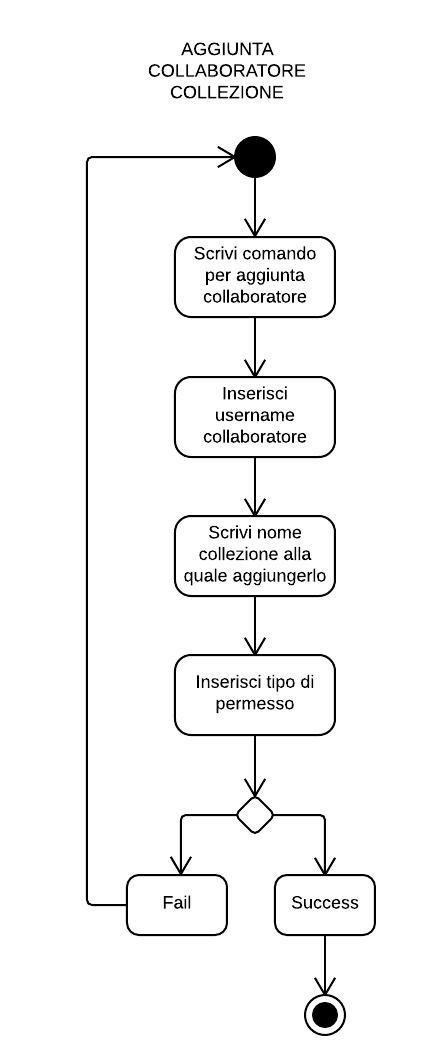
\includegraphics[width=0.3\textwidth, keepaspectratio]{img/diagrammiAttivita/aggCollaboratore.jpeg}
    \caption{Diagrammi attività\ -\ Aggiunta collaboratore}
  \end{center}
\end{figure}

\subsubsection{Rimozione collaboratore}

Questo tipo di operazione permette di rimuovere un collaboratore da una
collezione presente nel \gloss{database}. Come si vede dal grafico che segue, l'utente
dovrà inserire il comando per la rimozione di un collaboratore da una
collezione, lo username del collaboratore e il nome della collezione dalla
quale rimuoverlo. Una volta premuto il tasto invio, l'operazione andrà a buon
termine se l'utente ha scritto correttamente il comando altrimenti verrà
visualizzato un messaggio di errore.

\begin{figure}[H]
  \begin{center}
    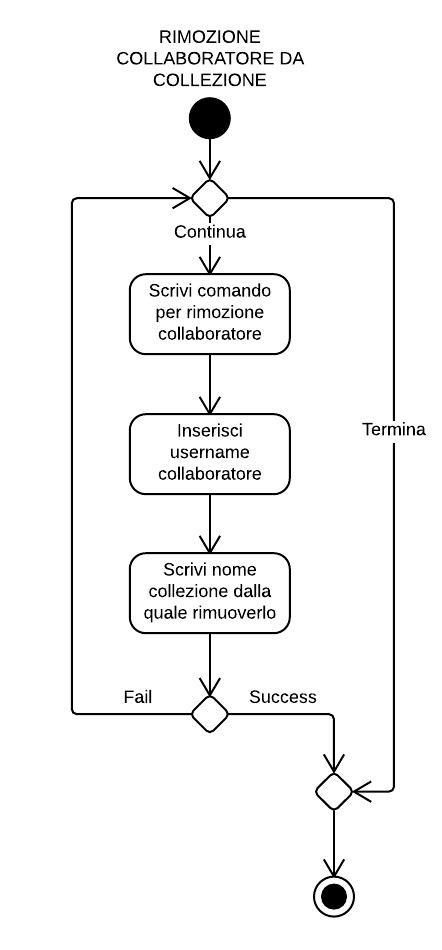
\includegraphics[width=0.3\textwidth, keepaspectratio]{img/diagrammiAttivita/rimozioneCollaboratore.jpeg}
    \caption{Diagrammi attività\ -\ Rimozione collaboratore}
  \end{center}
\end{figure}

\subsubsection{Import}

Questo tipo di operazione permette di importare nel \gloss{database} collezioni o item
tramite file \gloss{JSON}. Come si vede dal grafico che segue, l'utente dovrà
inserire il comando per l'importazione e il path che porta al file desiderato.
Una volta premuto il tasto invio, l'operazione andrà a buon termine se
l'utente ha scritto correttamente il comando altrimenti verrà visualizzato un
messaggio di errore.

\begin{figure}[H]
  \begin{center}
    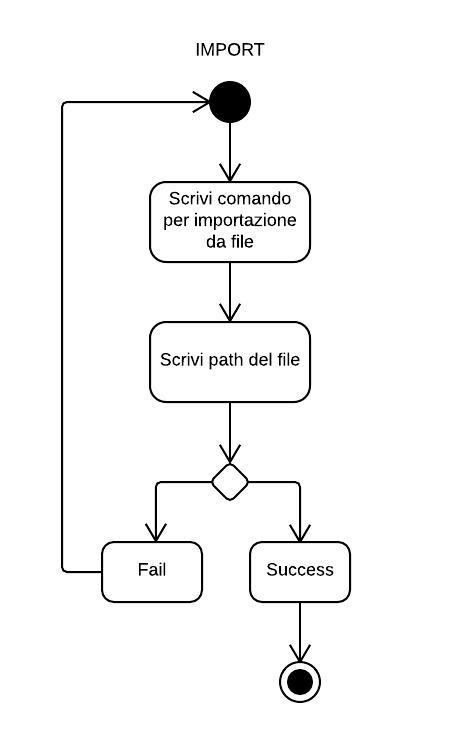
\includegraphics[width=0.3\textwidth, keepaspectratio]{img/diagrammiAttivita/import.jpeg}
    \caption{Diagrammi attività - Import}
  \end{center}
\end{figure}

\subsection{Interrogazione del database}

Questo tipo di operazione permette di interrogare il \gloss{database} tramite delle
query. Come si vede dal grafico che segue, l'utente dovrà inserire il comando
per l'interrogazione del \gloss{database} e i parametri per la ricerca. Una volta
premuto il tasto invio, l'operazione andrà a buon termine se l'utente ha
scritto correttamente il comando, ricevendo il risultato della query,
altrimenti verrà visualizzato un messaggio di errore.

\begin{figure}[H]
  \begin{center}
    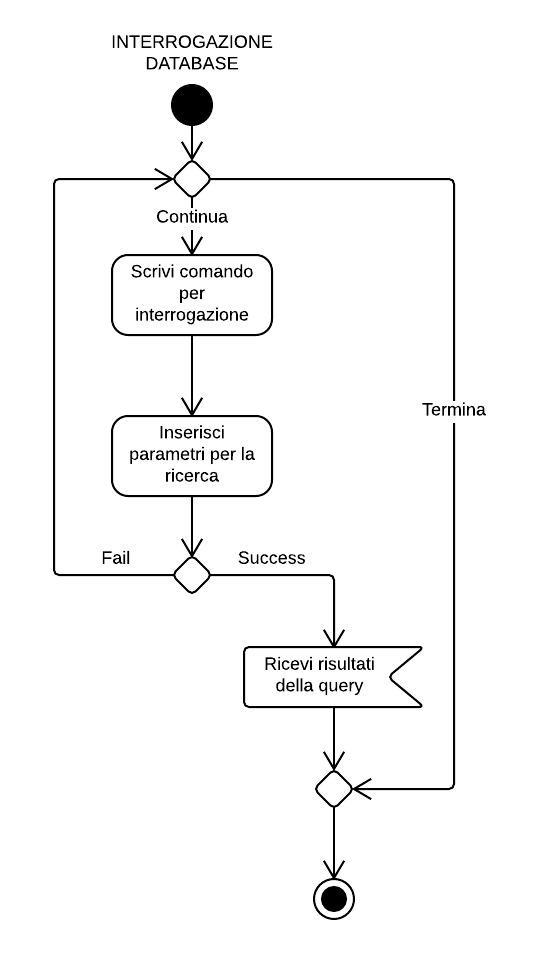
\includegraphics[width=0.3\textwidth, keepaspectratio]{img/diagrammiAttivita/query.jpeg}
    \caption{Diagrammi attività - Interrogazione del \gloss{database}}
  \end{center}
\end{figure}

\subsection{Modifica password}

Questo tipo di operazione permette di modificare la propria password. Come si
vede dal grafico che segue, l'utente dovrà inserire il comando per la modifica
della password, la vecchia password, la nuova password e confermare
quest'ultima. Una volta premuto il tasto invio, l'operazione andrà a buon
termine se l'utente ha scritto correttamente il comando altrimenti verrà
visualizzato un messaggio di errore.

\begin{figure}[H]
  \begin{center}
    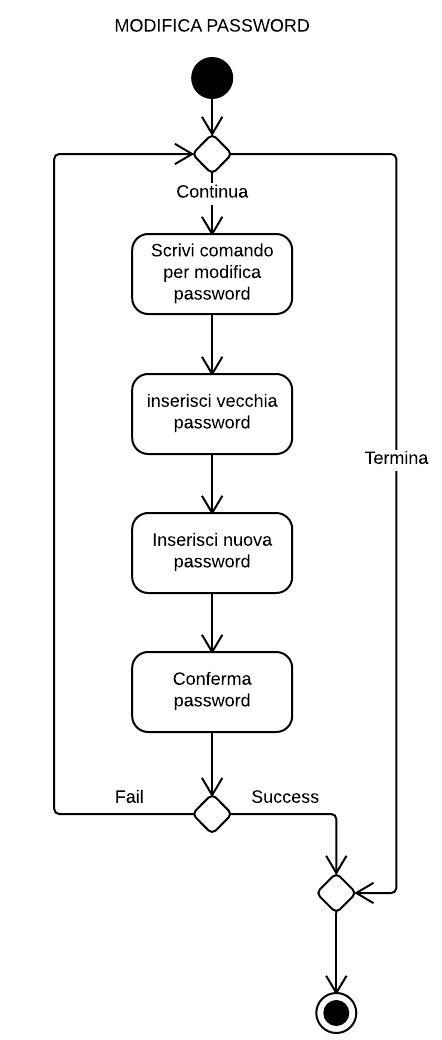
\includegraphics[width=0.3\textwidth, keepaspectratio]{img/diagrammiAttivita/modificaPsw.jpeg}
    \caption{Diagrammi attività - Modifica password}
  \end{center}
\end{figure}

\subsection{Gestione utenti}

La gestione utenti, possibile solo ad un utente amministratore, prevede la
possibilità di aggiungere o rimuovere un utente dal \gloss{database} e la possibilità
di resettare la password di un utente. Per aggiungere o rimuovere un utente,
l'amministratore dovrà inserire il rispettivo comando, lo username dell'utente
da aggiungere/rimuovere dal \gloss{database} e una conferma. Per resettare la password
di un utente, l'amministratore dovrà scrivere il comando per il reset della
password, lo username dell'utente interessato e una conferma. Una volta
premuto il tasto invio, le operazione andranno a buon termine se l'utente ha
scritto correttamente il comando altrimenti verrà visualizzato un messaggio di
errore.

\begin{figure}[H]
  \begin{center}
    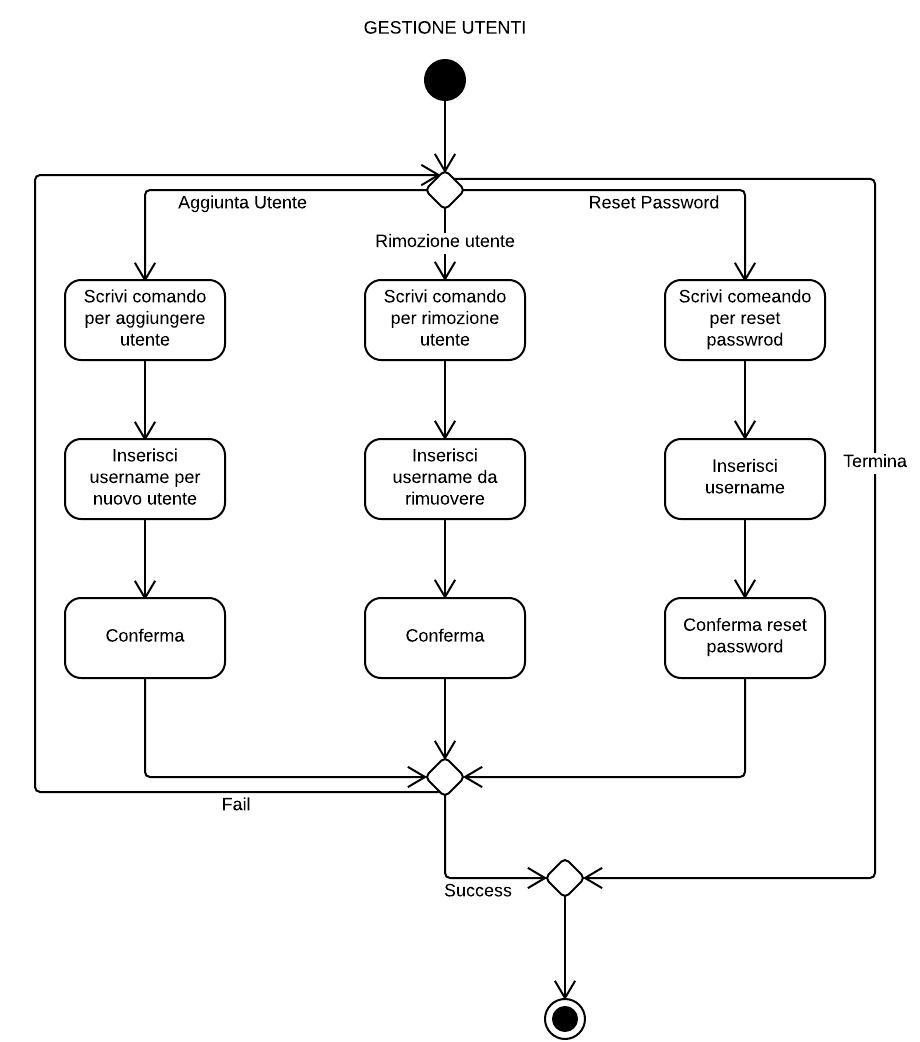
\includegraphics[width=0.9\textwidth, keepaspectratio]{img/diagrammiAttivita/gestioneUtenti.jpeg}
    \caption{Diagrammi attività - Gestione utenti}
  \end{center}
\end{figure}

\section{Design Pattern}

I \gloss{Design Pattern} rappresentano soluzioni progettuali generali ad un
problema ricorrente. Si tratta di  modelli logici da applicare per la
risoluzione di un problema ancor prima della definizione dell'algoritmo
risolutivo vero e proprio, favoriscono il riutilizzo del codice e rendono
l'architettura più manutenibile.\\
I \gloss{Design Pattern} possono essere suddivisi in:

\begin{itemize}
\item \textbf{architetturali:} operano al livello più alto,
  esprimono schemi di base per impostare l'organizzazione strutturale di un
  sistema software;
\item \textbf{creazionali:} nascondono i costruttori delle classi e mettono dei
  metodi al loro posto creando un'interfaccia, in questo modo forniscono
  un'astrazione del processo di instanziazione degli oggetti;
\item \textbf{strutturali:} consentono di riutilizzare degli oggetti esistenti
  fornendo agli utilizzatori un'interfaccia più adatta alle loro esigenze;
\item \textbf{comportamentali:} definiscono soluzioni per le interazioni tra
  oggetti.
\end{itemize}

Si rimanda all'Appendice A per un approfondimento dei \gloss{Design Pattern}
utilizzati nel progetto \textbf{Actorbase}.

\subsection{Design Pattern Architetturali}

\subsubsection{MVC}

\begin{itemize}
\item \textbf{Scopo:} È stato scelto l'utilizzo del pattern \gloss{Model}
  \gloss{View} \gloss{Controller} (\gloss{MVC}) per l'alto grado di separazione
  tra la parte logica dell'applicazione e parte grafica che offre;
\item \textbf{Utilizzo:} Viene utilizzato per delineare l'architettura generale
  della componente \gloss{CLI} (Command Line Interface) del progetto. La parte
  \gloss{View} funge da interfaccia con l'utente, si occupa di leggere l'input e
  inviarlo al Controller, il quale si occupa di validare l'input
  e inviare il comando estrapolato al \gloss{Model}.\\
  Il \gloss{Model} mediante un \gloss{Command Pattern} (vedi~\hyperref[sec:CommandPattern]{Command Pattern})
  esegue il comando richiesto e notifica la \gloss{View} utilizzando un \gloss{Observer Pattern}
  (vedi~\hyperref[sec:ObserverPattern]{Observer Pattern}) secondo la variante \gloss{Push model}.
\end{itemize}

\subsubsection{Dependancy Injection}
\begin{itemize}
\item \textbf{Scopo:} Separa il comportamento di una componente dalla risoluzione
  delle sue dipendenze, offrendo un maggiore grado di astrazione;
\item \textbf{Utilizzo:} Viene utilizzato nella componente driver, più
  precisamente nella classe
  \hyperref[sec:actorbase::driver::ActorbaseServices]{ActorbaseServices},
  sfruttando la variante \gloss{cake-pattern} offerta dal linguaggio \gloss{Scala}
  per aggiungere dipendenze amministrative fornite da
  \hyperref[sec:actorbase::driver::ActorbaseAdminservices]{ActorbaseAdminServices}
  alla classe dedicata alle operazioni comuni. Tale \gloss{pattern} viene anche
  utilizzato nella classe \hyperref[sec:actorbase::driver::client::ActorbaseClient]{ActorbaseClient}
  per fornire crittografia \gloss{TLS/SSL} (Transport Layer Security / Secure Socket Layer) al \gloss{client}
  utilizzato per la connessione.

\end{itemize}

\subsection{Design Pattern Creazionali}
% TODO: ricontrollare Singletonnnno
\subsubsection{Singleton}

\begin{figure}[H]
  \begin{center}
    \includegraphics[width=0.3\textwidth, keepaspectratio]{img/RP/Singleton-Connection.png}
    \caption{Connection Singleton}
  \end{center}
\end{figure}

\begin{itemize}
\item \textbf{Scopo:} Viene utilizzato per le classi di cui è preferibile avere un'unica istanza
  durante l'esecuzione dell'applicazione;
\item \textbf{Utilizzo:} È stato utilizzato una sola volta per la classe di connessione all'interno
  della componente \gloss{driver}, in modo da offrire un unico punto di accesso al \gloss{server}.
\end{itemize}

\subsubsection{Builder}

\begin{itemize}
\item \textbf{Scopo:} Il pattern \gloss{Builder} viene usato per separare la
  costruzione di un oggetto complesso dalla sua rappresentazione. L'algoritmo di
  creazione dell'oggetto complesso è indipendente dalle varie parti che
  costituiscono l'oggetto e da come vengono assemblate. In questo modo è possibile
  costruire diverse rappresentazioni dell'oggetto utilizzando lo stesso oggetto
  \gloss{Builder}.

\item \textbf{Utilizzo:} Viene implementato all'interno della componente
  \gloss{driver}, precisamente dalla classe
  \hyperref[sec:actorbase::driver::client::api::RequestBuilder]{RequestBuilder} per
  la costruzione delle diverse richieste \gloss{HTTP} da inviare alla componente \gloss{server}.
\end{itemize}

\subsection{Design Pattern Strutturali}

\subsubsection{Decorator}

\begin{itemize}
\item \textbf{Scopo:} Il pattern \gloss{Decorator} viene usato per aggiungere dinamicamente
  nuove funzionalità ad oggetti già esistenti, e permette di estenderli più facilmente;

\item \textbf{Utilizzo:} Viene utilizzato all'interno della componente
  \gloss{driver}, precisamente dalla classe
  \hyperref[sec:actorbase::driver::client::ActorbaseClient]{ActorbaseClient} per
  aggiungere funzionalità di protezione \gloss{SSL/TLS} alla comnicazione
  \gloss{HTTP} con la componente \gloss{server}.
\end{itemize}

\subsection{Design Pattern Comportamentali}

\subsubsection{Command Pattern}

\label{sec:CommandPattern}

\begin{itemize}
\item \textbf{Scopo:} Viene utilizzato per separare l'implementazione di un'azione
  (\gloss{Receiver}) dal richiamante dell'azione stessa (\gloss{Invoker}).
\item \textbf{Utilizzo:} Viene utilizzato per la gestione dei comandi nella componente
  \gloss{CLI}, e funge da \gloss{Model} dell'architettura \gloss{MVC} utilizzata.\\
  Le classi che implementano i comandi realizzando l'interfaccia \verb=Command= sono:
  \begin{itemize}
  \item \verb=FindCommand=
  \item \verb=ListCommand=
  \item \verb=LoginCommand=
  \item \verb=LogoutCommand=
  \item \verb=HelpCommand=
  \item \verb=InsertItemCommand=
  \item \verb=RemoveItemCommand=
  \item \verb=RenameCollectionCommand=
  \item \verb=CreateCollectionCommand=
  \item \verb=ChangePasswordCommand=
  \item \verb=RemoveCollectionCommand=
  \item \verb=ImportCommand=
  \item \verb=ExportCommand=
  \item \verb=AddContributorCommand=
  \item \verb=RemoveContributorCommand=
  \item \verb=ResetPasswordCommand=
  \item \verb=AddUserCommand=
  \item \verb=RemoveUserCommand=
  \end{itemize}
\end{itemize}

La classe incaricata di eseguire i comandi è \verb=CommandReceiver=, invocata mediante
\verb=CommandInvoker=, utilizzando i parametri ricevuti dalla parte \gloss{Controller}
dell'architettura \gloss{MVC} scelta per la componente \gloss{CLI}.

\subsubsection{Observer Pattern}

\label{sec:ObserverPattern}

\begin{itemize}
\item \textbf{Scopo:} Viene utilizzato per tenere sotto controllo lo stato di diversi oggetti, ed è parte dell'implementazione
  del \gloss{Design Pattern} \gloss{MVC} con logica \gloss{push model}, il funzionamento si basa su meccanismi di callback.
\item \textbf{Utilizzo:} È stato utilizzato nella componente \gloss{CLI} del progetto in modo da ottenere una \gloss{view}
  auto-aggiornante sull'output prodotto dai comandi inviati alla componente \gloss{driver}.\\
  Più in dettaglio, la classe \verb=CommandInvoker= realizza l'interfaccia \verb=Observable= aggiungendo l'oggetto di tipo
  \verb=ResultView= alla propria lista di \gloss{observers}, all'esecuzione di ogni comando, notifica \verb=resultview=
  con l'output prodotto.
\end{itemize}

\section{Stime di fattibilità e di bisogno di risorse}

Durante la progettazione dell'architettura, oltre alle tecnologie e librerie
consigliate dal proponente, ne sono state ricercate e testate altre in modo da
poter usufruire di funzionalità già esistenti.\\ Dopo un iniziale orientamento
verso il \gloss{framework} \gloss{Spring}, più precisamente nella sua
derivazione \gloss{SpringShell}, in modo da poter generare una \gloss{CLI}
personalizzata, abbiamo deciso di rimanere su un'implementazione più leggera in
linguaggio \gloss{Scala} in quanto la scarsa personalizzazione offerta e il
grosso carico di dipendenze che necessitava \gloss{SpringShell} per il suo
utilizzo è stato ritenuto eccessivamente gravoso sulla realizzazione della
componente in questione.\\ È stato tuttavia deciso di utilizzare il
\gloss{framework} \gloss{pickling} per effettuare \gloss{serializzazione} della
persistenza su disco; offre una buona documentazione e numerosi esempi di
utilizzo, rende inoltre possibile la definizione di protocolli di
\gloss{serializzazione} personalizzati.\\
Per la gestione della comunicazione \gloss{HTTP} sono stati utilizzate due librerie:
\begin{itemize}
\item\textbf{Lato server:} Spray permette di gestire efficacemente le richieste in ingresso
  di tipo \gloss{HTTP} asincronamente, appositamente sviluppata per funzionare in congiunzione
  con il modello ad attori offerto da \gloss{akka};
\item\textbf{Lato client:} Scalaj-http è una semplice libreria \gloss{Scala} che funge da client
  \gloss{HTTP} per la comunicazione con la componente \gloss{server}.
\end{itemize}

\section{Tracciamento}

\subsection{Tracciamento Componenti-Requisiti}

\begin{longtable}[H]{|p{9cm}|p{8cm}|}
  \hline
  \textbf{Componente} & \textbf{Requisiti}\\
  \hline
  actorbase & \multiLineCell[t]{DEF3 DEV8\\DEV9 OBF1\\OBF2 OBQ12\\OBV4 OBV5\\OBV6 OBV7\\}\\
\hline
actorbase::actorsystem & \multiLineCell[t]{OBF1\\}\\
\hline
actorbase::actorsystem::clientactor & \multiLineCell[t]{OBF1.1.10 OBF1.1.10.1\\OBF1.1.10.1.1 OBF1.1.10.2\\OBF1.1.10.2.1 OBF1.1.10.2.1.1\\OBF1.1.10.2.2 OBF1.1.10.2.3\\OBF1.1.10.2.3.1 OBF1.1.10.2.3.2\\OBF1.1.10.2.4 OBF1.1.10.2.4.1\\OBF1.1.10.2.5 OBF1.1.10.2.5.1\\OBF1.1.10.2.5.2 OBF1.1.10.2.5.3\\OBF1.1.10.2.5.4 OBF1.1.10.2.6\\OBF1.1.10.2.6.1 OBF1.1.10.2.7\\OBF1.1.10.3 OBF1.1.10.3.1\\OBF1.1.10.3.2 OBF1.1.10.3.3\\OBF1.1.10.3.4 OBF1.1.10.3.5\\OBF1.1.10.4 OBF1.1.10.5\\OBF1.1.10.5.1 OBF1.1.10.6\\OBF1.1.10.7 OBF1.1.10.7.1\\OBF1.1.10.7.1.1 OBF1.1.10.7.2\\OBF1.1.10.7.2.1 OBF1.1.10.7.3\\OBF1.1.10.7.3.1 OBF1.1.2\\}\\
\hline
actorbase::actorsystem::clientactor::messages & \multiLineCell[t]{OBF1.1.2.1 OBF1.1.2.2\\}\\
\hline
actorbase::actorsystem::httpserver & \multiLineCell[t]{OBF1.1 OBF1.1.1\\OBF1.1.1.1 OBF1.1.10\\}\\
\hline
actorbase::actorsystem::httpserver::messages & \multiLineCell[t]{OBF1.1.1.1.1\\}\\
\hline
actorbase::actorsystem::main & \multiLineCell[t]{OBF1.1.10.1 OBF1.1.10.2\\OBF1.1.10.2.1 OBF1.1.10.2.1.1\\OBF1.1.10.2.3 OBF1.1.10.2.4\\OBF1.1.10.2.5 OBF1.1.10.2.5.1\\OBF1.1.10.2.5.2 OBF1.1.10.2.6\\OBF1.1.10.2.7 OBF1.1.10.3\\OBF1.1.10.3.1 OBF1.1.10.3.2\\OBF1.1.10.3.3 OBF1.1.10.3.4\\OBF1.1.10.4 OBF1.1.10.5\\OBF1.1.10.7 OBF1.1.10.7.1\\OBF1.1.10.7.2 OBF1.1.10.7.2.1\\OBF1.1.10.7.3 OBF1.1.10.7.3.1\\OBF1.1.3\\}\\
\hline
actorbase::actorsystem::main::messages & \multiLineCell[t]{OBF1.1.3.1 OBF1.1.3.2\\OBF1.1.3.3 OBF1.1.3.4\\OBF1.1.3.5 OBF1.1.3.6\\OBF1.1.3.7 OBF1.1.3.8\\OBF1.1.3.9 OBF1.1.3.11\\OBF1.1.3.12 OBF1.1.3.12\\OBF1.1.3.13}\\
\hline
actorbase::actorsystem::manager & \multiLineCell[t]{DEF1.1.8 OBF1.1.10.3\\OBF1.1.10.3.1\\}\\
\hline
actorbase::actorsystem::manager::messages & \multiLineCell[t]{DEF1.1.8.1 DEF1.1.8.2\\}\\
\hline
actorbase::actorsystem::ninja & \multiLineCell[t]{DEF1.1.7 OBF1.1.10.2\\OBF1.1.10.2.4 OBF1.1.10.2.5\\OBF1.1.10.2.5.1 OBF1.1.10.2.5.2\\OBF1.1.10.2.6 OBF1.1.10.2.7\\OBF1.1.10.3 OBF1.1.10.3.1\\OBF1.1.10.3.4\\}\\
\hline
actorbase::actorsystem::ninja::messages & \multiLineCell[t]{DEF1.1.7.1 DEF1.1.7.2\\}\\
\hline
actorbase::actorsystem::storefinder & \multiLineCell[t]{OBF1.1.10.1 OBF1.1.10.2\\OBF1.1.10.2.1 OBF1.1.10.2.3\\OBF1.1.10.2.4 OBF1.1.10.2.5\\OBF1.1.10.2.5.1 OBF1.1.10.2.5.2\\OBF1.1.10.2.5.4 OBF1.1.10.2.6\\OBF1.1.10.2.7 OBF1.1.10.3\\OBF1.1.10.3.1 OBF1.1.10.3.3\\OBF1.1.10.3.4 OBF1.1.10.4\\OBF1.1.10.5 OBF1.1.10.7\\OBF1.1.10.7.1 OBF1.1.10.7.2\\OBF1.1.10.7.2.1 OBF1.1.10.7.3\\OBF1.1.10.7.3.1 OBF1.1.4\\}\\
\hline
actorbase::actorsystem::storefinder::messages & \multiLineCell[t]{OBF1.1.4.1 OBF1.1.4.2\\OBF1.1.4.3 OBF1.1.4.4\\OBF1.1.4.5 OBF1.1.4.6\\OBF1.1.4.7}\\
\hline
actorbase::actorsystem::storekeeper & \multiLineCell[t]{OBF1.1.10.2 OBF1.1.10.2.1\\OBF1.1.10.2.4 OBF1.1.10.2.5\\OBF1.1.10.2.5.1 OBF1.1.10.2.5.2\\OBF1.1.10.2.6 OBF1.1.10.2.7\\OBF1.1.10.3 OBF1.1.10.3.1\\OBF1.1.10.3.3 OBF1.1.10.3.4\\OBF1.1.10.4 OBF1.1.5\\}\\
\hline
actorbase::actorsystem::storekeeper::messages & \multiLineCell[t]{OBF1.1.5.1 OBF1.1.5.2\\OBF1.1.5.3 OBF1.1.5.4\\OBF1.1.5.5 OBF1.1.5.6\\OBF1.1.5.7}\\
\hline
actorbase::actorsystem::userfinder & \multiLineCell[t]{OBF1.1.10.1 OBF1.1.10.1.1\\OBF1.1.10.2 OBF1.1.10.2.1\\OBF1.1.10.2.3 OBF1.1.10.2.3.1\\OBF1.1.10.2.4 OBF1.1.10.2.5\\OBF1.1.10.2.5.1 OBF1.1.10.2.5.2\\OBF1.1.10.2.6 OBF1.1.10.2.7\\OBF1.1.10.3 OBF1.1.10.3.2\\OBF1.1.10.5 OBF1.1.10.5.1\\OBF1.1.10.7 OBF1.1.10.7.1\\OBF1.1.10.7.3 OBF1.1.11\\}\\
\hline
actorbase::actorsystem::userfinder::messages & \multiLineCell[t]{OBF1.1.11.1 OBF1.1.11.2\\OBF1.1.11.3 OBF1.1.11.4\\OBF1.1.11.5 OBF1.1.11.6\\OBF1.1.11.7\\}\\
\hline
actorbase::actorsystem::userkeeper & \multiLineCell[t]{OBF1.1.10.1 OBF1.1.10.1.1\\OBF1.1.10.2 OBF1.1.10.2.1\\OBF1.1.10.2.3 OBF1.1.10.2.3.1\\OBF1.1.10.2.4 OBF1.1.10.2.5\\OBF1.1.10.2.5.1 OBF1.1.10.2.5.2\\OBF1.1.10.2.6 OBF1.1.10.2.7\\OBF1.1.10.3 OBF1.1.10.3.2\\OBF1.1.10.5 OBF1.1.10.5.1\\OBF1.1.10.7 OBF1.1.10.7.1\\OBF1.1.10.7.3 OBF1.1.9\\}\\
\hline
actorbase::actorsystem::userkeeper::messages & \multiLineCell[t]{OBF1.1.9.1 OBF1.1.9.2\\OBF1.1.9.3 OBF1.1.9.4\\OBF1.1.9.5 OBF1.1.9.6\\OBF1.1.9.9}\\
\hline
actorbase::actorsystem::utils & \multiLineCell[t]{DEF1.1.7 OBF1.1.11\\OBF1.1.2 OBF1.1.3\\OBF1.1.4 OBF1.1.5\\OBF1.1.6 OBF1.1.9\\}\\
\hline
actorbase::actorsystem::warehouseman & \multiLineCell[t]{OBF1.1.10.2 OBF1.1.10.2.4\\OBF1.1.10.2.5 OBF1.1.10.2.5.1\\OBF1.1.10.2.5.2 OBF1.1.10.2.6\\OBF1.1.10.2.7 OBF1.1.10.3\\OBF1.1.10.3.1 OBF1.1.10.3.4\\OBF1.1.6\\}\\
\hline
actorbase::actorsystem::warehouseman::messages & \multiLineCell[t]{OBF1.1.6.1 OBF1.1.6.2\\OBF1.1.6.3 OBF1.1.6.4\\}\\
\hline
actorbase::cli & \multiLineCell[t]{OBF2\\}\\
\hline
actorbase::cli::controllers & \multiLineCell[t]{DEF2.1.2.7 DEF2.1.3.1.2\\DEF2.1.4 DEF2.1.5\\OBF2.1 OBF2.1.1\\OBF2.1.2 OBF2.1.2.1\\OBF2.1.2.2 OBF2.1.2.3\\OBF2.1.2.4 OBF2.1.2.5\\OBF2.1.2.6 OBF2.1.3\\OBF2.1.3.1 OBF2.1.3.1.1\\OBF2.1.6 OBF2.1.7\\OBF2.1.8 OBF2.1.9\\OBF2.1.9.1 OBF2.1.9.2\\OBF2.1.9.3\\}\\
\hline
actorbase::cli::models & \multiLineCell[t]{DEF2.1.2.7 DEF2.1.2.7.1\\DEF2.1.3.1.2 DEF2.1.3.1.2.1\\DEF2.1.4 DEF2.1.5\\DEF2.1.5.1 OBF2.1.1\\OBF2.1.1.1 OBF2.1.1.2\\OBF2.1.2 OBF2.1.2.1\\OBF2.1.2.1.1 OBF2.1.2.2\\OBF2.1.2.3 OBF2.1.2.3.1\\OBF2.1.2.4 OBF2.1.2.4.1\\OBF2.1.2.4.2 OBF2.1.2.5\\OBF2.1.2.5.1 OBF2.1.2.5.2\\OBF2.1.2.5.3 OBF2.1.2.6\\OBF2.1.2.6.1 OBF2.1.2.6.2\\OBF2.1.2.8 OBF2.1.3\\OBF2.1.3.1 OBF2.1.3.1.1\\OBF2.1.3.1.1.1 OBF2.1.3.1.1.2\\OBF2.1.3.1.1.3 OBF2.1.3.1.1.4\\OBF2.1.3.1.1.5 OBF2.1.3.6 OBF2.1.6\\OBF2.1.6.1 OBF2.1.6.2\\OBF2.1.7 OBF2.1.7.1\\OBF2.1.7.2 OBF2.1.7.3\\OBF2.1.8 OBF2.1.9\\OBF2.1.9.1 OBF2.1.9.1.1\\OBF2.1.9.1.2 OBF2.1.9.2\\OBF2.1.9.2.1 OBF2.1.9.2.2\\OBF2.1.9.3 OBF2.1.9.3.1\\OBF2.1.9.3.2\\}\\
\hline
actorbase::cli::views & \multiLineCell[t]{DEF2.1.2.7 DEF2.1.2.7.1 DEF2.1.2.7.2\\DEF2.1.3.1.2 DEF2.1.3.1.2.1\\DEF2.1.3.2 DEF2.1.3.3\\DEF2.1.4 DEF2.1.5\\DEF2.1.5.1 OBF2\\OBF2.1.1 OBF2.1.1.1\\OBF2.1.1.2 OBF2.1.1.3\\OBF2.1.2 OBF2.1.2.1\\OBF2.1.2.1.1 OBF2.1.2.10\\OBF2.1.2.11 OBF2.1.2.12\\OBF2.1.2.13 OBF2.1.2.14\\OBF2.1.2.2 OBF2.1.2.3\\OBF2.1.2.3.1 OBF2.1.2.4\\OBF2.1.2.4.1 OBF2.1.2.4.2\\OBF2.1.2.5 OBF2.1.2.5.1\\OBF2.1.2.5.2 OBF2.1.2.5.3\\OBF2.1.2.6 OBF2.1.2.6.1\\OBF2.1.2.6.2 OBF2.1.2.8\\OBF2.1.2.9 OBF2.1.3\\OBF2.1.3.1 OBF2.1.3.1.1\\OBF2.1.3.1.1.1 OBF2.1.3.1.1.2\\OBF2.1.3.1.1.3 OBF2.1.3.1.1.4\\OBF2.1.3.1.1.5 OBF2.1.3.4\\OBF2.1.3.6 OBF2.1.3.6.1\\OBF2.1.3.6.2\\OBF2.1.3.5 OBF2.1.6\\OBF2.1.6.1 OBF2.1.6.2\\OBF2.1.7 OBF2.1.7.1\\OBF2.1.7.2 OBF2.1.7.3\\OBF2.1.7.4 OBF2.1.7.5\\OBF2.1.7.6 OBF2.1.8\\OBF2.1.9 OBF2.1.9.1\\OBF2.1.9.1.1 OBF2.1.9.1.2\\OBF2.1.9.2 OBF2.1.9.2.1\\OBF2.1.9.2.2 OBF2.1.9.3\\OBF2.1.9.3.1 OBF2.1.9.3.2\\OBF2.1.9.4 OBF2.1.9.5\\OBF2.1.9.6\\}\\
\hline
actorbase::cli::views::Observer & \multiLineCell[t]{DEF3.1.2 DEF3.1.3\\OBF2.1.2.10 OBF2.1.2.11\\OBF2.1.2.12 OBF2.1.2.13\\OBF2.1.2.14 OBF2.1.2.8\\OBF2.1.2.9 OBF2.1.3.4\\OBF2.1.3.5 OBF2.1.7.4\\OBF2.1.7.5 OBF2.1.7.6\\OBF2.1.9.4 OBF2.1.9.5\\OBF2.1.9.6\\}\\
\hline
actorbase::driver & \multiLineCell[t]{DEF3\\}\\
\hline
actorbase::driver::client & \multiLineCell[t]{DEF3.1 DEF3.1.1\\DEF3.1.2 DEF3.1.3\\DEF3.2 DEF3.2.1\\DEF3.2.1.1 DEF3.2.1.2\\DEF3.2.2 DEF3.2.3\\DEF3.2.3.1 DEF3.2.3.2\\DEF3.2.4 DEF3.2.4.1\\DEF3.2.4.2 DEF3.2.4.3\\DEF3.2.4.4 DEF3.2.5\\DEF3.2.5.1 DEF3.2.5.2\\DEF3.2.5.3 DEF3.2.5.4\\DEF3.2.5.5 DEF3.2.6\\DEF3.2.6.1 DEF3.2.6.2\\DEF3.2.6.3 DEF3.2.7\\DEF3.2.7.1 DEF3.2.7.2\\DEF3.2.7.3 DEF3.3\\DEF3.3.1 DEF3.3.1.1\\DEF3.3.1.1.1 DEF3.3.1.1.2\\DEF3.3.1.1.3 DEF3.3.1.1.4\\DEF3.3.1.2 DEF3.3.1.2.1\\DEF3.3.1.2.2 DEF3.3.1.2.3\\DEF3.3.1.4 DEF3.3.2\\DEF3.3.2.1 DEF3.3.2.2\\DEF3.3.2.3 DEF3.4\\DEF3.4.1 DEF3.4.2\\DEF3.5 DEF3.6\\DEF3.6.1 DEF3.6.1.1\\DEF3.6.2 DEF3.6.2.1\\DEF3.6.3 DEF3.6.3.1\\DEF3.6.4 DEF3.6.5\\DEF3.6.6 DEF3.7\\DEF3.7.1 DEF3.7.2\\DEF3.7.3 DEF3.7.4\\DEF3.8 DEF3.8.1\\DEF3.8.2 DEF3.8.3\\}\\
\hline
actorbase::driver::client::api & \multiLineCell[t]{DEF3.1 DEF3.1.1\\DEF3.1.2 DEF3.2\\DEF3.2.1 DEF3.2.1.1\\DEF3.2.2 DEF3.2.3\\DEF3.2.3.1 DEF3.2.4\\DEF3.2.4.1 DEF3.2.4.2\\DEF3.2.5 DEF3.2.5.1\\DEF3.2.5.2 DEF3.2.5.5\\DEF3.2.6 DEF3.2.6.1\\DEF3.2.6.2 DEF3.2.7\\DEF3.2.7.1 DEF3.2.7.2\\DEF3.2.7.3 DEF3.3\\DEF3.3.1 DEF3.3.1.1\\DEF3.3.1.1.1 DEF3.3.1.1.2\\DEF3.3.1.1.3 DEF3.3.1.1.4\\DEF3.3.1.2 DEF3.3.1.2.1\\DEF3.3.2 DEF3.3.2.1\\DEF3.3.2.2 DEF3.4\\DEF3.4.1 DEF3.4.2\\DEF3.5 DEF3.6\\DEF3.6.1 DEF3.6.1.1\\DEF3.6.2 DEF3.6.2.1\\DEF3.6.3 DEF3.6.3.1\\DEF3.7 DEF3.7.1\\DEF3.7.2\\}\\
\hline
actorbase::driver::data & \multiLineCell[t]{DEF3.2 DEF3.2.1\\DEF3.2.1.1 DEF3.2.1.2\\DEF3.2.3 DEF3.2.3.1\\DEF3.2.4 DEF3.2.4.1\\DEF3.2.4.2 DEF3.2.4.3\\DEF3.2.4.4 DEF3.2.5\\DEF3.2.5.1 DEF3.2.5.2\\DEF3.2.5.3 DEF3.2.5.4\\DEF3.2.5.5 DEF3.2.6\\DEF3.2.6.1 DEF3.2.6.2\\DEF3.2.6.3 DEF3.3\\DEF3.3.1 DEF3.3.1.1\\DEF3.3.1.1.1 DEF3.3.1.1.2\\DEF3.3.1.1.3 DEF3.3.1.1.4\\DEF3.3.1.4 DEF3.3.2\\DEF3.3.2.1 DEF3.3.2.2\\DEF3.3.2.3 DEF3.4\\DEF3.4.1 DEF3.4.2\\DEF3.8 DEF3.8.1\\DEF3.8.2 DEF3.8.3\\}\\
\hline
actorbase::driver::exceptions & \multiLineCell[t]{DEF3.1.3 DEF3.2.1.2\\DEF3.2.3.2 DEF3.2.4.3\\DEF3.2.4.4 DEF3.2.5.3\\DEF3.2.5.4 DEF3.2.6.3\\DEF3.3.1.2.2 DEF3.3.1.2.3\\DEF3.3.1.4 DEF3.3.2.3\\DEF3.6.4 DEF3.6.5\\DEF3.6.6 DEF3.7.3\\DEF3.7.4\\}\\
\hline
\end{longtable}




\subsection{Tracciamento Requisiti-Componenti}
\begin{longtable}[H]{|p{6cm}|p{11cm}|}
  \hline
  \textbf{Requisito} & \textbf{Componenti}\\
\hline
DEF1.1.7 & \multiLineCell[t]{actorbase::actorsystem::ninja\\actorbase::actorsystem::utils\\}\\
\hline
DEF1.1.7.1 & \multiLineCell[t]{actorbase::actorsystem::ninja::messages\\}\\
\hline
DEF1.1.7.2 & \multiLineCell[t]{actorbase::actorsystem::ninja::messages\\}\\
\hline
DEF1.1.8 & \multiLineCell[t]{actorbase::actorsystem::manager\\}\\
\hline
DEF1.1.8.1 & \multiLineCell[t]{actorbase::actorsystem::manager::messages\\}\\
\hline
DEF1.1.8.2 & \multiLineCell[t]{actorbase::actorsystem::manager::messages\\}\\
\hline
DEF2.1.2.7 & \multiLineCell[t]{actorbase::cli::models\\actorbase::cli::views\\}\\
\hline
DEF2.1.2.7.1 & \multiLineCell[t]{actorbase::cli::models\\actorbase::cli::views\\}\\
\hline
%DEF2.1.2.7.2 & \multiLineCell[t]{C14ss3::actorbase::cli::views::CommandLoop\\}\\
%\hline
DEF2.1.2.7.2 & \multiLineCell[t]{actorbase::cli::views\\}\\
\hline
DEF2.1.3.1.2 & \multiLineCell[t]{actorbase::cli::controllers\\actorbase::cli::models\\actorbase::cli::views\\}\\
\hline
DEF2.1.3.1.2.1 & \multiLineCell[t]{actorbase::cli::models\\actorbase::cli::views\\}\\
\hline
DEF2.1.3.2 & \multiLineCell[t]{actorbase::cli::views\\}\\
\hline
DEF2.1.3.3 & \multiLineCell[t]{actorbase::cli::views\\}\\
\hline
DEF2.1.4 & \multiLineCell[t]{actorbase::cli::controllers\\actorbase::cli::models\\actorbase::cli::views\\}\\
\hline
DEF2.1.5 & \multiLineCell[t]{actorbase::cli::controllers\\actorbase::cli::models\\actorbase::cli::views\\}\\
\hline
DEF2.1.5.1 & \multiLineCell[t]{actorbase::cli::models\\actorbase::cli::views\\}\\
\hline
DEF3 & \multiLineCell[t]{actorbase\\actorbase::driver\\}\\
\hline
DEF3.1 & \multiLineCell[t]{actorbase::driver::client\\actorbase::driver::client::api\\}\\
\hline
DEF3.1.1 & \multiLineCell[t]{actorbase::driver::client\\actorbase::driver::client::api\\}\\
\hline
DEF3.1.2 & \multiLineCell[t]{actorbase::cli::views::Observer\\actorbase::driver::client\\actorbase::driver::client::api\\}\\
\hline
DEF3.1.3 & \multiLineCell[t]{actorbase::cli::views::Observer\\actorbase::driver::client\\actorbase::driver::exceptions\\}\\
\hline
DEF3.2 & \multiLineCell[t]{actorbase::driver::client\\actorbase::driver::client::api\\actorbase::driver::data\\}\\
\hline
DEF3.2.1 & \multiLineCell[t]{actorbase::driver::client\\actorbase::driver::client::api\\actorbase::driver::data\\}\\
\hline
DEF3.2.1.1 & \multiLineCell[t]{actorbase::driver::client\\actorbase::driver::client::api\\actorbase::driver::data\\}\\
\hline
DEF3.2.1.2 & \multiLineCell[t]{actorbase::driver::client\\actorbase::driver::data\\actorbase::driver::exceptions\\}\\
\hline
DEF3.2.2 & \multiLineCell[t]{actorbase::driver::client\\actorbase::driver::client::api\\}\\
\hline
DEF3.2.3 & \multiLineCell[t]{actorbase::driver::client\\actorbase::driver::client::api\\actorbase::driver::data\\}\\
\hline
DEF3.2.3.1 & \multiLineCell[t]{actorbase::driver::client\\actorbase::driver::client::api\\actorbase::driver::data\\}\\
\hline
DEF3.2.3.2 & \multiLineCell[t]{actorbase::driver::client\\actorbase::driver::exceptions\\}\\
\hline
DEF3.2.4 & \multiLineCell[t]{actorbase::driver::client\\actorbase::driver::client::api\\actorbase::driver::data\\}\\
\hline
DEF3.2.4.1 & \multiLineCell[t]{actorbase::driver::client\\actorbase::driver::client::api\\actorbase::driver::data\\}\\
\hline
DEF3.2.4.2 & \multiLineCell[t]{actorbase::driver::client\\actorbase::driver::client::api\\actorbase::driver::data\\}\\
\hline
DEF3.2.4.3 & \multiLineCell[t]{actorbase::driver::client\\actorbase::driver::data\\actorbase::driver::exceptions\\}\\
\hline
DEF3.2.4.4 & \multiLineCell[t]{actorbase::driver::client\\actorbase::driver::data\\actorbase::driver::exceptions\\}\\
\hline
DEF3.2.5 & \multiLineCell[t]{actorbase::driver::client\\actorbase::driver::client::api\\actorbase::driver::data\\}\\
\hline
DEF3.2.5.1 & \multiLineCell[t]{actorbase::driver::client\\actorbase::driver::client::api\\actorbase::driver::data\\}\\
\hline
DEF3.2.5.2 & \multiLineCell[t]{actorbase::driver::client\\actorbase::driver::client::api\\actorbase::driver::data\\}\\
\hline
DEF3.2.5.3 & \multiLineCell[t]{actorbase::driver::client\\actorbase::driver::data\\actorbase::driver::exceptions\\}\\
\hline
DEF3.2.5.4 & \multiLineCell[t]{actorbase::driver::client\\actorbase::driver::data\\actorbase::driver::exceptions\\}\\
\hline
DEF3.2.5.5 & \multiLineCell[t]{actorbase::driver::client\\actorbase::driver::client::api\\actorbase::driver::data\\}\\
\hline
DEF3.2.6 & \multiLineCell[t]{actorbase::driver::client\\actorbase::driver::client::api\\actorbase::driver::data\\}\\
\hline
DEF3.2.6.1 & \multiLineCell[t]{actorbase::driver::client\\actorbase::driver::client::api\\actorbase::driver::data\\}\\
\hline
DEF3.2.6.2 & \multiLineCell[t]{actorbase::driver::client\\actorbase::driver::client::api\\actorbase::driver::data\\}\\
\hline
DEF3.2.6.3 & \multiLineCell[t]{actorbase::driver::client\\actorbase::driver::data\\actorbase::driver::exceptions\\}\\
\hline
DEF3.2.7 & \multiLineCell[t]{actorbase::driver::client\\actorbase::driver::client::api\\}\\
\hline
DEF3.2.7.1 & \multiLineCell[t]{actorbase::driver::client\\actorbase::driver::client::api\\}\\
\hline
DEF3.2.7.2 & \multiLineCell[t]{actorbase::driver::client\\actorbase::driver::client::api\\}\\
\hline
DEF3.2.7.3 & \multiLineCell[t]{actorbase::driver::client\\actorbase::driver::client::api\\}\\
\hline
DEF3.3 & \multiLineCell[t]{actorbase::driver::client\\actorbase::driver::client::api\\actorbase::driver::data\\}\\
\hline
DEF3.3.1 & \multiLineCell[t]{actorbase::driver::client\\actorbase::driver::client::api\\actorbase::driver::data\\}\\
\hline
DEF3.3.1.1 & \multiLineCell[t]{actorbase::driver::client\\actorbase::driver::client::api\\actorbase::driver::data\\}\\
\hline
DEF3.3.1.1.1 & \multiLineCell[t]{actorbase::driver::client\\actorbase::driver::client::api\\actorbase::driver::data\\}\\
\hline
DEF3.3.1.1.2 & \multiLineCell[t]{actorbase::driver::client\\actorbase::driver::client::api\\actorbase::driver::data\\}\\
\hline
DEF3.3.1.1.3 & \multiLineCell[t]{actorbase::driver::client\\actorbase::driver::client::api\\actorbase::driver::data\\}\\
\hline
DEF3.3.1.1.4 & \multiLineCell[t]{actorbase::driver::client\\actorbase::driver::client::api\\actorbase::driver::data\\}\\
\hline
DEF3.3.1.2 & \multiLineCell[t]{actorbase::driver::client\\actorbase::driver::client::api\\}\\
\hline
DEF3.3.1.2.1 & \multiLineCell[t]{actorbase::driver::client\\actorbase::driver::client::api\\}\\
\hline
DEF3.3.1.2.2 & \multiLineCell[t]{actorbase::driver::client\\actorbase::driver::exceptions\\}\\
\hline
DEF3.3.1.2.3 & \multiLineCell[t]{actorbase::driver::client\\actorbase::driver::exceptions\\}\\
\hline
DEF3.3.1.4 & \multiLineCell[t]{actorbase::driver::client\\actorbase::driver::data\\actorbase::driver::exceptions\\}\\
\hline
DEF3.3.2 & \multiLineCell[t]{actorbase::driver::client\\actorbase::driver::client::api\\actorbase::driver::data\\}\\
\hline
DEF3.3.2.1 & \multiLineCell[t]{actorbase::driver::client\\actorbase::driver::client::api\\actorbase::driver::data\\}\\
\hline
DEF3.3.2.2 & \multiLineCell[t]{actorbase::driver::client\\actorbase::driver::client::api\\actorbase::driver::data\\}\\
\hline
DEF3.3.2.3 & \multiLineCell[t]{actorbase::driver::client\\actorbase::driver::data\\actorbase::driver::exceptions\\}\\
\hline
DEF3.4 & \multiLineCell[t]{actorbase::driver::client\\actorbase::driver::client::api\\actorbase::driver::data\\}\\
\hline
DEF3.4.1 & \multiLineCell[t]{actorbase::driver::client\\actorbase::driver::client::api\\actorbase::driver::data\\}\\
\hline
DEF3.4.2 & \multiLineCell[t]{actorbase::driver::client\\actorbase::driver::client::api\\actorbase::driver::data\\}\\
\hline
DEF3.5 & \multiLineCell[t]{actorbase::driver::client\\actorbase::driver::client::api\\}\\
\hline
DEF3.6 & \multiLineCell[t]{actorbase::driver::client\\actorbase::driver::client::api\\}\\
\hline
DEF3.6.1 & \multiLineCell[t]{actorbase::driver::client\\actorbase::driver::client::api\\}\\
\hline
DEF3.6.1.1 & \multiLineCell[t]{actorbase::driver::client\\actorbase::driver::client::api\\}\\
\hline
DEF3.6.2 & \multiLineCell[t]{actorbase::driver::client\\actorbase::driver::client::api\\}\\
\hline
DEF3.6.2.1 & \multiLineCell[t]{actorbase::driver::client\\actorbase::driver::client::api\\}\\
\hline
DEF3.6.3 & \multiLineCell[t]{actorbase::driver::client\\actorbase::driver::client::api\\}\\
\hline
DEF3.6.3.1 & \multiLineCell[t]{actorbase::driver::client\\actorbase::driver::client::api\\}\\
\hline
DEF3.6.4 & \multiLineCell[t]{actorbase::driver::client\\actorbase::driver::exceptions\\}\\
\hline
DEF3.6.5 & \multiLineCell[t]{actorbase::driver::client\\actorbase::driver::exceptions\\}\\
\hline
DEF3.6.6 & \multiLineCell[t]{actorbase::driver::client\\actorbase::driver::exceptions\\}\\
\hline
DEF3.7 & \multiLineCell[t]{actorbase::driver::client\\actorbase::driver::client::api\\}\\
\hline
DEF3.7.1 & \multiLineCell[t]{actorbase::driver::client\\actorbase::driver::client::api\\}\\
\hline
DEF3.7.2 & \multiLineCell[t]{actorbase::driver::client\\actorbase::driver::client::api\\}\\
\hline
DEF3.7.3 & \multiLineCell[t]{actorbase::driver::client\\actorbase::driver::exceptions\\}\\
\hline
DEF3.7.4 & \multiLineCell[t]{actorbase::driver::client\\actorbase::driver::exceptions\\}\\
\hline
DEF3.8 & \multiLineCell[t]{actorbase::driver::client\\actorbase::driver::data\\}\\
\hline
DEF3.8.1 & \multiLineCell[t]{actorbase::driver::client\\actorbase::driver::data\\}\\
\hline
DEF3.8.2 & \multiLineCell[t]{actorbase::driver::client\\actorbase::driver::data\\}\\
\hline
DEF3.8.3 & \multiLineCell[t]{actorbase::driver::client\\actorbase::driver::data\\}\\
\hline
DEV8 & \multiLineCell[t]{actorbase\\}\\
\hline
DEV9 & \multiLineCell[t]{actorbase\\}\\
\hline
OBF1 & \multiLineCell[t]{actorbase\\actorbase::actorsystem\\}\\
\hline
OBF1.1 & \multiLineCell[t]{actorbase::actorsystem::httpserver\\}\\
\hline
OBF1.1.1 & \multiLineCell[t]{actorbase::actorsystem::httpserver\\}\\
\hline
OBF1.1.1.1 & \multiLineCell[t]{actorbase::actorsystem::httpserver\\}\\
\hline
OBF1.1.1.1.1 & \multiLineCell[t]{actorbase::actorsystem::httpserver::messages\\}\\
\hline
OBF1.1.10 & \multiLineCell[t]{actorbase::actorsystem::clientactor\\actorbase::actorsystem::httpserver\\}\\
\hline
OBF1.1.10.1 & \multiLineCell[t]{actorbase::actorsystem::clientactor\\actorbase::actorsystem::main\\actorbase::actorsystem::storefinder\\actorbase::actorsystem::userfinder\\actorbase::actorsystem::userkeeper\\}\\
\hline
OBF1.1.10.1.1 & \multiLineCell[t]{actorbase::actorsystem::clientactor\\actorbase::actorsystem::userfinder\\actorbase::actorsystem::userkeeper\\}\\
\hline
OBF1.1.10.2 & \multiLineCell[t]{actorbase::actorsystem::clientactor\\actorbase::actorsystem::main\\actorbase::actorsystem::ninja\\actorbase::actorsystem::storefinder\\actorbase::actorsystem::storekeeper\\actorbase::actorsystem::userfinder\\actorbase::actorsystem::userkeeper\\actorbase::actorsystem::warehouseman\\}\\
\hline
OBF1.1.10.2.1 & \multiLineCell[t]{actorbase::actorsystem::clientactor\\actorbase::actorsystem::main\\actorbase::actorsystem::storefinder\\actorbase::actorsystem::storekeeper\\actorbase::actorsystem::userfinder\\actorbase::actorsystem::userkeeper\\}\\
\hline
OBF1.1.10.2.1.1 & \multiLineCell[t]{actorbase::actorsystem::clientactor\\actorbase::actorsystem::main\\}\\
\hline
OBF1.1.10.2.2 & \multiLineCell[t]{actorbase::actorsystem::clientactor\\}\\
\hline
OBF1.1.10.2.3 & \multiLineCell[t]{actorbase::actorsystem::clientactor\\actorbase::actorsystem::main\\actorbase::actorsystem::storefinder\\actorbase::actorsystem::userfinder\\actorbase::actorsystem::userkeeper\\}\\
\hline
OBF1.1.10.2.3.1 & \multiLineCell[t]{actorbase::actorsystem::clientactor\\actorbase::actorsystem::userfinder\\actorbase::actorsystem::userkeeper\\}\\
\hline
OBF1.1.10.2.3.2 & \multiLineCell[t]{actorbase::actorsystem::clientactor\\}\\
\hline
OBF1.1.10.2.4 & \multiLineCell[t]{actorbase::actorsystem::clientactor\\actorbase::actorsystem::main\\actorbase::actorsystem::ninja\\actorbase::actorsystem::storefinder\\actorbase::actorsystem::storekeeper\\actorbase::actorsystem::userfinder\\actorbase::actorsystem::userkeeper\\actorbase::actorsystem::warehouseman\\}\\
\hline
OBF1.1.10.2.4.1 & \multiLineCell[t]{actorbase::actorsystem::clientactor\\}\\
\hline
OBF1.1.10.2.5 & \multiLineCell[t]{actorbase::actorsystem::clientactor\\actorbase::actorsystem::main\\actorbase::actorsystem::ninja\\actorbase::actorsystem::storefinder\\actorbase::actorsystem::storekeeper\\actorbase::actorsystem::userfinder\\actorbase::actorsystem::userkeeper\\actorbase::actorsystem::warehouseman\\}\\
\hline
OBF1.1.10.2.5.1 & \multiLineCell[t]{actorbase::actorsystem::clientactor\\actorbase::actorsystem::main\\actorbase::actorsystem::ninja\\actorbase::actorsystem::storefinder\\actorbase::actorsystem::storekeeper\\actorbase::actorsystem::userfinder\\actorbase::actorsystem::userkeeper\\actorbase::actorsystem::warehouseman\\}\\
\hline
OBF1.1.10.2.5.2 & \multiLineCell[t]{actorbase::actorsystem::clientactor\\actorbase::actorsystem::main\\actorbase::actorsystem::ninja\\actorbase::actorsystem::storefinder\\actorbase::actorsystem::storekeeper\\actorbase::actorsystem::userfinder\\actorbase::actorsystem::userkeeper\\actorbase::actorsystem::warehouseman\\}\\
\hline
OBF1.1.10.2.5.3 & \multiLineCell[t]{actorbase::actorsystem::clientactor\\}\\
\hline
OBF1.1.10.2.5.4 & \multiLineCell[t]{actorbase::actorsystem::clientactor\\actorbase::actorsystem::storefinder\\}\\
\hline
OBF1.1.10.2.6 & \multiLineCell[t]{actorbase::actorsystem::clientactor\\actorbase::actorsystem::main\\actorbase::actorsystem::ninja\\actorbase::actorsystem::storefinder\\actorbase::actorsystem::storekeeper\\actorbase::actorsystem::userfinder\\actorbase::actorsystem::userkeeper\\actorbase::actorsystem::warehouseman\\}\\
\hline
OBF1.1.10.2.6.1 & \multiLineCell[t]{actorbase::actorsystem::clientactor\\}\\
\hline
OBF1.1.10.2.7 & \multiLineCell[t]{actorbase::actorsystem::clientactor\\actorbase::actorsystem::main\\actorbase::actorsystem::ninja\\actorbase::actorsystem::storefinder\\actorbase::actorsystem::storekeeper\\actorbase::actorsystem::userfinder\\actorbase::actorsystem::userkeeper\\actorbase::actorsystem::warehouseman\\}\\
\hline
OBF1.1.10.3 & \multiLineCell[t]{actorbase::actorsystem::clientactor\\actorbase::actorsystem::main\\actorbase::actorsystem::manager\\actorbase::actorsystem::ninja\\actorbase::actorsystem::storefinder\\actorbase::actorsystem::storekeeper\\actorbase::actorsystem::userfinder\\actorbase::actorsystem::userkeeper\\actorbase::actorsystem::warehouseman\\}\\
\hline
OBF1.1.10.3.1 & \multiLineCell[t]{actorbase::actorsystem::clientactor\\actorbase::actorsystem::main\\actorbase::actorsystem::manager\\actorbase::actorsystem::ninja\\actorbase::actorsystem::storefinder\\actorbase::actorsystem::storekeeper\\actorbase::actorsystem::warehouseman\\}\\
\hline
OBF1.1.10.3.2 & \multiLineCell[t]{actorbase::actorsystem::clientactor\\actorbase::actorsystem::main\\actorbase::actorsystem::userfinder\\actorbase::actorsystem::userkeeper\\}\\
\hline
OBF1.1.10.3.3 & \multiLineCell[t]{actorbase::actorsystem::clientactor\\actorbase::actorsystem::main\\actorbase::actorsystem::storefinder\\actorbase::actorsystem::storekeeper\\}\\
\hline
OBF1.1.10.3.4 & \multiLineCell[t]{actorbase::actorsystem::clientactor\\actorbase::actorsystem::main\\actorbase::actorsystem::ninja\\actorbase::actorsystem::storefinder\\actorbase::actorsystem::storekeeper\\actorbase::actorsystem::warehouseman\\}\\
\hline
OBF1.1.10.3.5 & \multiLineCell[t]{actorbase::actorsystem::clientactor\\}\\
\hline
OBF1.1.10.4 & \multiLineCell[t]{actorbase::actorsystem::clientactor\\actorbase::actorsystem::main\\actorbase::actorsystem::storefinder\\actorbase::actorsystem::storekeeper\\}\\
\hline
OBF1.1.10.5 & \multiLineCell[t]{actorbase::actorsystem::clientactor\\actorbase::actorsystem::main\\actorbase::actorsystem::storefinder\\actorbase::actorsystem::userfinder\\actorbase::actorsystem::userkeeper\\}\\
\hline
OBF1.1.10.5.1 & \multiLineCell[t]{actorbase::actorsystem::clientactor\\actorbase::actorsystem::userfinder\\actorbase::actorsystem::userkeeper\\}\\
\hline
OBF1.1.10.6 & \multiLineCell[t]{actorbase::actorsystem::clientactor\\}\\
\hline
OBF1.1.10.7 & \multiLineCell[t]{actorbase::actorsystem::clientactor\\actorbase::actorsystem::main\\actorbase::actorsystem::storefinder\\actorbase::actorsystem::userfinder\\actorbase::actorsystem::userkeeper\\}\\
\hline
OBF1.1.10.7.1 & \multiLineCell[t]{actorbase::actorsystem::clientactor\\actorbase::actorsystem::main\\actorbase::actorsystem::storefinder\\actorbase::actorsystem::userfinder\\actorbase::actorsystem::userkeeper\\}\\
\hline
OBF1.1.10.7.1.1 & \multiLineCell[t]{actorbase::actorsystem::clientactor\\}\\
\hline
OBF1.1.10.7.2 & \multiLineCell[t]{actorbase::actorsystem::clientactor\\actorbase::actorsystem::main\\actorbase::actorsystem::storefinder\\}\\
\hline
OBF1.1.10.7.2.1 & \multiLineCell[t]{actorbase::actorsystem::clientactor\\actorbase::actorsystem::main\\actorbase::actorsystem::storefinder\\}\\
\hline
OBF1.1.10.7.3 & \multiLineCell[t]{actorbase::actorsystem::clientactor\\actorbase::actorsystem::main\\actorbase::actorsystem::storefinder\\actorbase::actorsystem::userfinder\\actorbase::actorsystem::userkeeper\\}\\
\hline
OBF1.1.10.7.3.1 & \multiLineCell[t]{actorbase::actorsystem::clientactor\\actorbase::actorsystem::main\\actorbase::actorsystem::storefinder\\}\\
\hline
OBF1.1.11 & \multiLineCell[t]{actorbase::actorsystem::userfinder\\actorbase::actorsystem::utils\\}\\
\hline
OBF1.1.11.1 & \multiLineCell[t]{actorbase::actorsystem::userfinder::messages\\}\\
\hline
OBF1.1.11.2 & \multiLineCell[t]{actorbase::actorsystem::userfinder::messages\\}\\
\hline
OBF1.1.11.3 & \multiLineCell[t]{actorbase::actorsystem::userfinder::messages\\}\\
\hline
OBF1.1.11.4 & \multiLineCell[t]{actorbase::actorsystem::userfinder::messages\\}\\
\hline
OBF1.1.11.5 & \multiLineCell[t]{actorbase::actorsystem::userfinder::messages\\}\\
\hline
OBF1.1.11.6 & \multiLineCell[t]{actorbase::actorsystem::userfinder::messages\\}\\
\hline
OBF1.1.11.7 & \multiLineCell[t]{actorbase::actorsystem::userfinder::messages\\}\\
\hline
OBF1.1.2 & \multiLineCell[t]{actorbase::actorsystem::clientactor\\actorbase::actorsystem::utils\\}\\
\hline
OBF1.1.2.1 & \multiLineCell[t]{actorbase::actorsystem::clientactor::messages\\}\\
\hline
OBF1.1.2.2 & \multiLineCell[t]{actorbase::actorsystem::clientactor::messages\\}\\
\hline
OBF1.1.3 & \multiLineCell[t]{actorbase::actorsystem::main\\actorbase::actorsystem::utils\\}\\
\hline
OBF1.1.3.1 & \multiLineCell[t]{actorbase::actorsystem::main::messages\\}\\
\hline
%OBF1.1.3.11 & \multiLineCell[t]{C14ss3::actorbase::actorsystem::main::messages::DuplicationRequestSF\\}\\
%\hline
%OBF1.1.3.12 & \multiLineCell[t]{C14ss3::actorbase::actorsystem::main::messages::UpdateCollectionSize\\}\\
%\hline
%OBF1.1.3.13 & \multiLineCell[t]{C14ss3::actorbase::actorsystem::main::messages::Ack\\}\\
%\hline
OBF1.1.3.10 & \multiLineCell[t]{actorbase::actorsystem::main::messages\\}\\
\hline
OBF1.1.3.11 & \multiLineCell[t]{actorbase::actorsystem::main::messages\\}\\
\hline
OBF1.1.3.12 & \multiLineCell[t]{actorbase::actorsystem::main::messages\\}\\
\hline
OBF1.1.3.13 & \multiLineCell[t]{actorbase::actorsystem::main::messages\\}\\
\hline
OBF1.1.3.2 & \multiLineCell[t]{actorbase::actorsystem::main::messages\\}\\
\hline
OBF1.1.3.3 & \multiLineCell[t]{actorbase::actorsystem::main::messages\\}\\
\hline
OBF1.1.3.4 & \multiLineCell[t]{actorbase::actorsystem::main::messages\\}\\
\hline
OBF1.1.3.5 & \multiLineCell[t]{actorbase::actorsystem::main::messages\\}\\
\hline
OBF1.1.3.6 & \multiLineCell[t]{actorbase::actorsystem::main::messages\\}\\
\hline
OBF1.1.3.7 & \multiLineCell[t]{actorbase::actorsystem::main::messages\\}\\
\hline
%OBF1.1.3.8 & \multiLineCell[t]{C14ss3::actorbase::actorsystem::main::messages::GetItemFromResponse\\}\\
%\hline
OBF1.1.3.8 & \multiLineCell[t]{actorbase::actorsystem::main::messages\\}\\
\hline
OBF1.1.3.9 & \multiLineCell[t]{actorbase::actorsystem::main::messages\\}\\
\hline
OBF1.1.4 & \multiLineCell[t]{actorbase::actorsystem::storefinder\\actorbase::actorsystem::utils\\}\\
\hline
OBF1.1.4.1 & \multiLineCell[t]{actorbase::actorsystem::storefinder::messages\\}\\
\hline
OBF1.1.4.2 & \multiLineCell[t]{actorbase::actorsystem::storefinder::messages\\}\\
\hline
OBF1.1.4.3 & \multiLineCell[t]{actorbase::actorsystem::storefinder::messages\\}\\
\hline
OBF1.1.4.4 & \multiLineCell[t]{actorbase::actorsystem::storefinder::messages\\}\\
\hline
OBF1.1.4.5 & \multiLineCell[t]{actorbase::actorsystem::storefinder::messages\\}\\
\hline
%OBF1.1.4.6 & \multiLineCell[t]{C14ss3::actorbase::actorsystem::storefinder::messages::GetAllItems\\}\\
%\hline
%OBF1.1.4.7 & \multiLineCell[t]{C14ss3::actorbase::actorsystem::storefinder::messages::GetAllItemResponse\\}\\
%\hline
OBF1.1.4.6 & \multiLineCell[t]{actorbase::actorsystem::storefinder::messages\\}\\
\hline
OBF1.1.4.7 & \multiLineCell[t]{actorbase::actorsystem::storefinder::messages\\}\\
\hline
OBF1.1.5 & \multiLineCell[t]{actorbase::actorsystem::storekeeper\\actorbase::actorsystem::utils\\}\\
\hline
OBF1.1.5.1 & \multiLineCell[t]{actorbase::actorsystem::storekeeper::messages\\}\\
\hline
OBF1.1.5.2 & \multiLineCell[t]{actorbase::actorsystem::storekeeper::messages\\}\\
\hline
OBF1.1.5.3 & \multiLineCell[t]{actorbase::actorsystem::storekeeper::messages\\}\\
\hline
OBF1.1.5.4 & \multiLineCell[t]{actorbase::actorsystem::storekeeper::messages\\}\\
\hline
OBF1.1.5.5 & \multiLineCell[t]{actorbase::actorsystem::storekeeper::messages\\}\\
\hline
%OBF1.1.5.6 & \multiLineCell[t]{C14ss3::actorbase::actorsystem::storekeeper::messages::UpdateOwnerOfSk\\}\\
%\hline
%OBF1.1.5.7 & \multiLineCell[t]{C14ss3::actorbase::actorsystem::storekeeper::messages::BecomeNinja\\}\\
%\hline
OBF1.1.5.6 & \multiLineCell[t]{actorbase::actorsystem::storekeeper::messages\\}\\
\hline
OBF1.1.5.7 & \multiLineCell[t]{actorbase::actorsystem::storekeeper::messages\\}\\
\hline
OBF1.1.6 & \multiLineCell[t]{actorbase::actorsystem::utils\\actorbase::actorsystem::warehouseman\\}\\
\hline
OBF1.1.6.1 & \multiLineCell[t]{actorbase::actorsystem::warehouseman::messages\\}\\
\hline
OBF1.1.6.2 & \multiLineCell[t]{actorbase::actorsystem::warehouseman::messages\\}\\
\hline
%OBF1.1.6.3 & \multiLineCell[t]{C14ss3::actorbase::actorsystem::warehouseman::messages::Clean\\}\\
%\hline
%OBF1.1.6.4 & \multiLineCell[t]{C14ss3::actorbase::actorystem::warehouseman::messages::RemoveSfFolder\\}\\
%\hline
OBF1.1.6.3 & \multiLineCell[t]{actorbase::actorsystem::warehouseman::messages\\}\\
\hline
OBF1.1.6.4 & \multiLineCell[t]{actorbase::actorystem::warehouseman::messages\\}\\
\hline
OBF1.1.9 & \multiLineCell[t]{actorbase::actorsystem::userkeeper\\actorbase::actorsystem::utils\\}\\
\hline
OBF1.1.9.1 & \multiLineCell[t]{actorbase::actorsystem::userkeeper::messages\\}\\
\hline
%OBF1.1.9.2 & \multiLineCell[t]{C14ss3::actorbase::actorsystem::userkeeper::messages::UpdateCollectionSize\\}\\
%\hline
OBF1.1.9.2 & \multiLineCell[t]{actorbase::actorsystem::userkeeper::messages\\}\\
\hline
OBF1.1.9.3 & \multiLineCell[t]{actorbase::actorsystem::userkeeper::messages\\}\\
\hline
OBF1.1.9.4 & \multiLineCell[t]{actorbase::actorsystem::userkeeper::messages\\}\\
\hline
OBF1.1.9.5 & \multiLineCell[t]{actorbase::actorsystem::userkeeper::messages\\}\\
\hline
OBF1.1.9.6 & \multiLineCell[t]{actorbase::actorsystem::userkeeper::messages\\}\\
\hline
OBF1.1.9.9 & \multiLineCell[t]{actorbase::actorsystem::userkeeper::messages\\}\\
\hline
OBF2 & \multiLineCell[t]{actorbase\\actorbase::cli\\actorbase::cli::views\\}\\
\hline
OBF2.1 & \multiLineCell[t]{actorbase::cli::controllers\\}\\
\hline
OBF2.1.1 & \multiLineCell[t]{actorbase::cli::controllers\\actorbase::cli::models\\actorbase::cli::views\\}\\
\hline
OBF2.1.1.1 & \multiLineCell[t]{actorbase::cli::models\\actorbase::cli::views\\}\\
\hline
OBF2.1.1.2 & \multiLineCell[t]{actorbase::cli::models\\actorbase::cli::views\\}\\
\hline
OBF2.1.1.3 & \multiLineCell[t]{actorbase::cli::views\\}\\
\hline
OBF2.1.2 & \multiLineCell[t]{actorbase::cli::controllers\\actorbase::cli::models\\actorbase::cli::views\\}\\
\hline
OBF2.1.2.1 & \multiLineCell[t]{actorbase::cli::controllers\\actorbase::cli::models\\actorbase::cli::views\\}\\
\hline
OBF2.1.2.1.1 & \multiLineCell[t]{actorbase::cli::models\\actorbase::cli::views\\}\\
\hline
OBF2.1.2.10 & \multiLineCell[t]{actorbase::cli::views\\actorbase::cli::views::Observer\\}\\
\hline
OBF2.1.2.11 & \multiLineCell[t]{actorbase::cli::views\\actorbase::cli::views::Observer\\}\\
\hline
OBF2.1.2.12 & \multiLineCell[t]{actorbase::cli::views\\actorbase::cli::views::Observer\\}\\
\hline
OBF2.1.2.13 & \multiLineCell[t]{actorbase::cli::views\\actorbase::cli::views::Observer\\}\\
\hline
OBF2.1.2.14 & \multiLineCell[t]{actorbase::cli::views\\actorbase::cli::views::Observer\\}\\
\hline
OBF2.1.2.2 & \multiLineCell[t]{actorbase::cli::controllers\\actorbase::cli::models\\actorbase::cli::views\\}\\
\hline
OBF2.1.2.3 & \multiLineCell[t]{actorbase::cli::controllers\\actorbase::cli::models\\actorbase::cli::views\\}\\
\hline
OBF2.1.2.3.1 & \multiLineCell[t]{actorbase::cli::models\\actorbase::cli::views\\}\\
\hline
OBF2.1.2.4 & \multiLineCell[t]{actorbase::cli::controllers\\actorbase::cli::models\\actorbase::cli::views\\}\\
\hline
OBF2.1.2.4.1 & \multiLineCell[t]{actorbase::cli::models\\actorbase::cli::views\\}\\
\hline
OBF2.1.2.4.2 & \multiLineCell[t]{actorbase::cli::models\\actorbase::cli::views\\}\\
\hline
OBF2.1.2.5 & \multiLineCell[t]{actorbase::cli::controllers\\actorbase::cli::models\\actorbase::cli::views\\}\\
\hline
OBF2.1.2.5.1 & \multiLineCell[t]{actorbase::cli::models\\actorbase::cli::views\\}\\
\hline
OBF2.1.2.5.2 & \multiLineCell[t]{actorbase::cli::models\\actorbase::cli::views\\}\\
\hline
OBF2.1.2.5.3 & \multiLineCell[t]{actorbase::cli::models\\actorbase::cli::views\\}\\
\hline
OBF2.1.2.6 & \multiLineCell[t]{actorbase::cli::controllers\\actorbase::cli::models\\actorbase::cli::views\\}\\
\hline
OBF2.1.2.6.1 & \multiLineCell[t]{actorbase::cli::models\\actorbase::cli::views\\}\\
\hline
OBF2.1.2.6.2 & \multiLineCell[t]{actorbase::cli::models\\actorbase::cli::views\\}\\
\hline
OBF2.1.2.8 & \multiLineCell[t]{actorbase::cli::models\\actorbase::cli::views\\actorbase::cli::views::Observer\\}\\
\hline
OBF2.1.2.9 & \multiLineCell[t]{actorbase::cli::views\\actorbase::cli::views::Observer\\}\\
\hline
OBF2.1.3 & \multiLineCell[t]{actorbase::cli::controllers\\actorbase::cli::models\\actorbase::cli::views\\}\\
\hline
OBF2.1.3.1 & \multiLineCell[t]{actorbase::cli::controllers\\actorbase::cli::models\\actorbase::cli::views\\}\\
\hline
OBF2.1.3.1.1 & \multiLineCell[t]{actorbase::cli::controllers\\actorbase::cli::models\\actorbase::cli::views\\}\\
\hline
OBF2.1.3.1.1.1 & \multiLineCell[t]{actorbase::cli::models\\actorbase::cli::views\\}\\
\hline
OBF2.1.3.1.1.2 & \multiLineCell[t]{actorbase::cli::models\\actorbase::cli::views\\}\\
\hline
OBF2.1.3.1.1.3 & \multiLineCell[t]{actorbase::cli::models\\actorbase::cli::views\\}\\
\hline
OBF2.1.3.1.1.4 & \multiLineCell[t]{actorbase::cli::models\\actorbase::cli::views\\}\\
\hline
OBF2.1.3.1.1.5 & \multiLineCell[t]{actorbase::cli::models\\actorbase::cli::views\\}\\
\hline
OBF2.1.3.4 & \multiLineCell[t]{actorbase::cli::views\\actorbase::cli::views::Observer\\}\\
\hline
OBF2.1.3.5 & \multiLineCell[t]{actorbase::cli::views\\actorbase::cli::views::Observer\\}\\
\hline
%OBF2.1.3.6 & \multiLineCell[t]{C14ss3::actorbase::cli::models::RemoveItemCommand\\C14ss3::actorbase::cli::views::CommandLoop\\}\\
%\hline
%OBF2.1.3.6.1 & \multiLineCell[t]{C14ss3::actorbase::cli::views::CommandLoop\\}\\
%\hline
%OBF2.1.3.6.2 & \multiLineCell[t]{C14ss3::actorbase::cli::views::CommandLoop\\}\\
%\hline
OBF2.1.3.6 & \multiLineCell[t]{actorbase::cli::models\\actorbase::cli::views\\}\\
\hline
OBF2.1.3.6.1 & \multiLineCell[t]{actorbase::cli::views\\}\\
\hline
OBF2.1.3.6.2 & \multiLineCell[t]{actorbase::cli::views\\}\\
\hline
OBF2.1.6 & \multiLineCell[t]{actorbase::cli::controllers\\actorbase::cli::models\\actorbase::cli::views\\}\\
\hline
OBF2.1.6.1 & \multiLineCell[t]{actorbase::cli::models\\actorbase::cli::views\\}\\
\hline
OBF2.1.6.2 & \multiLineCell[t]{actorbase::cli::models\\actorbase::cli::views\\}\\
\hline
OBF2.1.7 & \multiLineCell[t]{actorbase::cli::controllers\\actorbase::cli::models\\actorbase::cli::views\\}\\
\hline
OBF2.1.7.1 & \multiLineCell[t]{actorbase::cli::models\\actorbase::cli::views\\}\\
\hline
OBF2.1.7.2 & \multiLineCell[t]{actorbase::cli::models\\actorbase::cli::views\\}\\
\hline
OBF2.1.7.3 & \multiLineCell[t]{actorbase::cli::models\\actorbase::cli::views\\}\\
\hline
OBF2.1.7.4 & \multiLineCell[t]{actorbase::cli::views\\actorbase::cli::views::Observer\\}\\
\hline
OBF2.1.7.5 & \multiLineCell[t]{actorbase::cli::views\\actorbase::cli::views::Observer\\}\\
\hline
OBF2.1.7.6 & \multiLineCell[t]{actorbase::cli::views\\actorbase::cli::views::Observer\\}\\
\hline
OBF2.1.8 & \multiLineCell[t]{actorbase::cli::controllers\\actorbase::cli::models\\actorbase::cli::views\\}\\
\hline
OBF2.1.9 & \multiLineCell[t]{actorbase::cli::controllers\\actorbase::cli::models\\actorbase::cli::views\\}\\
\hline
OBF2.1.9.1 & \multiLineCell[t]{actorbase::cli::controllers\\actorbase::cli::models\\actorbase::cli::views\\}\\
\hline
OBF2.1.9.1.1 & \multiLineCell[t]{actorbase::cli::models\\actorbase::cli::views\\}\\
\hline
OBF2.1.9.1.2 & \multiLineCell[t]{actorbase::cli::models\\actorbase::cli::views\\}\\
\hline
OBF2.1.9.2 & \multiLineCell[t]{actorbase::cli::controllers\\actorbase::cli::models\\actorbase::cli::views\\}\\
\hline
OBF2.1.9.2.1 & \multiLineCell[t]{actorbase::cli::models\\actorbase::cli::views\\}\\
\hline
OBF2.1.9.2.2 & \multiLineCell[t]{actorbase::cli::models\\actorbase::cli::views\\}\\
\hline
OBF2.1.9.3 & \multiLineCell[t]{actorbase::cli::controllers\\actorbase::cli::models\\actorbase::cli::views\\}\\
\hline
OBF2.1.9.3.1 & \multiLineCell[t]{actorbase::cli::models\\actorbase::cli::views\\}\\
\hline
OBF2.1.9.3.2 & \multiLineCell[t]{actorbase::cli::models\\actorbase::cli::views\\}\\
\hline
OBF2.1.9.4 & \multiLineCell[t]{actorbase::cli::views\\actorbase::cli::views::Observer\\}\\
\hline
OBF2.1.9.5 & \multiLineCell[t]{actorbase::cli::views\\actorbase::cli::views::Observer\\}\\
\hline
OBF2.1.9.6 & \multiLineCell[t]{actorbase::cli::views\\actorbase::cli::views::Observer\\}\\
\hline
OBQ12 & \multiLineCell[t]{actorbase\\}\\
\hline
OBV4 & \multiLineCell[t]{actorbase\\}\\
\hline
OBV5 & \multiLineCell[t]{actorbase\\}\\
\hline
OBV6 & \multiLineCell[t]{actorbase\\}\\
\hline
OBV7 & \multiLineCell[t]{actorbase\\}\\
\hline
\end{longtable}

\newpage
\appendix
\label{sec:appendice}

\section{Descrizione Design Pattern}

\subsection{Design Pattern Architetturali}

\subsubsection{MVC}
\begin{figure}[H]
  \begin{center}
    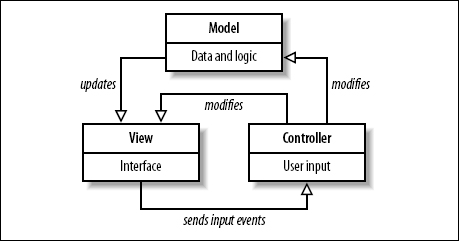
\includegraphics[width=0.9 \textwidth, keepaspectratio]{img/designPattern/mvc.jpg}
    \caption{Esempio di applicazione del design pattern MVC}
  \end{center}
\end{figure}
\begin{itemize}
\item \textbf{Scopo:} Disaccoppiare le tre seguenti componenti:
  \begin{itemize}
  \item Model: parte che si occupa direttamente di dati, logica e regole dell'applicazione;
  \item View: rappresentazione grafica sotto forma delle varie tipologie di output utilizzate per rappresentare i dati dell'applicazione;
  \item Controller: parte che accetta gli input e li converte in comandi per il model o la view;
  \end{itemize}
\item \textbf{Motivazione:} Molte applicazioni hanno la necessità di recuperare dati e di mostrarli in maniera opportuna agli utenti. Poiché si tratta di una comunicazione tra i dati dei dati e la interfaccia utente, bisogna trovare il metodo per far comunicare le due parti senza accorparle assieme, cosa che comporterebbe codice pesante e scarsa manutenibilità, in quanto in genere la parte grafica si evolve più in fretta della parte di model e, viceversa, bisogna rendere l'interfaccia che si offre all'utente quanto più separata possibile dall'implementazione effettiva della gestione dei dati. La soluzione che è stata trovata è costituita dal \gloss{design pattern} Model-View-Controller (MVC) che separa le tre componenti come già illustrato;
\item \textbf{Applicabilità:} Il pattern MVC è adatto ad essere utilizzato nei seguenti casi:
  \begin{itemize}
  \item se c'è la necessità che un insieme di oggetti debba essere considerato come un oggetto singolo;
  \item se c'è la necessità di disaccoppiare il model e la view, creando un sistema di notifiche tra le due componenti;
  \item Se c'è la necessità di avere più view per il medesimo model.
  \end{itemize}
\end{itemize}

\subsection{Design Pattern Creazionali}

\subsubsection{Singleton}

\begin{figure}[H]
  \begin{center}
    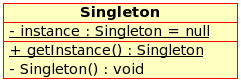
\includegraphics[width=0.3\textwidth, keepaspectratio]{img/designPattern/Singleton.png}
    \caption{Esempio di applicazione del design pattern singleton}
  \end{center}
\end{figure}

\begin{itemize}

\item \textbf{Scopo:} Assicurare che una classe abbia un'unica istanza ed avere
  un punto di accesso globale ad essa;

\item \textbf{Motivazione:} Per alcune classi è fondamentale assicurare che non
  abbiano più di un'istanza. Per questo motivo la classe tipicamente ha un
  costruttore privato e un metodo per poter accedere all'istanza della classe
  pubblico;

\item \textbf{Applicabilità:} Questo \gloss{design pattern} può essere
  applicato nei seguenti casi:
  \begin{itemize}
  \item Quando è essenziale che ci sia solo una istanza di una classe e tale
    istanza deve essere resa accessibile attraverso un unico punto di accesso;
  \item Quando l'unica istanza della classe deve essere estesa in maniera
    tale da non dover avere \gloss{client} con codici diversi.
  \end{itemize}

\end{itemize}

\subsubsection{Builder}

\begin{figure}[H]
  \begin{center}
    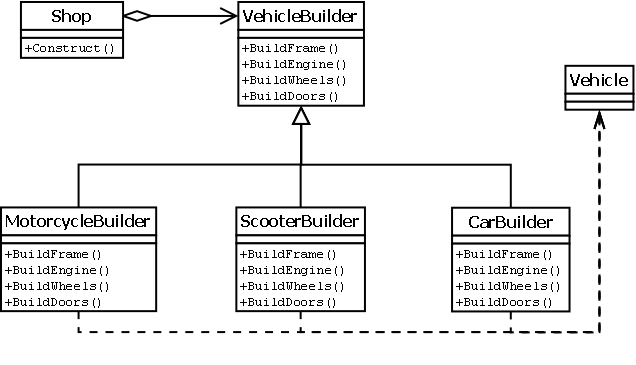
\includegraphics[width=0.3\textwidth, keepaspectratio]{img/designPattern/Builder.png}
    \caption{Esempio di applicazione del design pattern builder}
  \end{center}
\end{figure}

\begin{itemize}

\item \textbf{Scopo:} Permettere la crezione di oggetti complessi indipendentemente dalla
  sua rappresentazione;

\item \textbf{Motivazione:} Alcuni oggetti richiedono molti parametri di inizializzazione
  e possono avere molte rappresentazioni, questo porta spesso all'effetto \gloss{telescoping}
  dei costruttori di tale oggetto, e il \gloss{pattern} \gloss{abstract factory} risulta non essere
  abbastanza adeguato allo scopo;

\item \textbf{Applicabilità:} Questo \gloss{design pattern} può essere
  applicato nei seguenti casi:

  \begin{itemize}

  \item quando è necessaria la creazione di oggetti complessi con molte varianti
    di rappresentazione.

  \end{itemize}

\end{itemize}

\subsection{Design Pattern Strutturali}

\subsubsection{Decorator}

\begin{figure}[H]
  \begin{center}
    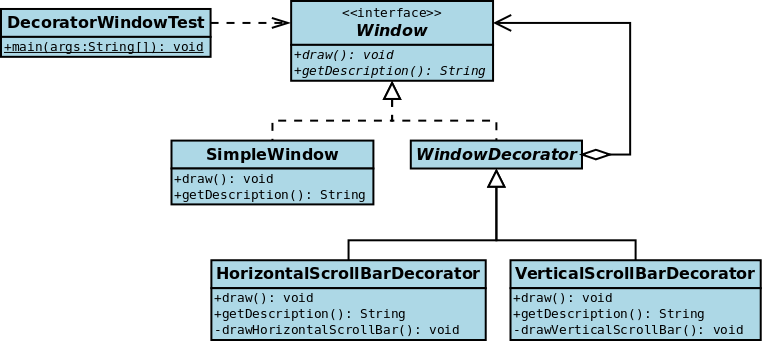
\includegraphics[width=0.7\textwidth, keepaspectratio]{img/designPattern/DecoratorPattern.png}
    \caption{Esempio di applicazione del design pattern decorator}
  \end{center}
\end{figure}

\begin{itemize}

\item \textbf{Scopo:} Aggiungere responsabilità e funzionalità dinamicamente ad oggetti già esistenti;


\item \textbf{Motivazione:} Permettere l'estendibilità di oggetti e affinare le funzionalità offerte
  modificandole o aggiungendone di nuove in modo trasparente.

\item \textbf{Applicabilità:} Questo \gloss{design pattern} può essere
  applicato nei seguenti casi:
  \begin{itemize}
  \item Quanto si presenta la necessita di riutilizzare un oggetto per le sue funzionalità, necessitando
    tuttavia di altre aggiuntive.
  \end{itemize}

\end{itemize}

\subsection{Design Pattern Comportamentali}

\subsubsection{Command}
\begin{figure}[H]
  \begin{center}
    \includegraphics[width=0.7\textwidth, keepaspectratio]{img/designPattern/CommandPattern.png}
    \caption{Esempio di applicazione del design pattern command}
  \end{center}
\end{figure}
\begin{itemize}
\item \textbf{Scopo:} Incapsulare una richiesta in un oggetto, cosicché il \gloss{client} sia indipendente dalle richieste, poiché le richieste hanno al loro interno tutti i dati necessari per essere risolte.
\item \textbf{Motivazione:} C'è la necessità di gestire richieste di cui non si conoscono i particolari poiché i Toolkit associano ai propri elementi, richieste da eseguire.
  Una classe astratta, Command, definisce l’interfaccia per eseguire la richiesta che è un semplice oggetto, per cui è possibile rendere variabile la reazione del \gloss{client} senza conoscere i dettagli dell'operazione stessa.
\item \textbf{Applicabilità:} Il Command pattern si presta bene alla parametrizzazione di oggetti sull’azione da eseguire (Callback function) soprattutto nello specificare, accodare ed eseguire richieste molteplici volte. Vi è inoltre il Supporto alle operazioni di "Undo" e "Redo". Vi è inoltre il supporto a transazione in quanto è possibile incapsulare un'azione in una operazione atomica.
\end{itemize}
\subsubsection{Observer}
\begin{figure}[H]
  \begin{center}
    \includegraphics[width=0.7\textwidth, keepaspectratio]{img/designPattern/Observer.png}
    \caption{Esempio di applicazione del design pattern observer}
  \end{center}
\end{figure}
\begin{itemize}
\item \textbf{Scopo:} Definisce una dipendenza “1..n” fra oggetti, riflettendo la modifica di un oggetto su quelli che ad esso dipendono.
\item \textbf{Motivazione:} Mantenere la consistenza fra oggetti, oltre che al modello e alle viste ad esso collegate.
  Observer pattern definisce come implementare la relazione di dipendenza: infatti il modello prevede due  attori principali che sono:
  \begin{itemize}
  \item Subject, che effettua le notifiche e contiene le interfacce per registrare e rimuovere gli observer;
  \item Observer, che si aggiorna in base alle notifiche che riceve dal subject.
  \end{itemize}
\item \textbf{Applicabilità:} È utile nei casi in cui si debba associare più “viste” differenti ad una astrazione. Il pattern comporta inoltre un aumento del grado di riuso dei singoli tipi;
  È indicato inoltre quando il cambiamento di un oggetto richiede il cambiamento di altri oggetti, oppure non si conosce quanti oggetti devono cambiare.
  È utile anche per notificare oggetti senza fare assunzioni su quali siano questi oggetti ed evita l’accoppiamento “forte”.
\end{itemize}

\newpage
\listoftables
\newpage
\listoffigures
\end{document}
